% Use only LaTeX2e, calling the article.cls class and 12-point type.
\documentclass[12pt]{article}

%=============== GEOMETRY AND PAGE LAYOUT ===============
\usepackage[textwidth=18.5cm, textheight=26cm]{geometry}
% The following parameters provide a reasonable page setup.
\topmargin 0.0cm
\oddsidemargin 0.2cm
\textwidth 16cm 
\textheight 21cm
\footskip 1.0cm

%=============== FONT AND LANGUAGE SUPPORT ===============
\usepackage{times}
\usepackage[english]{babel}
\usepackage[utf8]{inputenc}
\usepackage{textgreek}

%=============== MATH AND SCIENCE PACKAGES ===============
\usepackage{amsmath}
\usepackage{amssymb}
\usepackage{fourier}
\usepackage{siunitx}
\usepackage{mathtools}
\DeclareMathAlphabet\mathbfcal{OMS}{cmsy}{b}{n}
\DeclareMathAlphabet{\mathcal}{OMS}{cmsy}{m}{n}

%=============== GRAPHICS AND FIGURES ===============
\usepackage{graphicx}
\graphicspath{ {./fig/} }
\usepackage{subcaption}
\captionsetup[subfigure]{font={bf,small}, skip=1pt, margin=-0.1cm, singlelinecheck=false}
\usepackage[labelfont=bf]{caption}
\captionsetup{labelfont=bf, font=footnotesize}
\captionsetup[figure]{name={Fig.},labelsep=period}

%=============== TABLES ===============
\usepackage{tabularx,ragged2e,booktabs}
\usepackage{multirow}
\renewcommand{\arraystretch}{1.5} 

%=============== ACRONYMS ===============
\usepackage[nolist]{acronym}
\newacro{ai}[AI]{artificial intelligence}
\newacro{dai}[DAI]{disembodied artificial intelligence}
\newacro{eai}[EAI]{embodied artificial intelligence}
\newacro{gpu}[GPU]{graphics processing unit}
\newacro{cce}[CCE]{computation and communication expenditure}
\newacro{bee}[BEE]{basal energy expenditure}
\newacro{mie}[MIE]{motion and interaction expenditure}
\newacro{isl}[IsL]{isolated learning}
\newacro{il}[IL]{incremental learning}
\newacro{tl}[TL]{transfer learning}
\newacro{til}[TIL]{transfer with incremental learning}
\newacro{cl}[CL]{collective learning}
\newacro{dcl}[DCL]{distributed collective learning}

%=============== CUSTOM COMMANDS AND ENVIRONMENTS ===============
\usepackage{tcolorbox}
\usepackage{tikz}
\usetikzlibrary{backgrounds}
\usepackage{hyperref}
\usepackage{xcolor}
\usepackage{ulem} % For \xout

% Custom TikZ commands
\newcommand*\circled[1]{\tikz[baseline=(char.base)]{
    \node[shape=circle,draw,inner sep=2pt] (char) {#1};}}

% Custom highlighting and notes
\newcommand{\pending}[1]{\textcolor{blue}{$\bigstar$~\textbf{PENDING~#1}}}

% Custom math commands
\newcommand{\task}{\ensuremath{\tau}}
\newcommand{\sltwoi}{\ensuremath{t_l}} %single learning time without index
\newcommand{\slt}[1]{\ensuremath{t_{l,#1}}} %... with index
\newcommand{\tlt}{\ensuremath{T}} %total learning time
\newcommand{\comp}{\ensuremath{c}} %complexity (learning time from scratch)
\newcommand{\diste}[1]{\ensuremath{\mathrm{d}(\task_{#1},\{ \})}}
\newcommand{\dist}[2]{\ensuremath{\mathrm{d}(\task_{#1},\{\task_1, \task_2, \dots, \task_{#2}\})}}
\newcommand{\En}{\ensuremath{E}}
\newcommand{\opt}{\ensuremath{\mathrm{opt}}}
\newcommand{\tot}{\ensuremath{\mathrm{tot}}}
\newcommand{\Opt}{\ensuremath{\mathrm{Opt}}}
\newcommand{\densMan}{\ensuremath{\rho_{\mathrm{man}}}} %manufacturing energy density
\newcommand{\Tau}{\ensuremath{\mathcal{T}}}

% Custom environments
\newenvironment{sciabstract}{%
\begin{quote} \bf}
{\end{quote}}

\makeatletter
\tikzset{%
    fancy quotes/.style={
        text width=\fq@width pt,
        align=justify,
        inner sep=1em,
        anchor=north west,
        minimum width=\linewidth,
    },
    fancy quotes width/.initial={.8\linewidth},
    fancy quotes marks/.style={
        scale=8,
        text=white,
        inner sep=0pt,
    },
    fancy quotes opening/.style={
        fancy quotes marks,
    },
    fancy quotes closing/.style={
        fancy quotes marks,
    },
    fancy quotes background/.style={
        show background rectangle,
        inner frame xsep=0pt,
        background rectangle/.style={
            fill=gray!25,
            rounded corners,
        },
    }
}

\newenvironment{fancyquotes}[1][]{%
    \noindent
    \tikzpicture[fancy quotes background]
    \node[fancy quotes opening,anchor=north west] (fq@ul) at (0,0) {``};
    \tikz@scan@one@point\pgfutil@firstofone(fq@ul.east)
    \pgfmathsetmacro{\fq@width}{\linewidth - 2*\pgf@x}
    \node[fancy quotes,#1] (fq@txt) at (fq@ul.north west) \bgroup
}
{\egroup;
    \node[overlay,fancy quotes closing,anchor=east] at (fq@txt.south east) {''};
\endtikzpicture}
\makeatother

% Cross-referencing supplementary material
\usepackage{xr}
\externaldocument{supplementary_materials}

% Line numbering for review
\usepackage{lineno}
\linenumbers

\newtheorem{assumption}{Assumption}
\newtheorem{definition}{Definition}
\newtheorem{challenge}{\textbf{CHALLENGE}}

%%%%%%%%%%%%%%%%% END OF PREAMBLE %%%%%%%%%%%%%%%%

\begin{document} 
\baselineskip24pt % Double-space the manuscript.

\title{\textbf{REVISED Tackling AI Sustainability: Collective Learning for Energy Efficiency}}

\author
{\textbf{Fernando D\'iaz Ledezma$ {}^{1,\ast}$ and Sami Haddadin${}^{2}$}
    \\
    \normalsize{\textbf{Affiliations:} ${}^{1}$TUM - Technical University of Munich}\\
    \normalsize{${}^{2}$MBZUAI - Mohamed bin Zayed University of Artificial Intelligence}\\
    \\
    \normalsize{$^\ast$To whom correspondence should be addressed; E-mail: fernando.diaz@tum.de}
}

\date{}

\maketitle 

\begin{sciabstract}
The current learning paradigms in \ac{dai} are characterized by substantial energy consumption, primarily due to intensive computational processes and limited utilization of acquired knowledge. As \ac{ai} converges with robotics to form \ac{eai} systems, their energy demands are poised to escalate further because data acquisition and learning necessitate continuous interaction with the physical environment. This study delves into the core energy requirements of \ac{eai} systems and explores the energy-related challenges linked to maintaining existing learning paradigms. Consequently, we advocate for collective learning, a paradigm shift that promotes efficient learning in \ac{eai} agents by actively sharing, aggregating, and leveraging past and current knowledge across systems. This approach is pivotal for reducing energy consumption and expediting the acquisition of new skills.
\end{sciabstract}

\section*{Main Text}

AI-powered technology, especially machine learning, is increasingly integrated into daily life. We anticipate a future with smart factories, AI-enhanced healthcare services, and automated homes. Modern robots, equipped with advanced computing and communication capabilities, will become ubiquitous in industry, logistics, service, and healthcare. These robots will leverage AI to acquire new skills and share knowledge across systems, integrating synergistically with various environments and collaborating with humans on diverse tasks. However, this growing ubiquity of AI and robotics also presents significant challenges, particularly concerning their energy demands.

The rapid advancements driven by AI applications come at a substantial energy cost. Cutting-edge machine learning algorithms demand immense computational power to process, analyze, and learn from vast datasets, often requiring numerous iterations to converge \cite{Strubell2019EnergyPolicyConsiderations}. Researchers and corporations rely heavily on existing infrastructure or cloud computing services in data centers for these energy-intensive workloads during both learning and deployment phases. This has led to a clear spike in energy consumption in data centers and associated hardware like GPUs. Training AI models in data centers is estimated to consume about three times more energy than traditional cloud tasks, significantly straining resources \cite{Thomas2023cloudusesmassive}. Consider the latest breakthroughs in generative AI, including large language models (LLMs) and text-to-image models. These models, with billions of parameters, require thousands of deep learning GPU units and millions of GPU hours for training \cite{Vanian2023ChatGPTgenerativeAI, Corbyn2023Nvidiachipmaker}. As more AI applications are developed, the demand for AI infrastructure surges, leading to a substantial increase in GPU-based AI server sales. This escalation directly translates to a parallel rise in data center energy consumption. Globally, data center energy consumption soared from 200 TWh in 2015 to an estimated 220-320 TWh in 2021, according to the International Energy Agency\footnote{Data from the International Energy Agency, available at \url{https://www.iea.org/reports/data-centres-and-data-transmission-networks}}. This concerning trend is illustrated in Fig.~\ref{fig:energy_consumption_trends_ai_and_robotics} (\textsc{Left} panel).

The second challenge, the escalating energy demand of a robotic revolution, is amplified by the rise of Industry 4.0, the implementation of smart factories, and the expanding use of robots in service applications. This rapid proliferation has even been dubbed the "Cambrian explosion" of robotics \cite{Pratt2015Iscambrianexplosion}. Despite advancements in robot technology that have improved energy efficiency, the focus remains predominantly on individual systems, often overlooking the aggregate impact of all active units. Over the past decade, the installed base of industrial robots has undergone a remarkable transformation. According to the International Federation of Robotics (IFR), this base surged from 1.2 million units in 2012 to approximately 4.2 million units in 2023—an astonishing 350\% increase with an average annual growth rate close to 12\% \cite{IFR2024WorldRobotics2024}. Extrapolating this trend suggests that within the coming years, six million robots will be operational in factories worldwide\footnote{These projections closely align with the slightly more cautious estimates presented by \textit{The Boston Consulting Group} in \cite{Sirkin2015HowRobotsWill}.}. Using this estimated installed base and assuming round-the-clock operation, we can approximate the forthcoming energy demand attributable to industrial robots, termed the World Robot Energy Consumption (WREC), as shown in Fig.~\ref{fig:energy_consumption_trends_ai_and_robotics} (\textsc{Middle} panel). To contextualize the significance of WREC, in 2025, it is projected to constitute 7.2\% of Germany's installed electricity generation capacity \cite{FraunhoferISENetinstalledelectricity}. A detailed description of these estimates is provided in Sec.~\ref{sec:app_robot_ener_consumption}. The far-reaching influence of collaborative and service robots mirrors the significance observed among their industrial counterparts. Collaborative robots (cobots), for instance, have undergone a paradigm shift, rising from a mere 6\% of the market in 2017 to constituting around one-quarter of annual installations \cite{tobe2015}, as illustrated in Fig.~\ref{fig:industrial_cobot_share}. Drawing from analogous assumptions applied to industrial robots, Fig.~\ref{fig:energy_consumption_trends_ai_and_robotics} (\textsc{Right} panel) depicts the projected growth trajectory of cobots and their associated energy consumption. Concurrently, the domain of service robots is experiencing an analogous surge. For instance, estimates project that the service robotics market will reach 56 billion euros in 2025 \cite{statista_service_robots}. These robots are utilized across various fields, including logistics, defense, public relations, and medical applications, aligning with the escalating trends observed among industrial and collaborative robots. The third challenge, often overlooked, is the energetic expenditure associated with manufacturing the hardware required for AI and robotics. This energy demand encompasses two primary facets. First, it involves the energy outlay for procuring materials for robot manufacturing and associated computational hardware (e.g., processors, GPUs, and AI servers). Second, it pertains to the energy consumption intrinsic to the manufacturing process itself. Given the direct correlation between energy demand and the number of AI-powered robots produced, an exponential rise in the latter directly corresponds to escalated energy consumption for their production. The assessment and formulation of strategies to address this aspect are crucial. While an immediate solution may not be evident, and substantial energy savings in raw material procurement may be impractical, significant potential lies in the recycling of electronic components of computer and robot hardware as a means of conserving energy\footnote{An example of such an endeavor is the international competition \textit{Robothon\textsuperscript{\textregistered} - The Grand Challenge}, see~\url{https://automatica-munich.com/en/munich-i/robothon/}.}.

\begin{figure*}[t!]
	\centering
	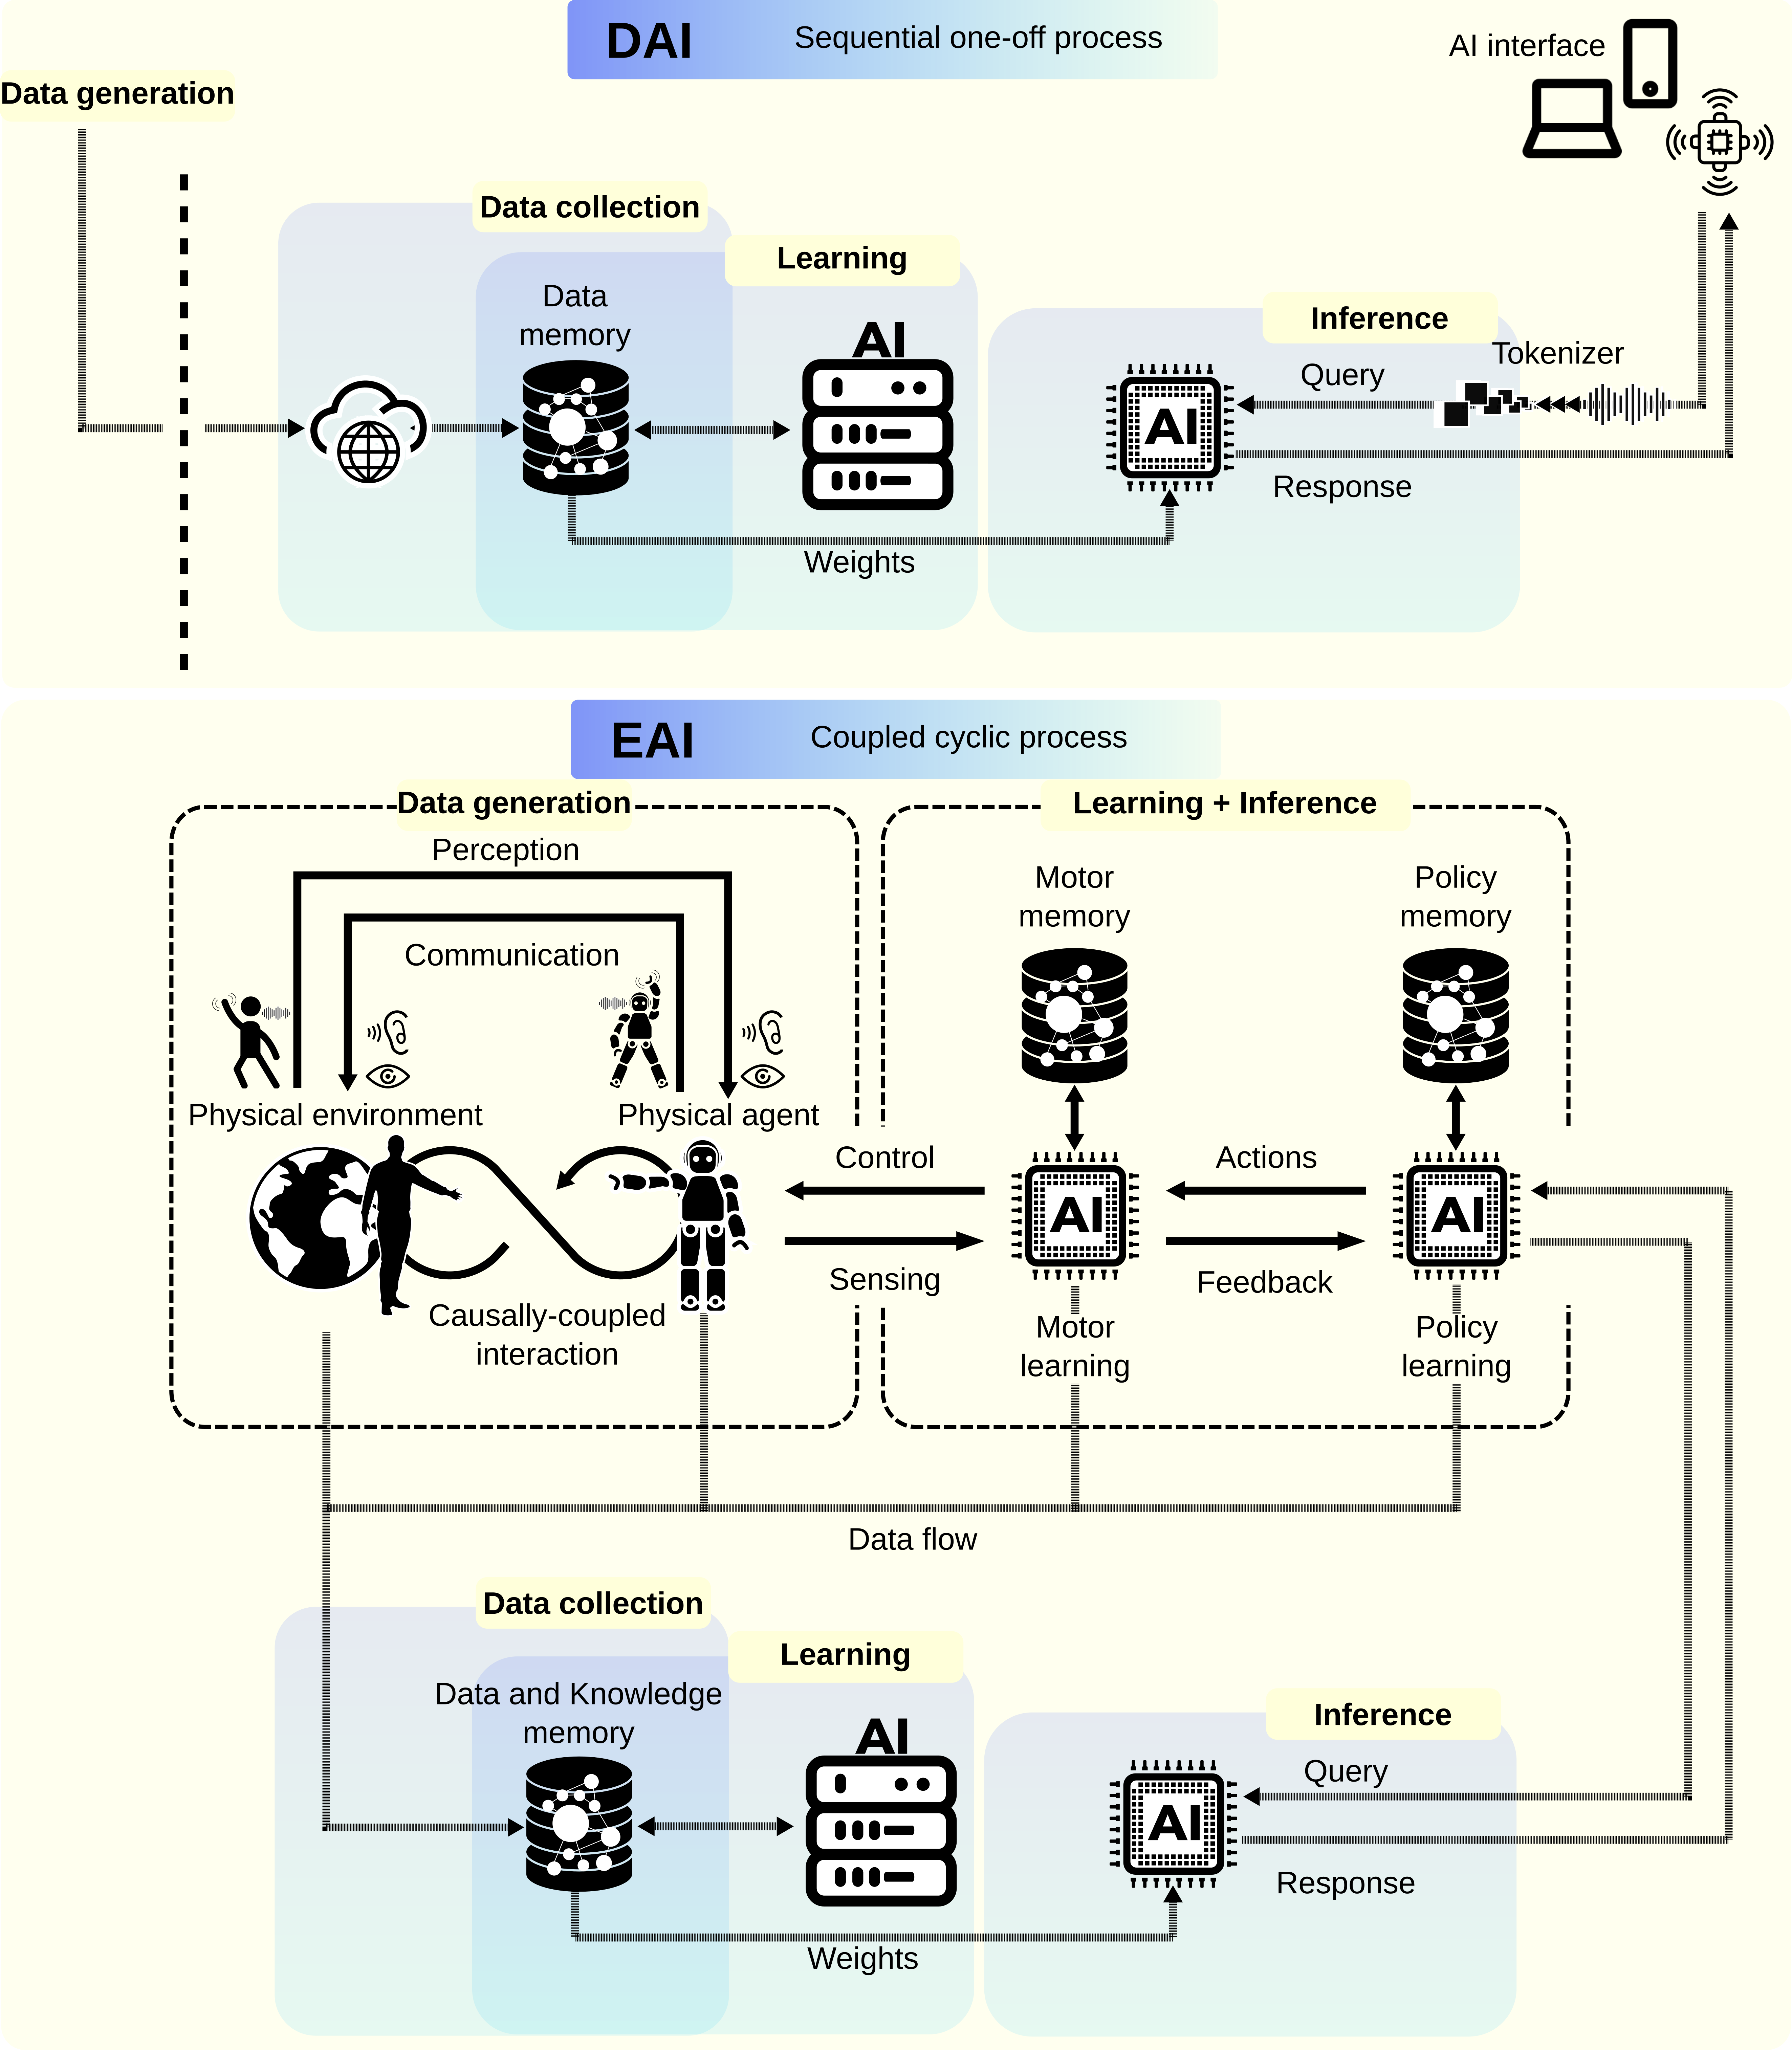
\includegraphics[width=0.95\textwidth]{eai_and_dai_concept_figure.png}
	\caption[] {\label{fig:eai_and_dai_concept_figure} \textbf{Disembodied and embodied \ac{ai}.} \textsc{TOP}: In \ac{dai} learning is a sequential one-off process from which data generation is detached. \textsc{Bottom}: Causally-coupled cyclic interaction of \ac{eai} agents with the environment generates data for learning.}
\end{figure*}

\paragraph*{Energy Expenditure in Disembodied and Embodied AI.}
To effectively address the energy demands of AI and robotics, we differentiate between classical \ac{dai} and \ac{eai}, as illustrated in Fig.~\ref{fig:eai_and_dai_concept_figure}. We define DAI as methods and algorithms that tackle purely computational problems, detached from embodied systems and lacking interaction with the physical world (see Fig.~\ref{fig:eai_and_dai_concept_figure}, \textsc{Top} panel). In DAI, data collection occurs passively through various edge devices, with a prototypical DAI agent not directly involved in generating or collecting training data. The energetic demands of DAI applications primarily stem from learning (training models) and deployment (running inference and prediction) \cite{Vries2023growingenergyfootprint}. For DAI applications targeting diverse tasks or systems, successful knowledge transfer relies on the adequacy of the learning paradigm and both model and training data carrying enough information about the problem. However, in the absence of any of these factors, retraining, sometimes from scratch, becomes necessary, leading to highly energy-inefficient learning processes. Even if learning occurs only once, the ongoing deployment of the model can demand significant energy due to constant computationally intensive execution \cite{Vries2023growingenergyfootprint}. Thus, depending on the application, the energetic cost of learning and deployment in DAI can outweigh the benefits \cite{Strubell2019EnergyPolicyConsiderations}. This also applies to recent breakthroughs, such as transformer models for Natural Language Processing, whose results are accompanied by energetic challenges \cite{Cao2020TowardsAccurateReliable}.

The evolution toward EAI, the integration of AI and robotics \cite{Pfeifer2004Embodiedartificialintelligence}, expands the energy usage spectrum. Unlike virtual environments, the real world cannot be faithfully replicated, despite considerable advances in sim-to-real applications \cite{Chebotar2019Closingsimreal}. Learning and deployment in EAI demand constant, energy-expending interaction with the physical environment for active data generation, as depicted in the \textsc{Bottom} panel of Fig.~\ref{fig:eai_and_dai_concept_figure}, facilitated by physical agents like robots, vehicles, and drones. Mastering skills in the physical realm requires continuous and repeated execution, consuming energy for motion and interaction in each instance. Take autonomous driving, for example, where vehicles function as rudimentary EAI agents in structured human-made environments. Besides energy for autonomous movement, vehicles expend additional energy on motion to collect data necessary for retraining and improving the policy model. Another example is the usage of household robots to automate a high percentage of domestic chores \cite{Lehdonvirta2022futuresunpaidwork}. Such robots will undergo constant retraining due to the subtle and changing dynamics of household environments.

\begin{figure*}[t!]
	\centering
	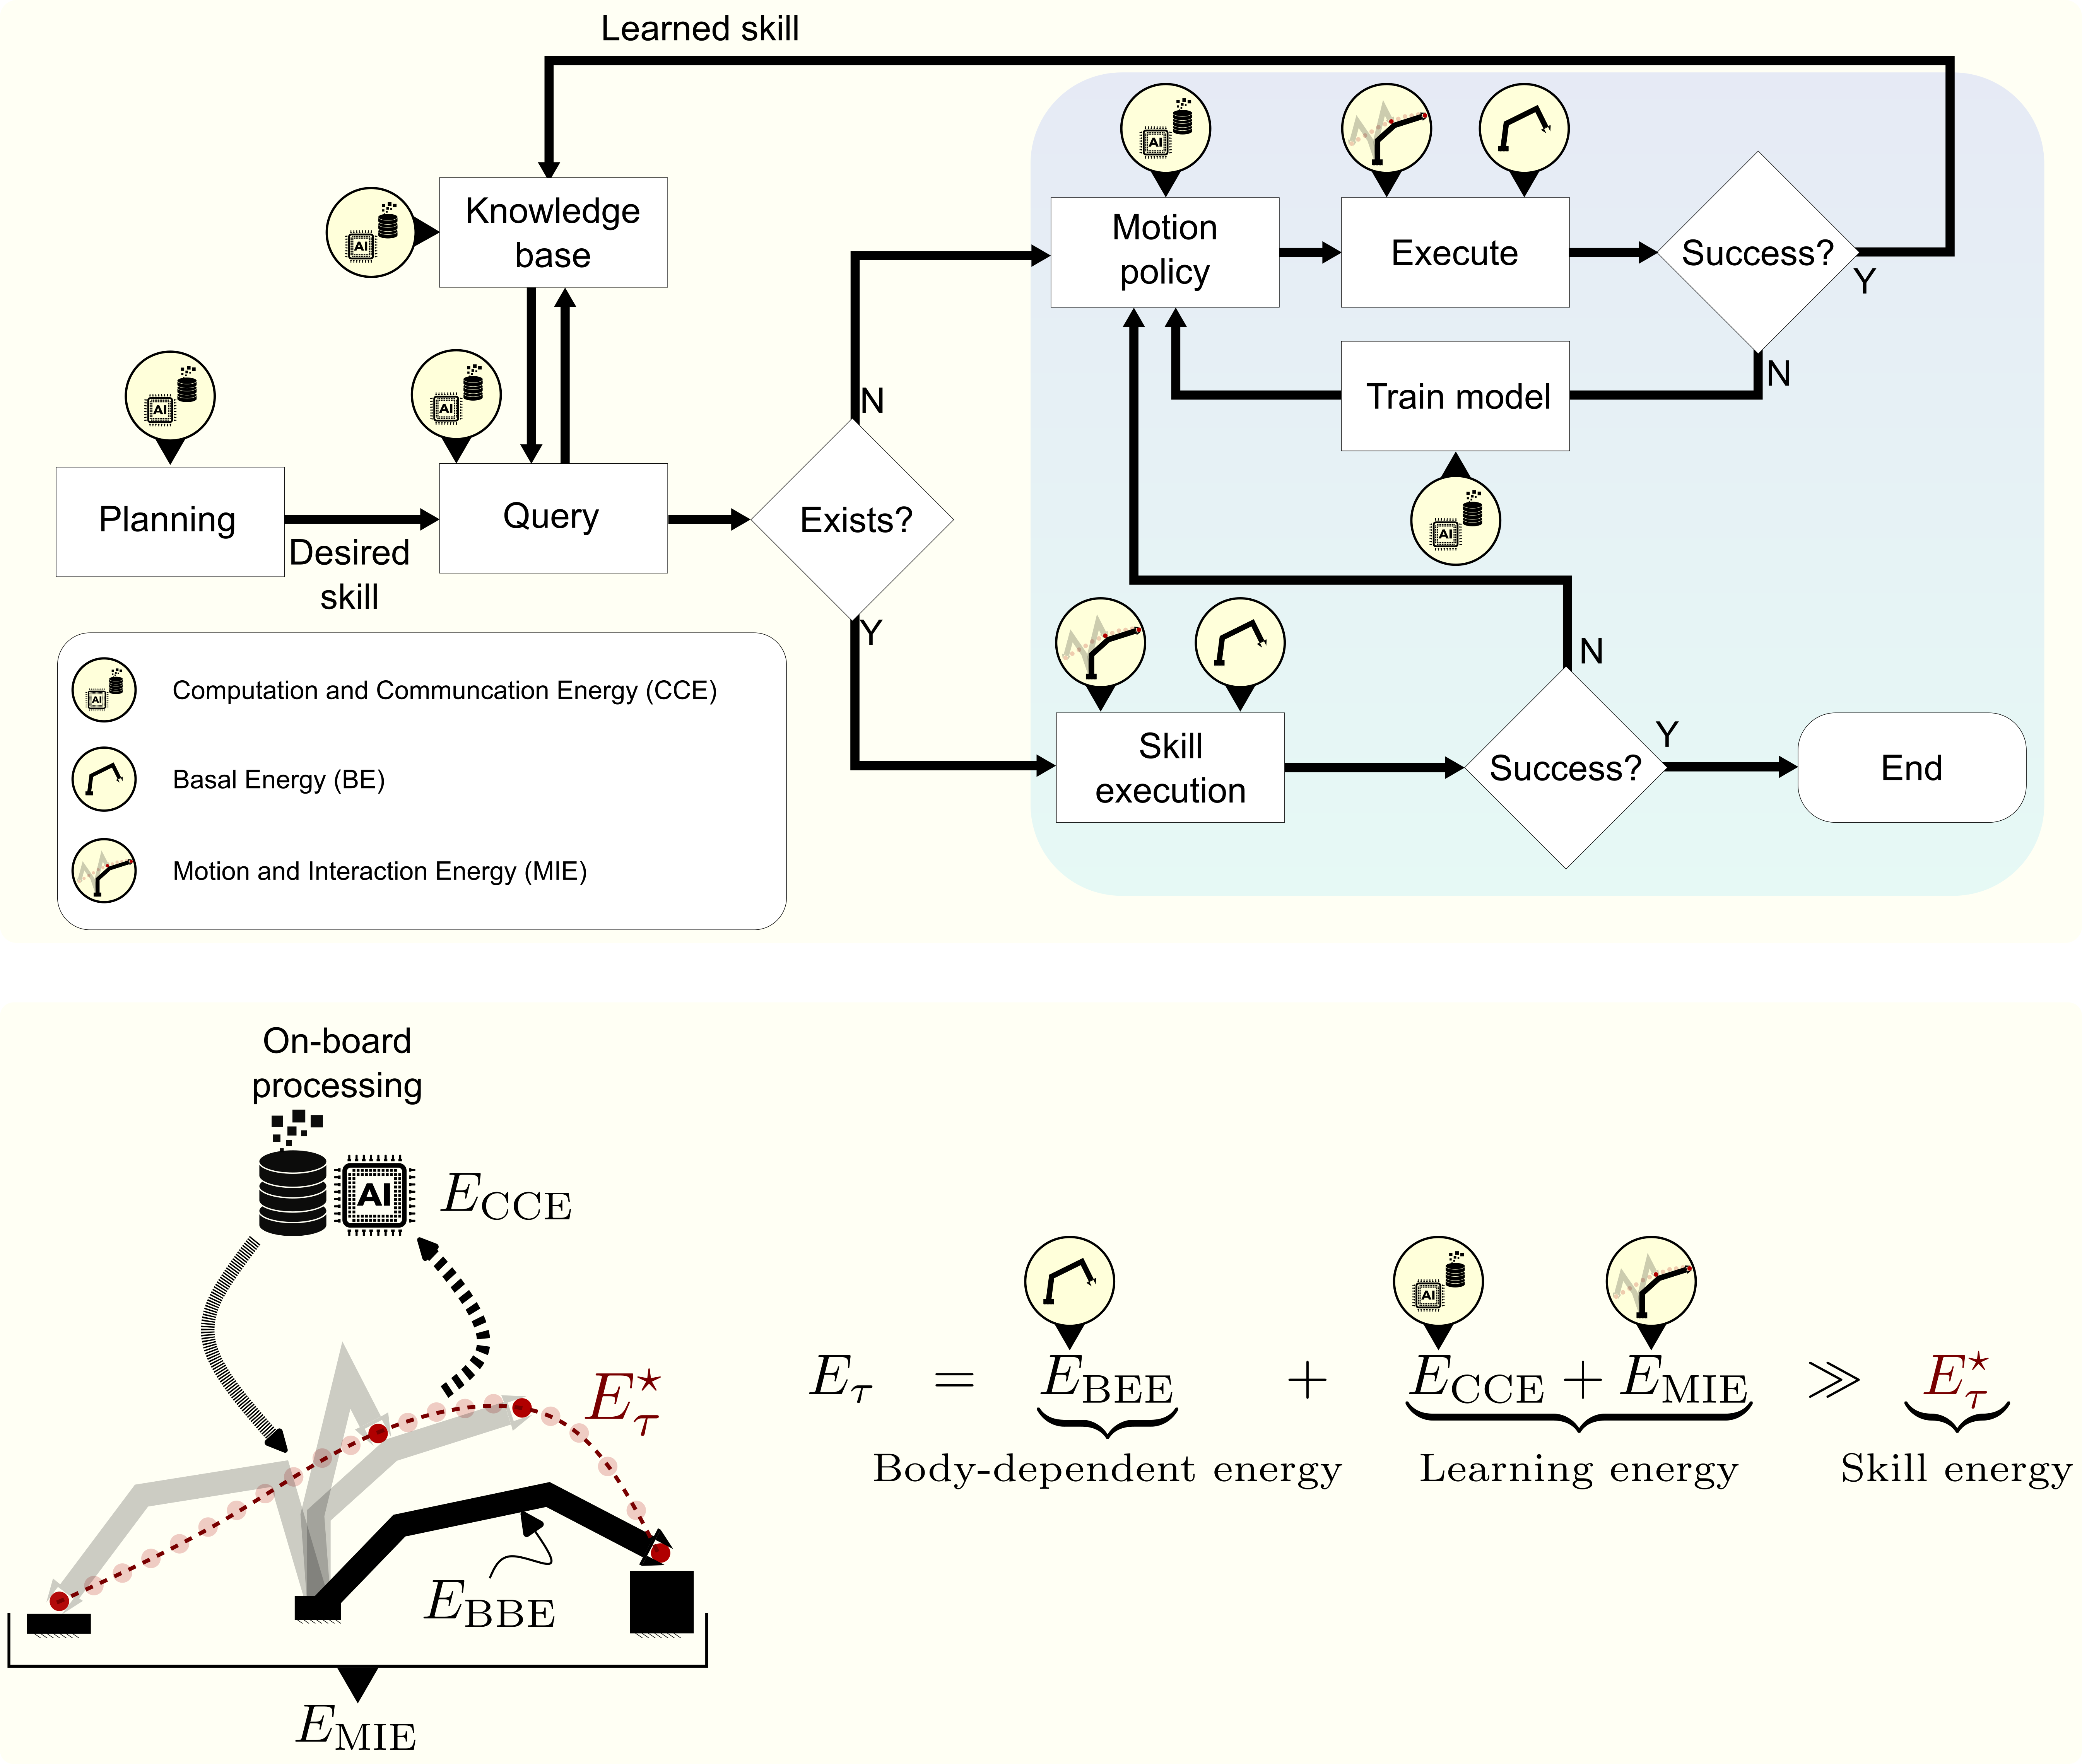
\includegraphics[width=0.95\textwidth]{eai_energy_categories.png}
	\caption[] {\label{fig:embodied_ai_pipeline} \textbf{Energy expenditures of an \ac{eai} agent.} {\textsc{Top}: Standard skill execution pipeline of a prototypical \ac{eai} agent. \textsc{Bottom}: Three fundamental energy expenditure categories are identified during the planning, learning, and execution of a skill by an \ac{eai} agent.}}
\end{figure*}

Unlike the standard energy classification for learning and deployment in \ac{dai}, analyzing energetic requirements in \ac{eai} demands a different perspective. A closer look at the standard skill execution pipeline of a prototypical \ac{eai} agent (Fig.~\ref{fig:embodied_ai_pipeline}) allows for the identification of essential energetic expenditure categories:
\begin{enumerate}
	\item \Acl{cce}: Coincident with DAI, this refers to the energy used by computational and communication processes required for planning, querying, exploration, and training routines.
	\item \Acl{bee}: This body-related energy is associated with the execution of basic functions of the EAI agent. Examples include operating energy, gravity compensation, and proprioceptive intelligence algorithms in robots, hovering in drones, and running on-board system standby in autonomous vehicles.
	\item \Acl{mie}: This defines the energy expended on physical interactions, specifically executing a particular skill. For instance, moving an object from an initial to a target location within a given time following a particular trajectory.
\end{enumerate}

An important fact in \ac{eai} is the existence of a lower bound on the energy required to carry out a skill that is independent of the agent. Consider a generic skill $\tau$---such as a pick-and-place operation---and suppose the optimal trajectory $p^\star$ for moving an object from its origin to its destination is known. The intrinsic properties of the object and the optimal trajectory $p^\star$ uniquely define the minimum energy requirement $E^\star_{\tau}$ needed to perform skill $\tau$. The implication is that the total energy expended by any agent in the process of mastering or executing a skill is higher than $E^\star_{\tau}$ as a result of the required computational ($E_\text{CCE}$), body-related ($E_\text{BEE}$), and physical interaction ($E_\text{MIE}$) energy expenditures; i.e.,
\begin{equation}\label{eq:skill_energy_in_eai_revised}
	E_{\tau} =  \underbrace{E_\text{BEE}}_{\text{Body-dependent energy}} + \underbrace{E_\text{CCE} + E_\text{MIE}}_{\text{Learning energy}} \gg \underbrace{E^\star_{\tau}}_{\text{Skill energy}}.
\end{equation}
It is worth mentioning that if Eq.~\eqref{eq:skill_energy_in_eai_revised} were used to describe the energy consumption of a task in \ac{dai}, $E_\text{BEE}$ could be associated with the edge devices, and $E_\text{CCE}$ would represent the primary source of energy consumption. Additionally, the expenditures $E^\star_{\tau}$ and $E_\text{MIE}$ do not exist in \ac{dai} since physical interaction is absent.

\paragraph*{Related Works}
The growing trends depicted in Fig.~\ref{fig:energy_consumption_trends_ai_and_robotics} suggest that the energy expenditures for computation and communication, basal functions, and motion and interaction will likely follow a similar pattern. The implication is straightforward: as the number of \ac{ai} applications and robotic systems increases, so does their associated energy demand. Consequently, the energy requirements of \ac{dai} and \ac{eai} have recently received significant attention within the \ac{ai} and robotics research communities. The escalating energy consumption of \ac{ai}, particularly machine learning, has raised concerns about its adverse environmental impact. Most research in this area focuses on the computational and infrastructural requirements for training and running modern learning algorithms---such analyses directly correlate with computational and communication energy expenditure. Recent works have delved into the efficiency of computation-intensive deep learning algorithms \cite{Schwartz2019GreenAI,Vinuesa2020roleartificialintelligence,Strubell2019EnergyPolicyConsiderations,Luccioni2023EstimatingCarbonFootprint}. In parallel, various metrics have been established to gauge the energy consumption of machine learning algorithms. These include assessing energy efficiency during development phases \cite{Zhou2020HULKEnergyEfficiency}, analyzing accuracy, model size, time, and CPU/GPU energy consumption for training and inference phases \cite{Dalgren2019GreenMLmethodology}, as well as encompassing other system-level performance indicators like real-time metrics, instruction-level analysis, and hardware-level power estimation \cite{GarciaMartin2019Estimationenergyconsumption}. Recent works on large language models have discussed various aspects such as hardware efficiency, model architectures, and algorithms in relation to energy consumption \cite{Vries2023growingenergyfootprint} and provide comparisons including their power consumption and CO$_2$ emissions \cite{SIHCAI2023ArtificialIntelligenceIndex}. Despite growing awareness of \ac{ai}'s energy consumption, tangible actions to address underlying issues and propose remedies remain scarce and predominantly focus on \ac{dai} applications. Yet, it is crucial to recognize the challenges posed by \ac{eai} systems. Unlike state-of-the-art machine learning models (e.g., transformer models) that are mostly trained once on a large amount of data, \ac{eai} agents have a constant need for energy-consuming retraining and evaluation processes. From the \ac{eai} perspective, ongoing efforts to minimize \ac{bee} and improve \ac{mie} advocate strategies such as elastic actuation and optimized hardware selection and storage, energy sharing, and motion planning \cite{CUT2015Smoothrobotmovements, Mohammed2014MinimizingEnergyConsumption, Chemnitz2011Analyzingenergyconsumption,Vasarhelyi2023OverviewEnergiesProblems,Sekala2024SelectedIssuesMethods}. As for \ac{cce}, it is essential to design better hardware for more efficient parallel computing and to decentralize the computation, leveraging the local processing capabilities of edge devices and robots. These capabilities have been highlighted in concepts such as the Internet of Robotic Things \cite{Vermesan2020InternetRoboticThings,Sekala2024SelectedIssuesMethods}. Perhaps even more relevant is to define sample-efficient algorithms with optimized models that account for the recurrent learning, inference, and prediction processes in \ac{eai} agents. We believe that achieving greater energy efficiency in \ac{ai} requires a broader perspective than just enhancing hardware and optimizing the individual agents' learning strategies. The actual key to a significant breakthrough lies in tapping into the vast reservoir of knowledge accumulated by \ac{eai} systems.

\paragraph*{\Acl{cl} for \ac{eai}}
The rapid proliferation of robotic agents and advances in \ac{ai} present a pressing challenge: the rising energy demands of contemporary learning paradigms. These paradigms---primarily designed for disembodied systems---often overlook the potential of systematic knowledge sharing across agents, resulting in significant inefficiencies in large-scale robotic deployments. As robots increasingly rely on interaction-intensive learning and adaptation, the absence of coordinated knowledge exchange exacerbates both computational and mechanical energy consumption. This raises a fundamental question: \emph{How can robotic systems learn effectively while minimizing energy usage?} We address this by positing the paradigm of \acl{cl} \cite{Haddadin2014SystemzumErstellen,Haddadin2015Systemgeneratingsets}, a learning strategy tailored to improve energy efficiency in \ac{eai}. \Ac{cl} capitalizes on inter-agent connectivity and structured knowledge sharing, enabling robots to acquire and share skills more efficiently, thereby reducing redundant computation and unnecessary physical interaction. This work investigates the dynamics of optimal knowledge sharing in robotic collectives, laying the groundwork for more energy-aware and sustainable \ac{ai}-driven robotics. The \ac{cl} concept encapsulates the dynamic, progressive creation and augmentation of knowledge through interactive processes. In this framework, knowledge from individuals is actively exchanged, spread, and enhanced, fostering a deeper, more comprehensive understanding that evolves over time \cite{Garavan2012CollectiveLearning}. Fundamental aspects of \ac{cl} particularly relevant to \ac{eai} agents include the aggregation of skills, knowledge, and behaviors. This concept is loosely related to collective intelligence and swarm intelligence \cite{Beni2004SwarmIntelligenceSwarm,Blum2015SwarmIntelligenceOptimization,Dorigo2021SwarmRoboticsPast}, collaborative, federated, and distributed learning \cite{Technologie2023FLAIROPFederatedLearning,Anjos2023SurveyCollaborativeLearning,Xianjia2021Federatedlearningrobotic,Sartoretti2019DistributedLearningDecentralized,Sartoretti2018DistributedLearningDecentralized,Wang2022DistributedReinforcementLearning}, networked robotics \cite{Kumar2008NetworkedRobots}, and fleet learning \cite{Wang2023RobotFleetLearning}. Arguably, the many contributions in these areas have addressed various underlying principles of collective systems \cite{Kernbach2013HandbookCollectiveRobotics}. Nevertheless, these approaches do not target the hypothesized exponential learning resulting from \ac{cl} \cite{Haddadin2019Breakingwallcollective}. Furthermore, the specific algorithms required to effectively realize \ac{cl}---in particular, for knowledge acquisition, transfer, distribution, and integration---are still nonexistent or currently under development \cite{Haddadin2022collectivelearningtheory}. Despite this, the expectation is that an appropriate learning algorithm capable of leveraging the body of knowledge accumulated by a multi-agent system (a \emph{collective}) can shape the knowledge acquisition dynamics of the entire system, positively impacting the learning time and energy efficiency of new skills.

\section*{Results}\label{sec:results}

\begin{figure*}[t!]
	\centering
	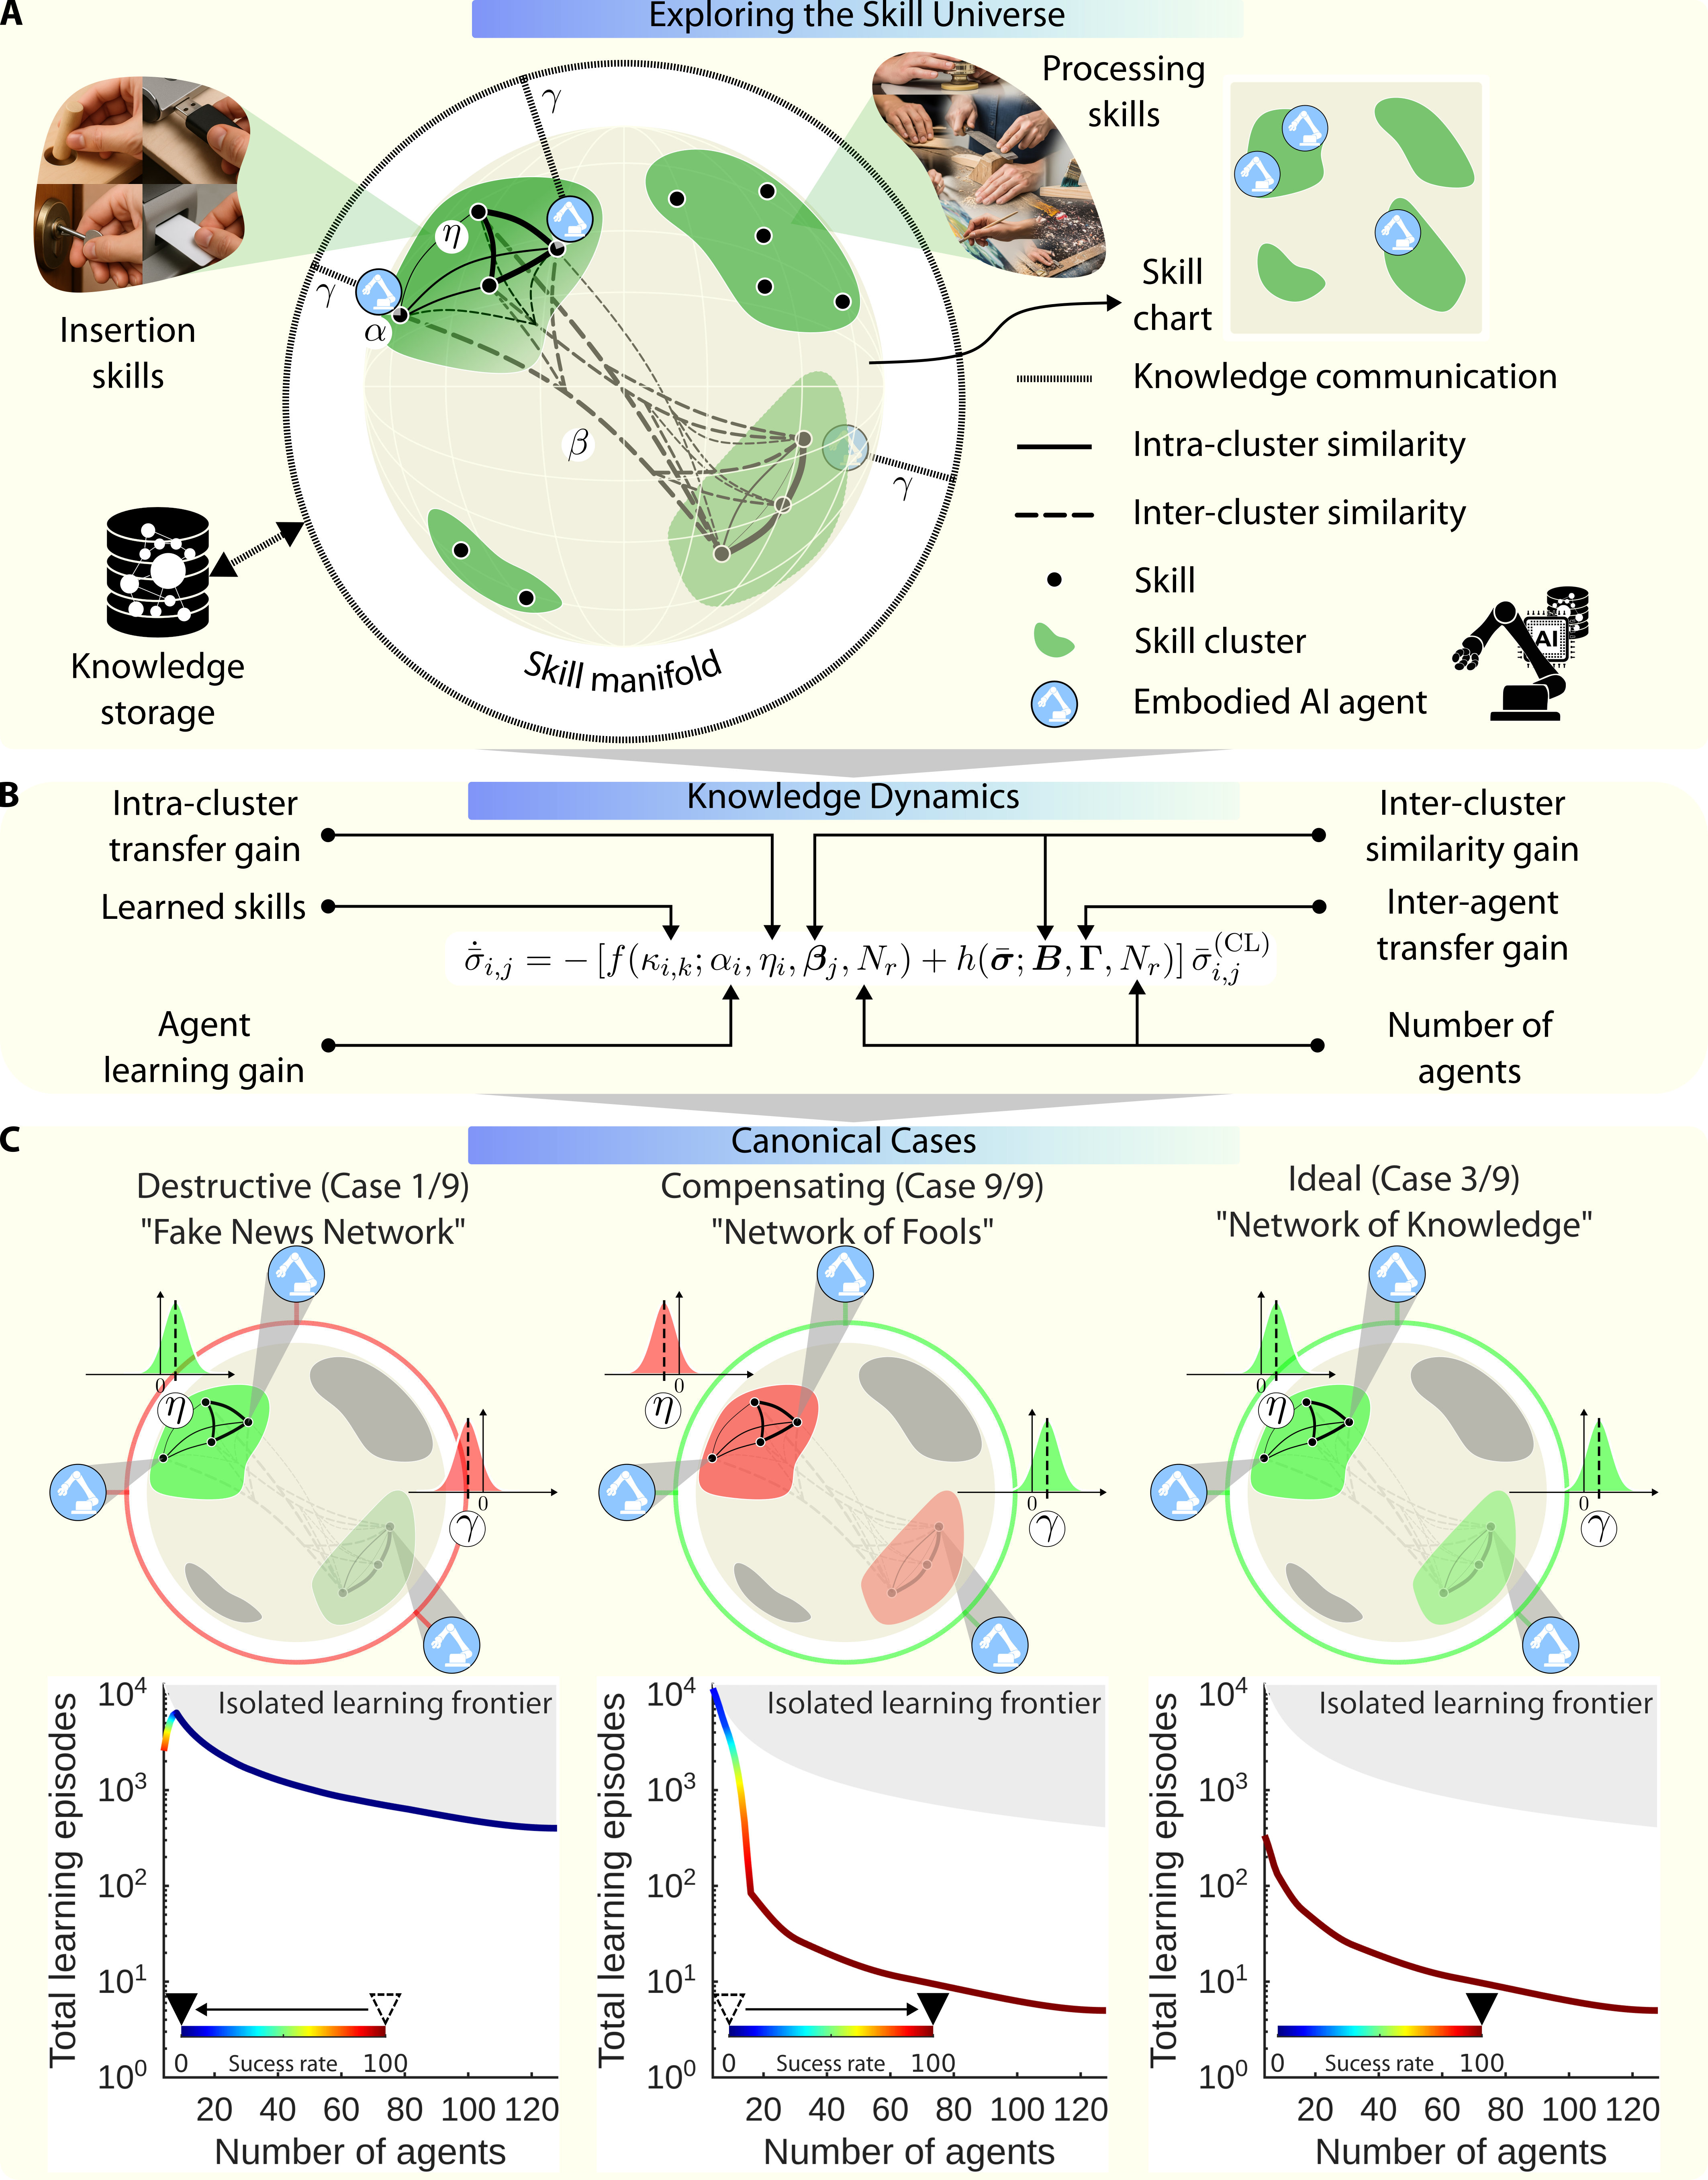
\includegraphics[width=14cm]{collective_learning_and_skill_manifold_conceptualization.png}
	\caption[] {\label{fig:collective_learning_and_skill_manifold_conceptualization_revised} \textbf{Collective learning dynamics over a structured skill manifold.} \textsc{Top}: \ac{eai} agents learn and share knowledge across a structured \textit{skill manifold}, where skills form clusters with intra- and inter-cluster similarity. \textsc{Middle}: The skill remaining knowledge dynamics $\dot{\bar{\sigma}}^{(\mathrm{CL})}_j$. \textsc{Bottom}: Three representative \ac{cl} regimes: \textit{Destructive} (learning inhibited by poor communication), \textit{Compensating} (weak agents supported by strong network), and \textit{Ideal} (synergistic learning across agents and network).}
\end{figure*}

\paragraph*{\Acl{cl} of skills}
Fig.~\ref{fig:collective_learning_and_skill_manifold_conceptualization_revised} presents a conceptual and quantitative illustration of the structure of a robot collective learning a distribution of skills and the associated knowledge dynamics governing \ac{cl} in \ac{eai} systems. The \textsc{top} panel visualizes the notion of a \textit{skill manifold}, a continuous and structured latent space that organizes the knowledge of a population of skills. Individual skills are grouped into \textit{skill clusters} based on their shared similarity. The \ac{eai} agents navigate this manifold by learning skills and exchanging knowledge with peers. The strength of agent-level skill knowledge integration is quantified by $\eta$, while $\gamma$ captures the quality of inter-agent knowledge exchange. The \textsc{middle} panel formalizes the dynamics of the remaining knowledge about a skill, $\dot{\bar{\sigma}}^{(\mathrm{CL})}_j$. The governing equation, Eq.\eqref{eq:collective_knowledge_dynamics_revised}, depends on four main terms: \emph{agent learning gain} ($\alpha$), \emph{intra-cluster knowledge sharing gain} ($\eta$), \emph{inter-cluster similarity gain} ($\beta$), and \emph{inter-agent transfer gain} ($\gamma$). These components determine whether knowledge about a skill decays (successful learning) or grows (corruption or forgetting).

Let a skill learning scenario be $\phi = (N_\mathcal{S}, N_\mathcal{K}, N_\mathrm{r}, \bm{\rho})$, where $N_\mathcal{S}$ is the number of skills, $N_\mathcal{K}$ the number of clusters, $N_\mathrm{r}$ the number of agents, and $\bm{\rho}$ defines the knowledge exchange efficiency. We discuss a scenario where a collective learns $N_\mathcal{S}=512$ skills in $N_\mathcal{K}=4$ clusters. A skill is learned when the remaining knowledge $\bar{\sigma}$ is below $\epsilon = 0.01$. The fundamental complexity is $c_0 = 100$ episodes, and the energy cost per episode is $e_0$. The \textsc{bottom} panel of Fig.~\ref{fig:collective_learning_and_skill_manifold_conceptualization_revised} illustrates three operating regimes based on the mean values $(\bar{\eta}, \bar{\gamma})$. In the \textbf{destructive regime} ($\bar{\eta} > 0, \bar{\gamma} < 0$), competent agents are undermined by noisy collective interactions. In the \textbf{compensating regime} ($\bar{\eta} < 0, \bar{\gamma} > 0$), a well-functioning collective counteracts poor individual learners. In the \textbf{ideal regime} ($\bar{\eta} > 0, \bar{\gamma} > 0$), agent and collective learning are synergistic, leading to the most energy-efficient skill acquisition.

\begin{figure*}[t!]
	\centering
	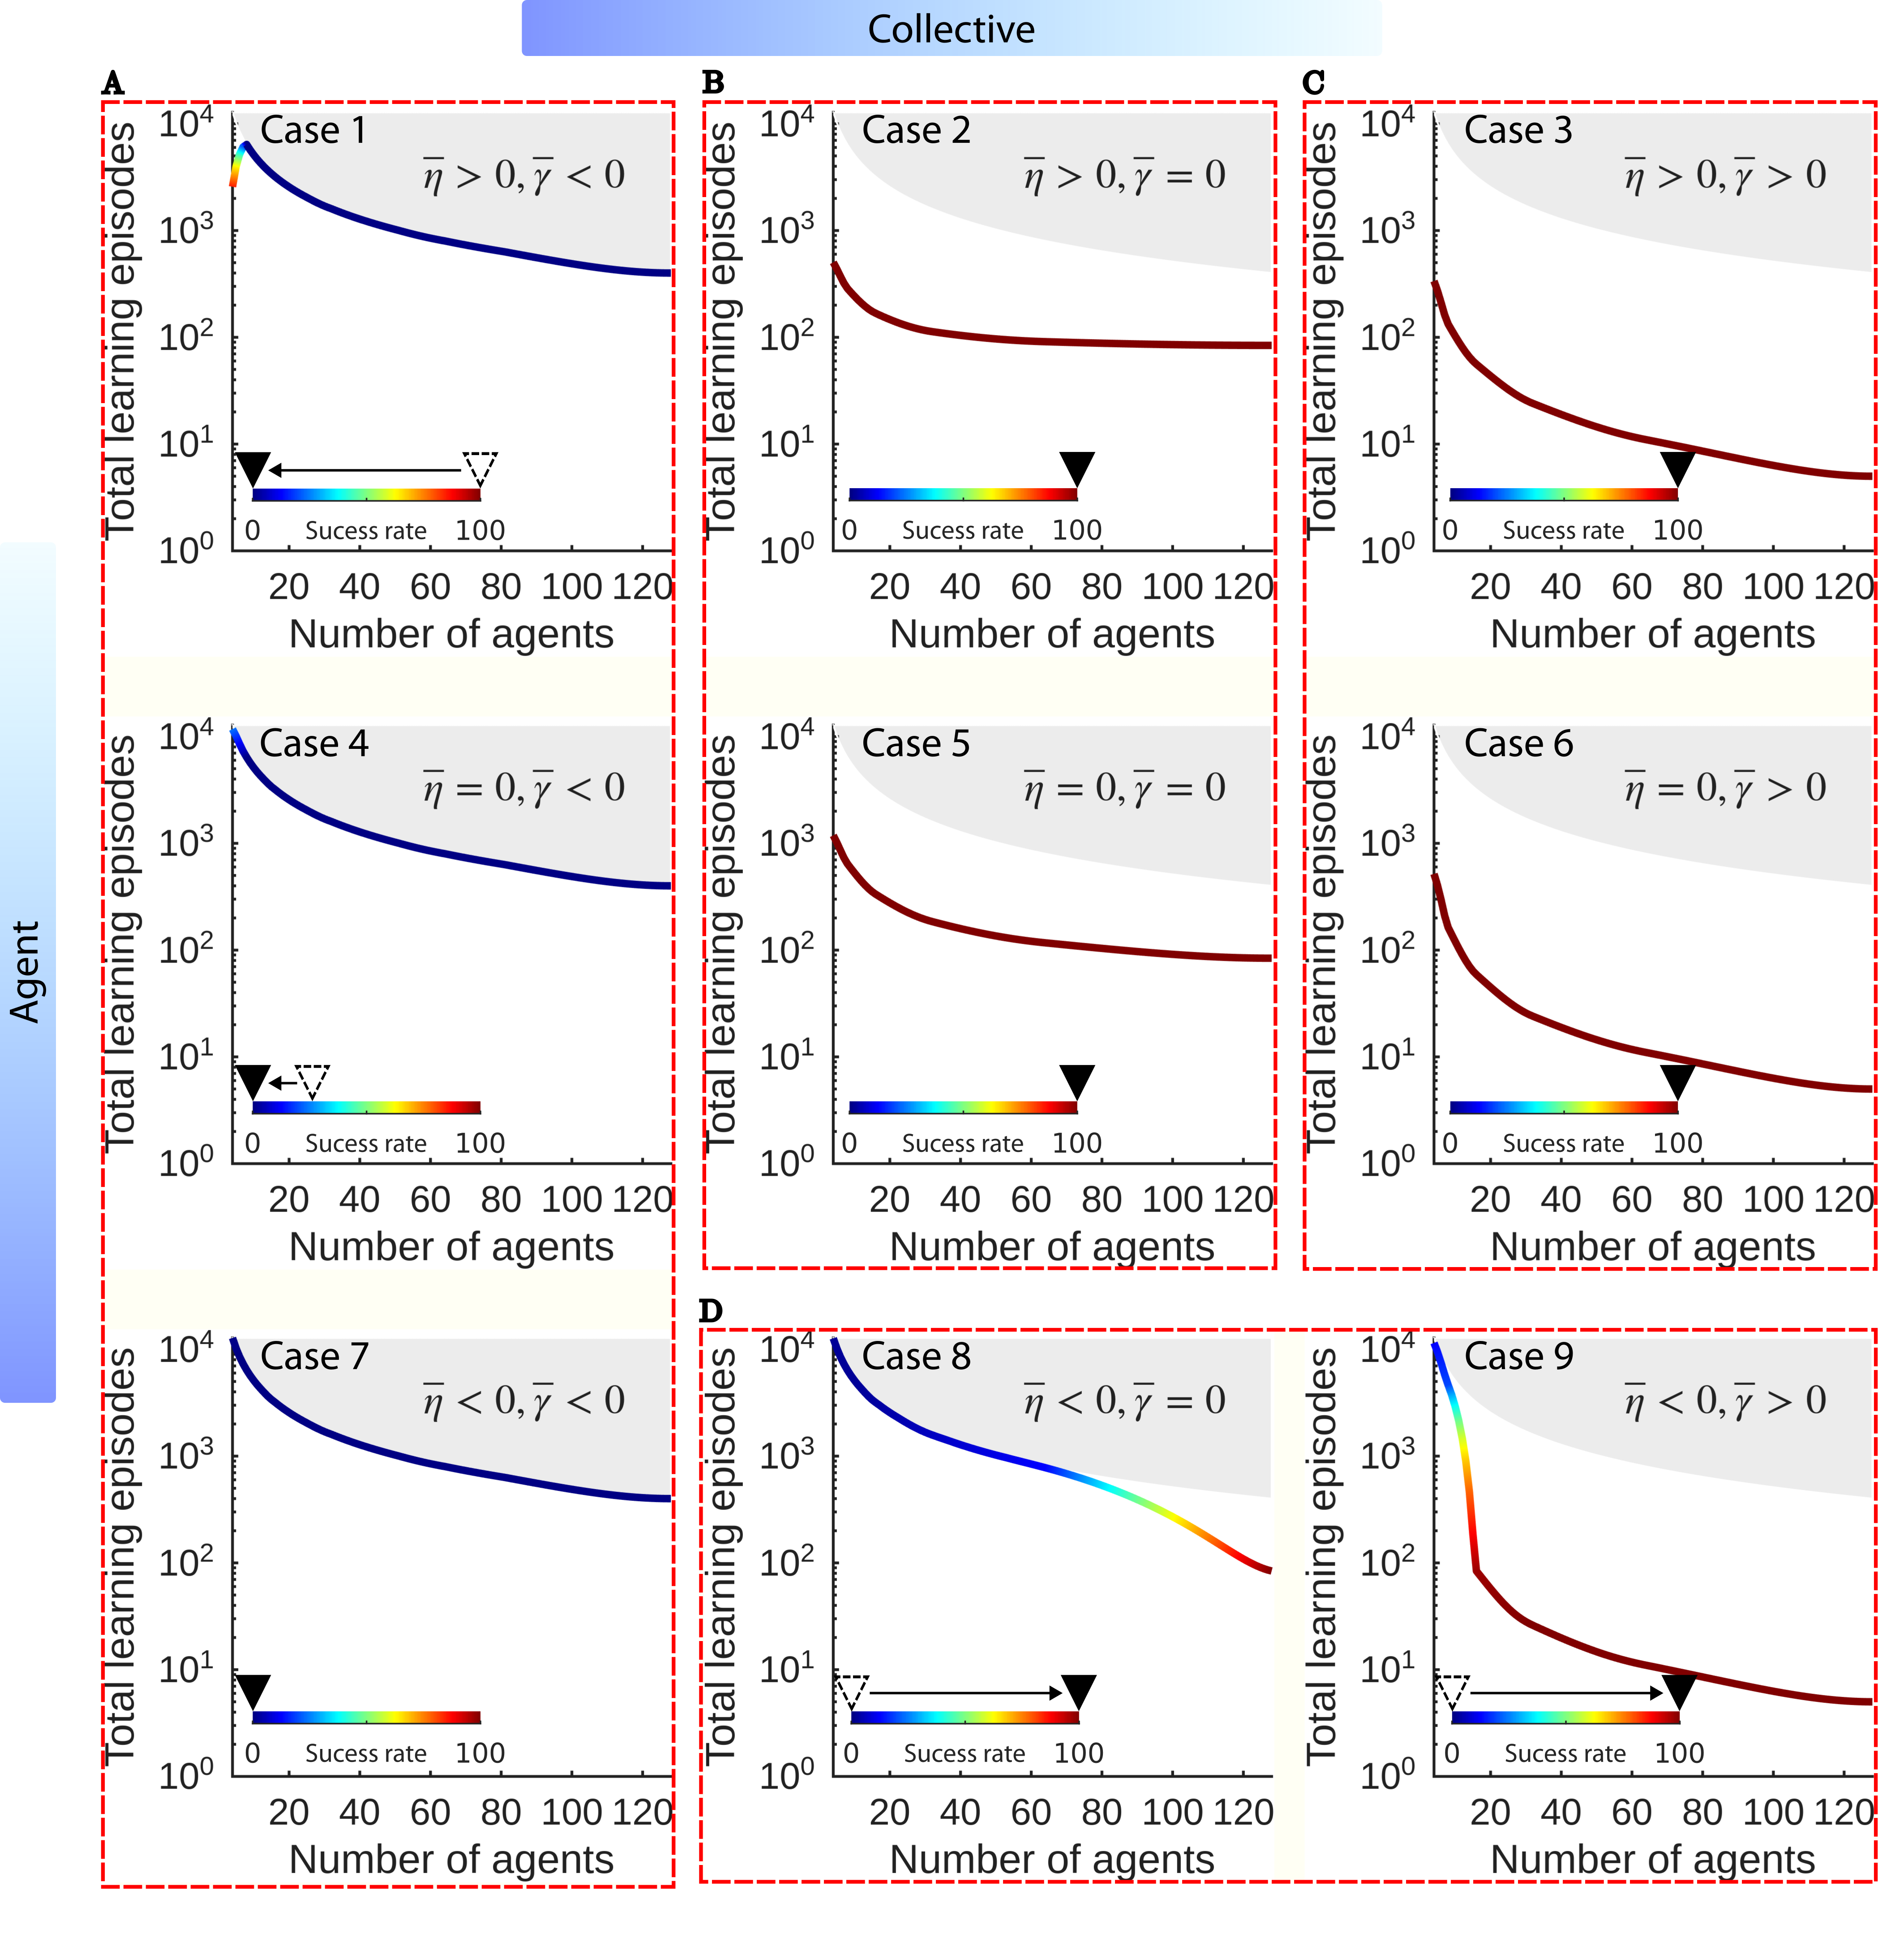
\includegraphics[width=16cm]{collective_learning_cases.png}
	\caption[] {\label{fig:collective_learning_cases_revised} \textbf{Different behaviors exhibited by a \acl{cl} system.} Depending on the mean values of $ \eta $ and $ \gamma $, a robot collective will exhibit different performance in terms of total episodes and success rate. Four categories are apparent: (\textbf{A}) destructive, (\textbf{B}) canceling, (\textbf{C}) ideal, and (\textbf{D}) compensating network behavior.}
\end{figure*}

\begin{table}[t!]
	\centering
	\caption{\label{tab:cl_regimes_revised} Regimes of a \ac{cl} system.}
	\begin{tabular}{|l|p{11cm}|}
		\hline
		\textbf{Case} & \textbf{Description}\\
		\hline
		Case 1 ($\bar{\eta} >0,~\bar{\gamma}<0$) & Agent accumulates knowledge, collective destroys knowledge. \\
		Case 2 ($\bar{\eta} >0,~\bar{\gamma}=0$) & Agent accumulates knowledge, collective corrupts knowledge.\\
		Case 3 ($\bar{\eta} >0,~\bar{\gamma}>0$) & Agent and collective accumulate knowledge.\\
		Case 4 ($\bar{\eta} =0,~\bar{\gamma}<0$) & Agent erratically accumulates knowledge, collective destroys knowledge.\\
		Case 5 ($\bar{\eta} =0,~\bar{\gamma}=0$) & Agent and collective erratically accumulate knowledge.\\
		Case 6 ($\bar{\eta} =0,~\bar{\gamma}>0$) & Agent erratically uses previous knowledge, collective shares knowledge.\\
		Case 7 ($\bar{\eta} <0,~\bar{\gamma}<0$) & Agent and collective destroy knowledge.\\
		Case 8 ($\bar{\eta} <0,~\bar{\gamma}=0$) & Agent corrupts knowledge, collective erratically shares knowledge.\\
		Case 9 ($\bar{\eta} <0,~\bar{\gamma}>0$) & Agent destroys knowledge, collective accumulates knowledge (compensates).\\
		\hline	
	\end{tabular}
\end{table}

The parameters $\bar{\eta}$ and $\bar{\gamma}$ define the behavior of a \ac{cl} system. $\bar{\eta}$ quantifies the quality of individual learning from prior knowledge, while $\bar{\gamma}$ characterizes the effectiveness of knowledge exchange between agents. Table~\ref{tab:cl_regimes_revised} and Fig.~\ref{fig:collective_learning_cases_revised} show nine characteristic regimes. These can be grouped into four broader categories: (\textbf{A}) \textbf{destructive}, where the network undermines learning; (\textbf{B}) \textbf{canceling}, where network effects lead to mediocre performance; (\textbf{C}) \textbf{ideal}, where individual and collective learning are mutually reinforcing; and (\textbf{D}) \textbf{compensating}, where a strong network makes up for weak individual learners. The performance plots show that successful learning in a collective is highly dependent on effective inter-agent connectivity, as seen in cases 8 and 9, where a large enough collective can succeed even with poor individual learners.

\paragraph*{A smart factory case study}
\begin{figure*}[t!]
	\centering
	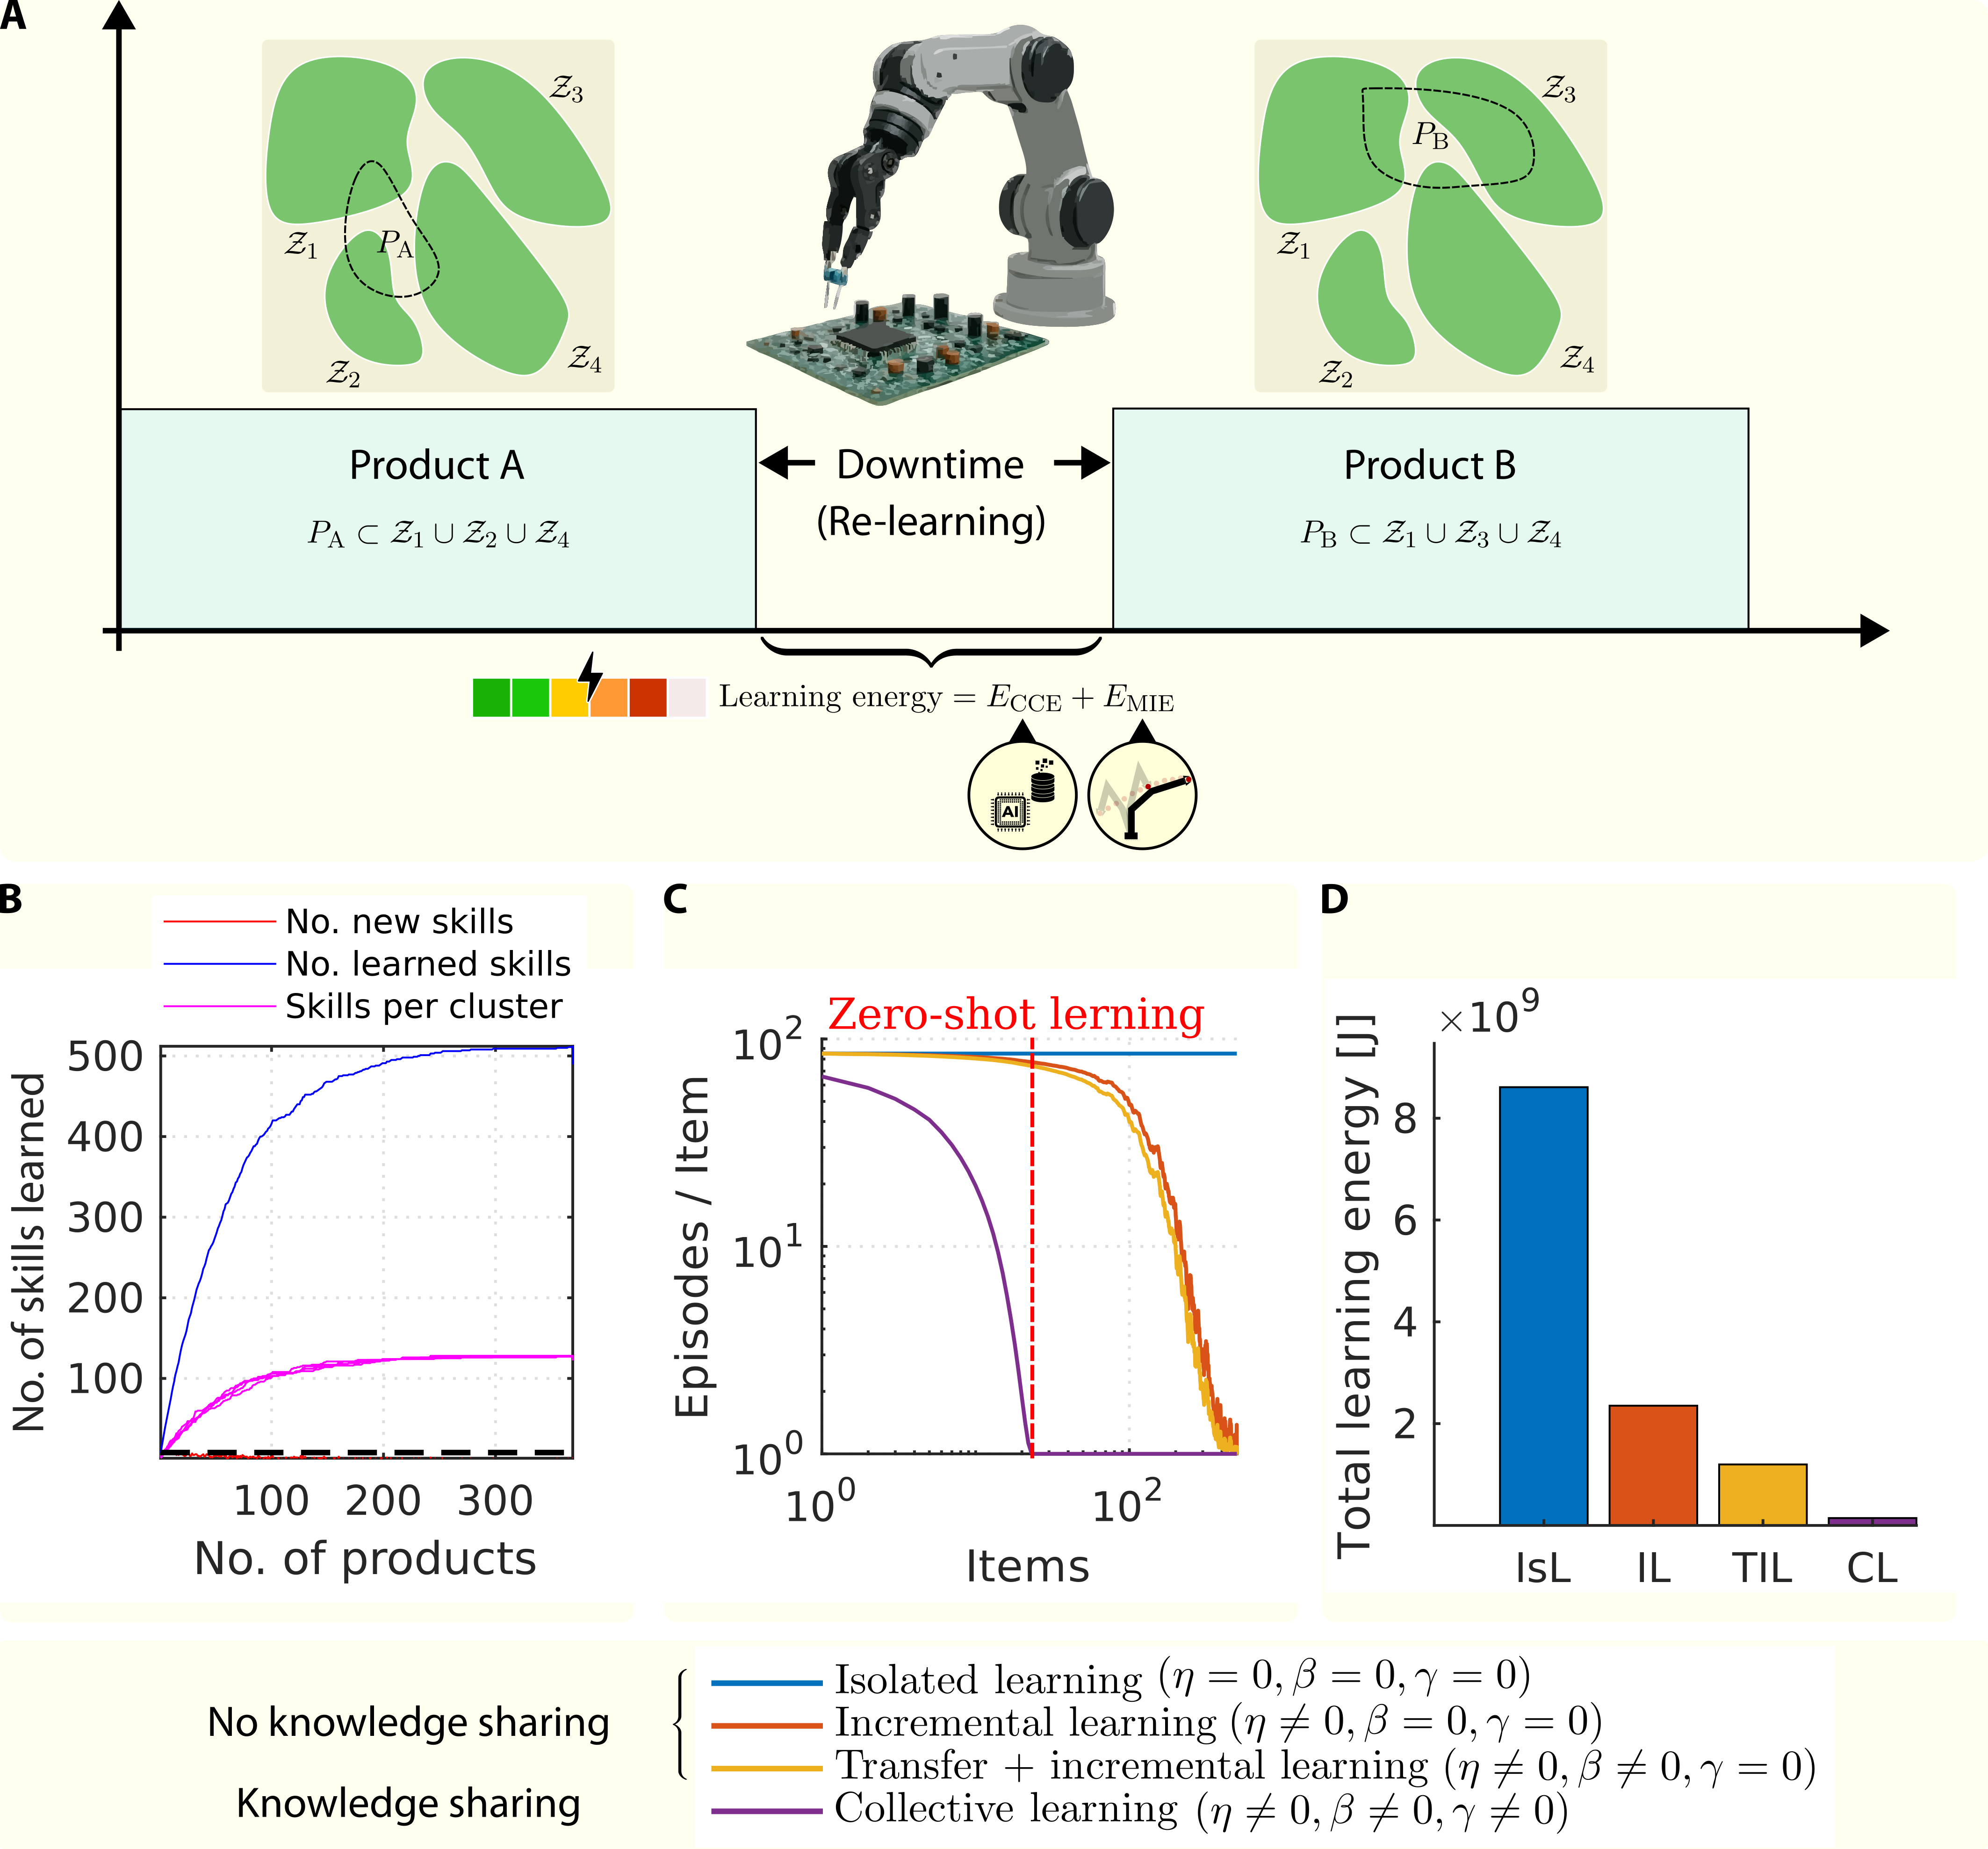
\includegraphics[width=16cm]{smart_factory_case_study.png}
	\caption[] {\label{fig:smart_factory_case_study_revised} \textbf{Smart sensor manufacturing.} {\textsc{Top}: A factory manufactures a new smart sensor each shift. During downtime, a robot collective learns the new skills required. \textsc{Bottom}: Learning episodes per product (left) and total learning energy (right) are shown.}}
\end{figure*}

We simulate a smart factory where a collective of $N_\mathrm{r} = 8$ robots learns skills to manufacture new smart sensors. The goal is to minimize the changeover downtime by learning the required skills as fast as possible. The power per episode is $P_0 = P_\text{BEE} + P_\text{MIE} + P_\text{CCE}$. We assume $P_\text{BEE} \approx \unit[40]{W}$ for a modern cobot, $P_\text{MIE} \approx \unit[300]{W}$, and $P_\text{CCE} \approx \unit[1416]{W}$ based on cloud computing for ML tasks \cite{Strubell2019EnergyPolicyConsiderations}. With an episode time of $\Delta t = 60$s, the energy per episode is $e_0 \approx 105~\text{kJ}$.

Fig.~\ref{fig:smart_factory_case_study_revised} (\textsc{Bottom}) shows that with \ac{cl}, after about 20 products, new skills are learned almost instantaneously (zero-shot). Compared to other paradigms like \ac{isl}, \ac{il}, and \ac{til}, \ac{cl} dramatically reduces the number of learning episodes. This is because \ac{cl} allows agents to benefit from the shared knowledge of the entire collective, not just their own experience. As a result, the total energy required for \ac{cl} is only about 10\% of that required by the next best paradigm, \acl{til}.

\section*{Discussion}\label{sec:discussion_revised}
\begin{figure*}[t!]
	\centering
	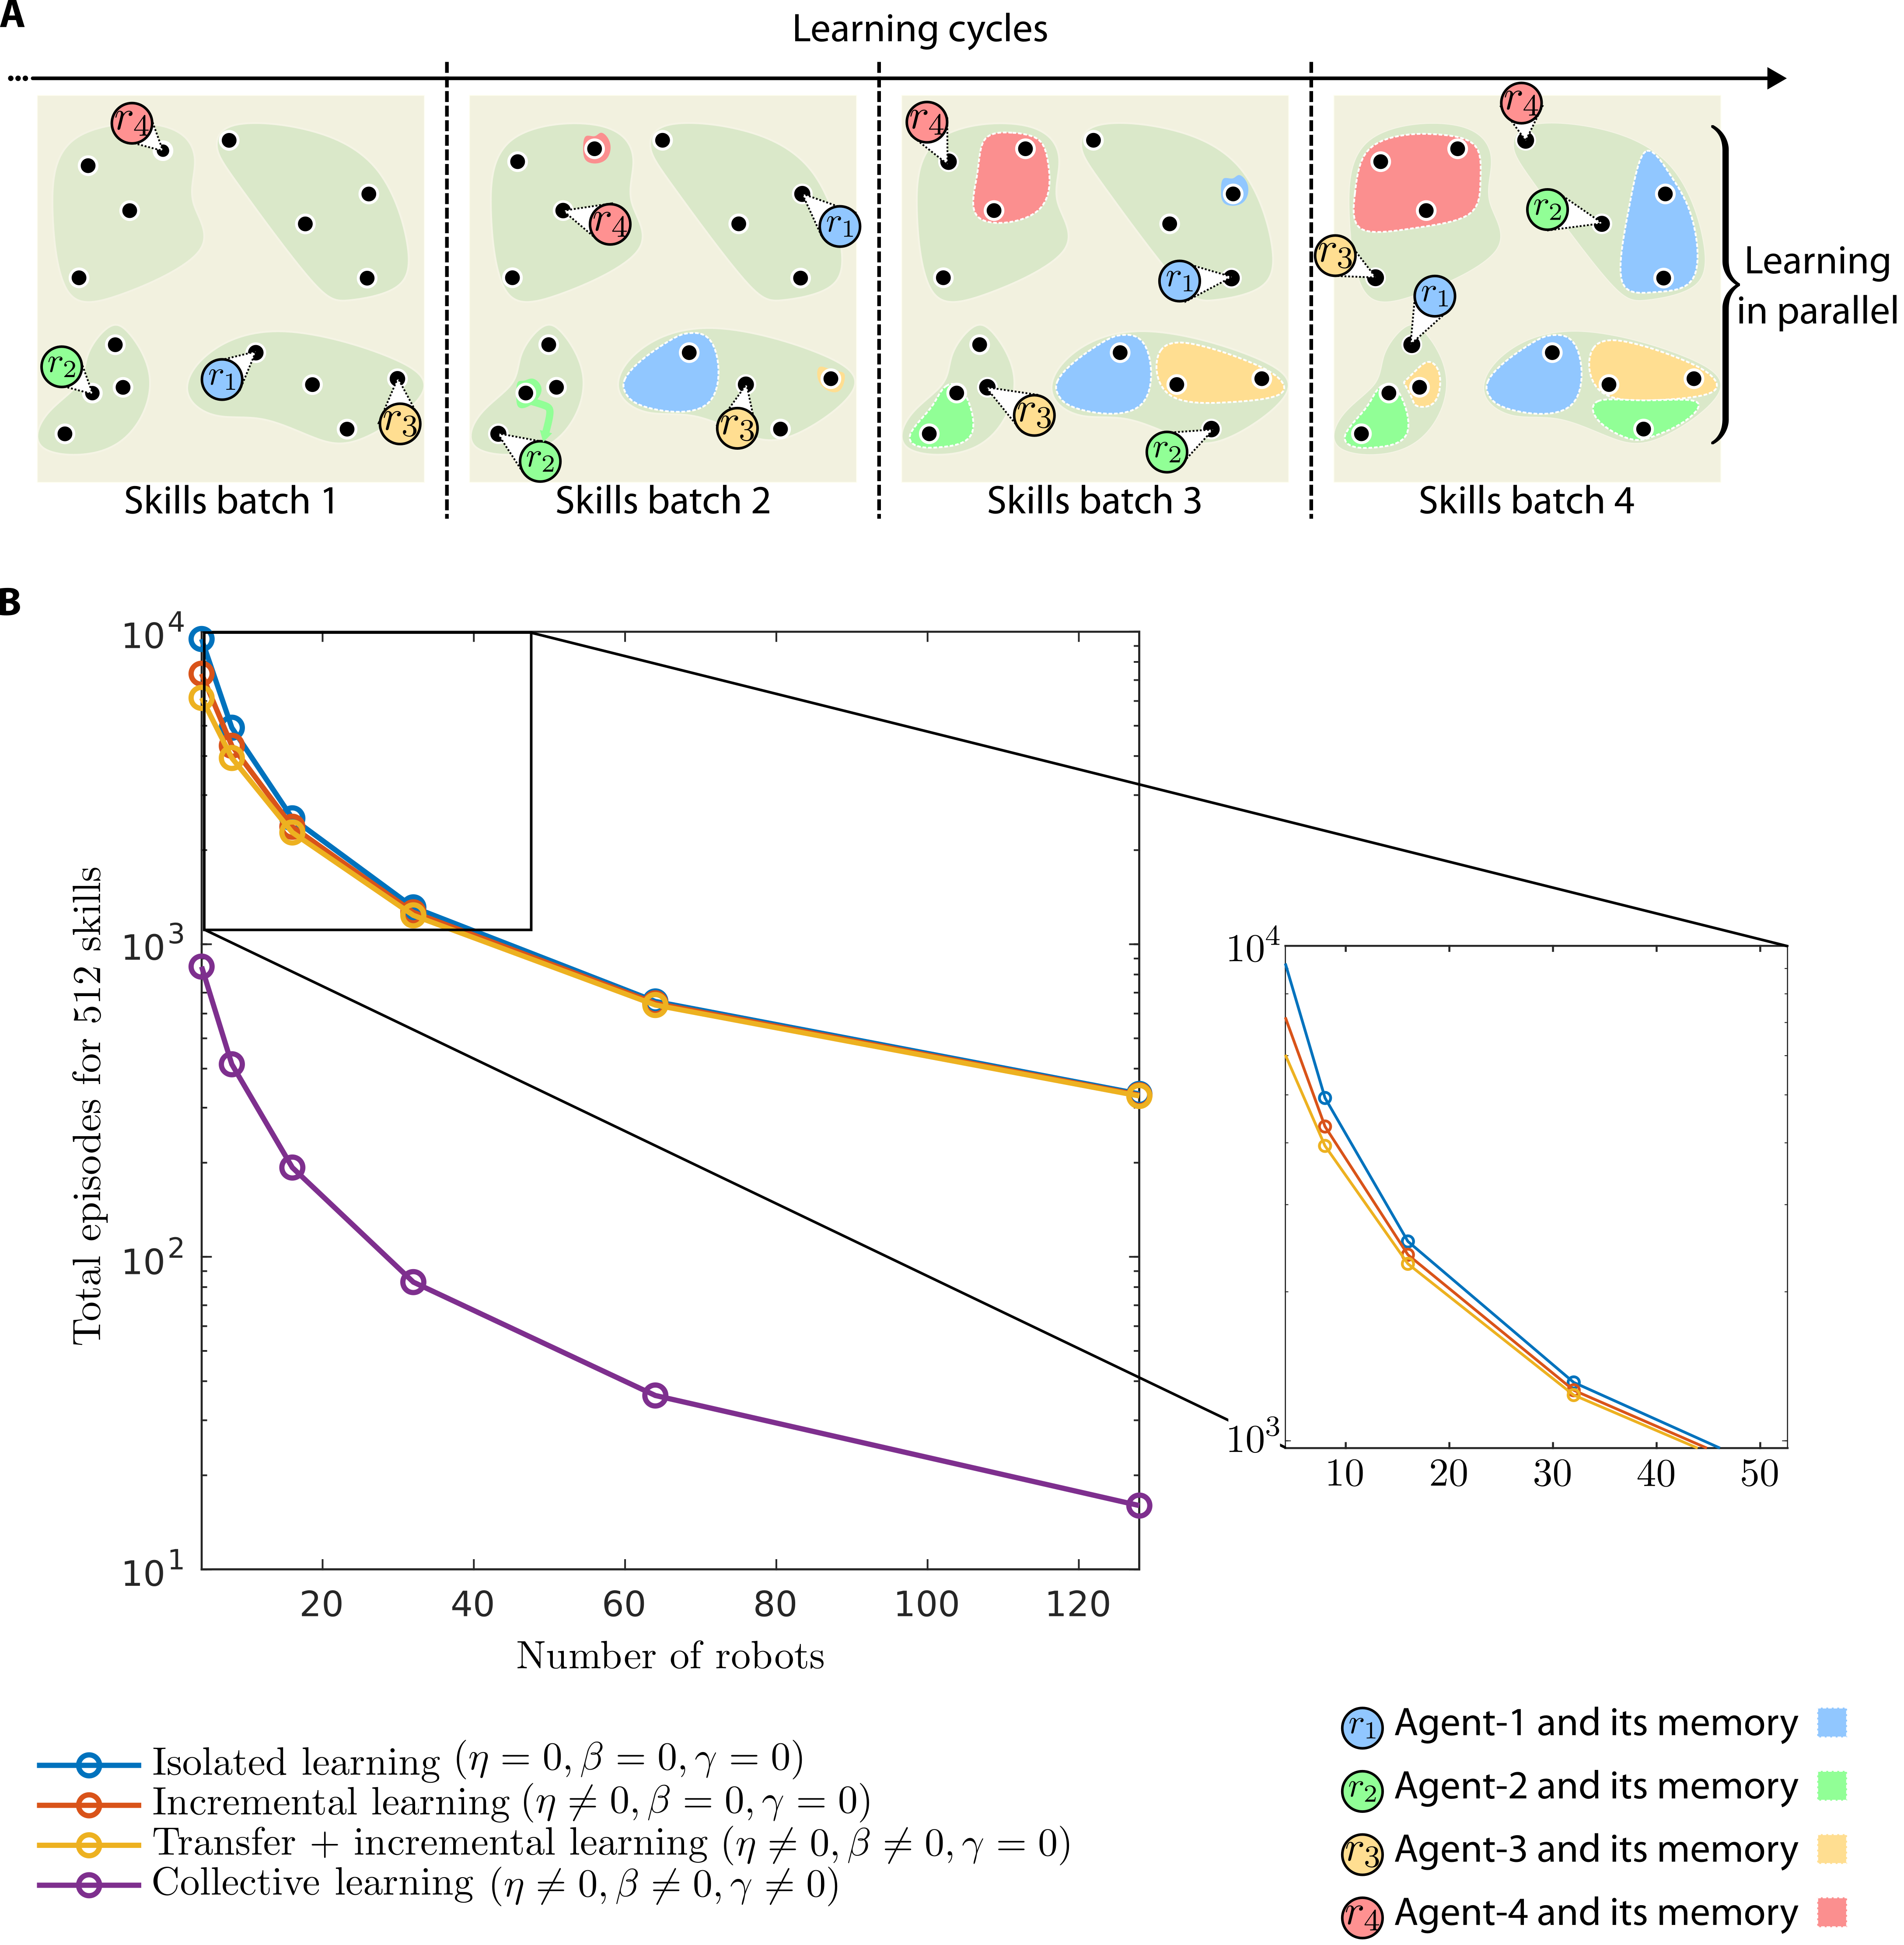
\includegraphics[width=16cm]{learning_paradigms_and_size_of_collective.png}
	\caption[] {\label{fig:learning_paradigms_and_size_of_collective_revised} \textbf{Effect of collective size on total learning episodes.} {\textsc{Top}: In classical paradigms, knowledge is split among agents, reducing available knowledge per agent as the collective grows. \textsc{Bottom}: As the number of agents increases, classical paradigms degrade towards \acl{isl}. In contrast, \acl{cl} leverages the number of robots to exponentiate learning.}}
\end{figure*}

\paragraph*{Splitting knowledge vs. sharing knowledge}
Fig.~\ref{fig:learning_paradigms_and_size_of_collective_revised} shows how the number of robots $N_\mathrm{r}$ affects the total episodes needed to learn all skills. In paradigms like \ac{il} and \ac{til}, as more robots join, the total pool of knowledge is fragmented among them. Each robot learns fewer skills, so there is less knowledge to transfer, and performance degrades towards that of \ac{isl}. In contrast, \ac{cl} thrives as the number of agents increases. The shared knowledge pool grows faster, leading to exponential improvements in learning efficiency and a reduction in total energy consumption.

\paragraph*{On the parameters of the collective system}
The model parameters $(\alpha, \beta, \gamma, \eta)$ are influenced by factors like communication quality and agent capabilities. The system's stability and performance depend on these parameters. A key finding is that the ideal regime for \ac{cl}, where it vastly outperforms other paradigms, corresponds to parameter ranges that are plausible in real-world applications, highlighting the practical promise of this approach.

\paragraph*{Developing collective learning to address the energy challenges of \ac{eai}}
\begin{figure}[!t]
	\centering
	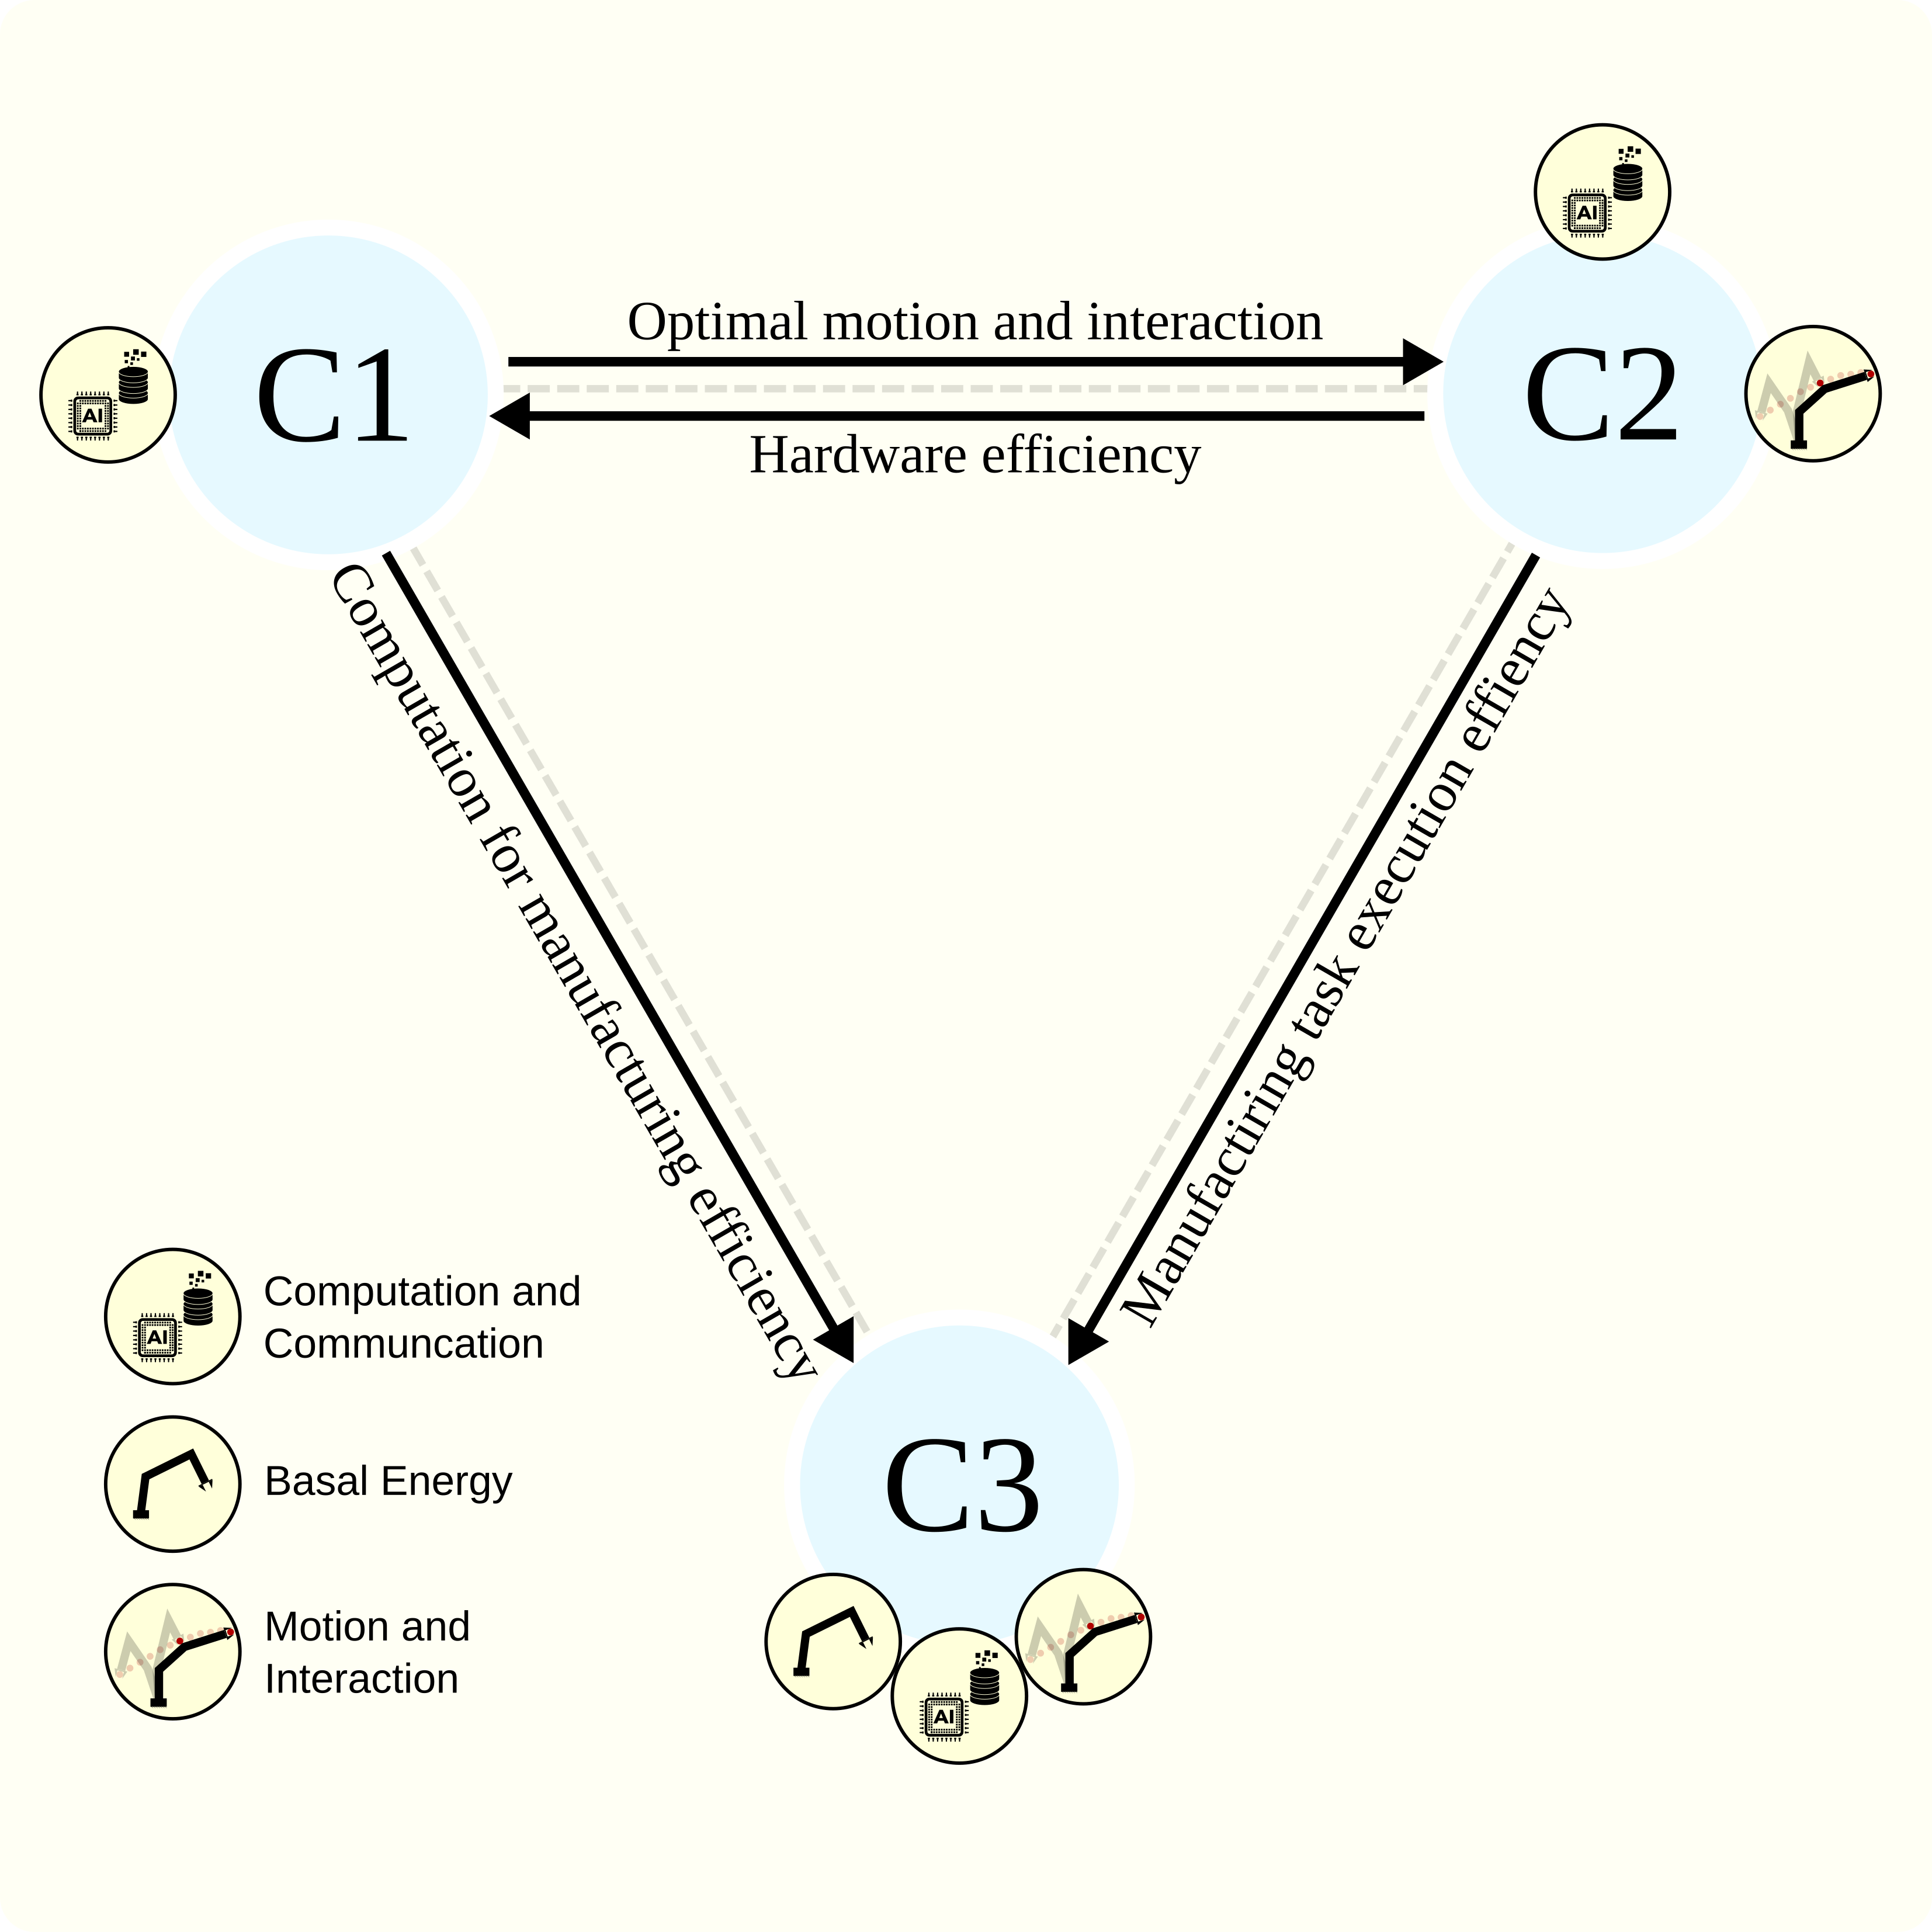
\includegraphics[width=0.45\textwidth]{fig/grand_challenges_connections.png}
	\caption{\textbf{Interconnection between challenges C1, C2, and C3.}}
	\label{fig:challengesConnected_revised}
\end{figure}
As shown in Fig.~\ref{fig:challengesConnected_revised}, collective learning addresses the key energy challenges in \ac{eai}. For Challenge C1 (AI infrastructure energy), \ac{cl} reduces computational load ($E_\text{CCE}$) by focusing on efficient knowledge sharing rather than brute-force retraining. This could shift data center usage from computation to storage and querying. For Challenge C2 (robot operational energy), \ac{cl} reduces learning time, which in turn cuts down on basal ($E_\text{BEE}$) and motion-related ($E_\text{MIE}$) energy consumption. Progress on C1 and C2 naturally helps with C3 (manufacturing energy) by improving the efficiency and lifespan of robotic systems, which can be further enhanced through recycling.

\paragraph*{Closing remarks}
The proliferation of AI and robotics necessitates a focus on sustainable energy consumption. We have argued that mitigating energy use in \ac{eai} requires a paradigm shift towards the systematic sharing and aggregation of knowledge. Efficient robotic learning requires algorithms to be sample-efficient, generalizable, compositional, and capable of incremental learning \cite{Kaelbling2020foundationefficientrobot}. The \acl{cl} paradigm inherently supports these attributes by leveraging networked communication. Our simulations show that without true inter-agent knowledge exchange, energy demands scale inefficiently with the number of agents. In contrast, \ac{cl} demonstrates superior performance and energy efficiency, especially as the collective grows. While the algorithms to fully realize \ac{cl} are still under development, its principles are also applicable to \ac{dai}, for instance in federated learning and the fine-tuning of foundation models. We hope this work catalyzes further research into collective learning to build more scalable, adaptable, and energy-efficient AI systems.

\section*{Methods}\label{sec:methods_revised}
\paragraph*{Modeling the dynamics of skill knowledge}
The complexity $c_j$ of a skill $s_j$ is the number of trial episodes needed to learn it. We assume that the power $P_0$ per episode and the time per episode $\Delta t$ are approximately constant. Thus, the energy to learn a skill is proportional to its complexity. Skills are grouped into clusters $\mathcal{Z}_k$ based on similarity. We assume that knowledge from learned skills in a cluster, $\mathcal{\zeta}_k$, can expedite the learning of new skills in that same cluster.

We model the remaining knowledge to be learned for a skill $s_{j,k}$ as $\bar{\sigma}_{j,k}(n) \in [0,1]$. This function decreases as an agent learns. An idealization of this process is a first-order dynamical system:
\begin{definition}
The remaining knowledge function $\bar{\sigma}_{j,k}$ is modeled as:
	\begin{equation}\label{eq:simple_knowledge_dynamics_revised}
		\dot{\bar{\sigma}}_{j,k}\left(n\right)=\begin{cases}
			-f_{j,k} \left(N_{\zeta_k} \right) \bar{\sigma}_{j,k}\left(n\right), & \epsilon < \bar{\sigma}_{j,k}\left(n\right) < 1, \\
			0, & \text{otherwise}.
		\end{cases}
	\end{equation}	
\end{definition}
where $N_{\zeta_k}$ is the number of already learned skills in the cluster. The solution is $\bar{\sigma}_{j,k}(n) = g_{j,k}(N_{\zeta_k}) e^{-f_{j,k}(N_{\zeta_k}) n}$, where $g(\cdot)$ models the initial remaining knowledge and $f(\cdot)$ models the learning rate.

\paragraph*{Knowledge sharing under different learning paradigms}
We assume a system with comparable \ac{eai} agents learning skills that are ordered and segregated by similarity. We consider four paradigms:
\begin{itemize}
    \item \textbf{\Acl{isl}}: Learns every skill from scratch.
    \item \textbf{\Acl{il}}: Benefits from knowledge of skills within the same cluster \cite{Lesort2020Continuallearningrobotics}.
    \item \textbf{\Acl{tl}}: Uses knowledge from different source clusters for learning in a target cluster \cite{Hosna2022Transferlearningfriendly,Jaquier2023TransferLearningRobotics}.
    \item \textbf{\Acl{cl}}: Agents dynamically develop a common body of knowledge through networked interactions, sharing experience both vertically (from past knowledge) and horizontally (from concurrent experience) \cite{Garavan2012CollectiveLearning}.
\end{itemize}

\paragraph*{\textbf{\Acl{cl}}}
In our model of \ac{cl}, the dynamics of the remaining knowledge for an agent exchanging information with a set of neighbors $\mathcal{N}$ is given by:
\begin{equation}\label{eq:collective_knowledge_dynamics_revised}
	\dot{\bar{\sigma}}^{(\text{CL})}_{j,k} =
		\left[-\alpha \left( \frac{\eta \kappa + 1}{1 - \xi_k} \right)  - \sum\limits_{l \in \mathcal{N}(j)} \bar{\xi}_{j,l} \gamma_{j,l} d(\bar{\sigma}_j,\bar{\sigma}_l)\right] \bar{\sigma}^{(\text{CL})}_{j,k},
\end{equation}
for $\epsilon < \bar{\sigma}_{j,k} < 1$. Here, $\kappa$ is the total number of skills learned by the collective. The parameters are: $\alpha$ (base learning rate), $\eta$ (intra-cluster knowledge exchange factor), $\gamma$ (inter-agent knowledge exchange factor), $\xi_k$ (inter-cluster knowledge transfer factor), and $d(\cdot,\cdot)$ (a function weighting the relevance of shared knowledge). Table~\ref{tab:learning_paradigms_expressions_revised} summarizes the specific forms of the dynamic equations for each learning paradigm.

\begin{table}[!t]
	\caption{The dynamics of the learning paradigms.\label{tab:learning_paradigms_expressions_revised}}
	\centering
	\begin{adjustbox}{width=\textwidth}
		\begin{tabular}{|l||c|c|c|c|}
			\hline
			\textbf{Learning paradigm} & \textbf{\ac{isl}} & \textbf{\ac{il}} & \textbf{\ac{til}} & \textbf{\ac{cl}} \\
			\hline\hline
			Rate $f_{j,k}\left(\cdot \right)$  & $-\alpha$ & $-\alpha\left(\eta \kappa + 1 \right)$ & $-\alpha \left( \frac{\eta \kappa + 1}{1 - \xi_k} \right)$ & $  -\alpha \left( \frac{\eta \kappa + 1}{1 - \xi_k} \right)  - \sum_{l \in \mathcal{N}(j)}\bar{\xi}_{j,l}\gamma_{j,l}d(\bar{\sigma}_j,\bar{\sigma}_l)$ \\
			\hline
			Initial condition $g_{j,k}\left(\cdot \right)$ & $1$ & $e^{-\delta \kappa}$ & $(1-\xi_k) e^{-\delta \kappa}$ & $(1-\xi_k) e^{-\delta \kappa} $ \\
			\hline
		\end{tabular}
	\end{adjustbox}
\end{table}

%================= ACKNOWLEDGMENTS, FUNDING, ETC. =================
\section*{Acknowledgments}
\textbf{Acknowledgments:} We thank Carlos Magno C. O. Valle for his feedback and support.
\textbf{Funding:} The authors acknowledge funding from the Alfried Krupp von Bohlen und Halbach Foundation.
\textbf{Author contributions:} S.H. developed the core concept. S.H. and F.D.L. developed the mathematical framework. F.D.L. conducted experiments and analyzed data. F.D.L. and S.H. interpreted results and wrote the manuscript. All authors read the paper.
\textbf{Competing interests:} The authors declare no competing interests.
\textbf{Data and materials availability:} All necessary data are in the main manuscript or Supplementary Materials. Address requests for additional materials to S.H.

%================= SUPPLEMENTARY MATERIALS AND REFERENCES =================
\beginsupplement
\newpage
\section*{Supplementary Materials}
\label{sec:supplementary_materials_revised}
% ===================================================================================================
%                                                 |                                                 |
%                                                 |                                                 |
% -------------------------------------------- SECTION ---------------------------------------------|
%                                                 |                                                 |
%                                                 |                                                 |
% ===================================================================================================
\section{Materials and Methods}\label{sec:materials_and_methods}

% ===================================================================================================
\subsection{Episodic energy and time requirements}\label{sec:power_per_episode}
% ---
\begin{figure}[!h]
	\centering
	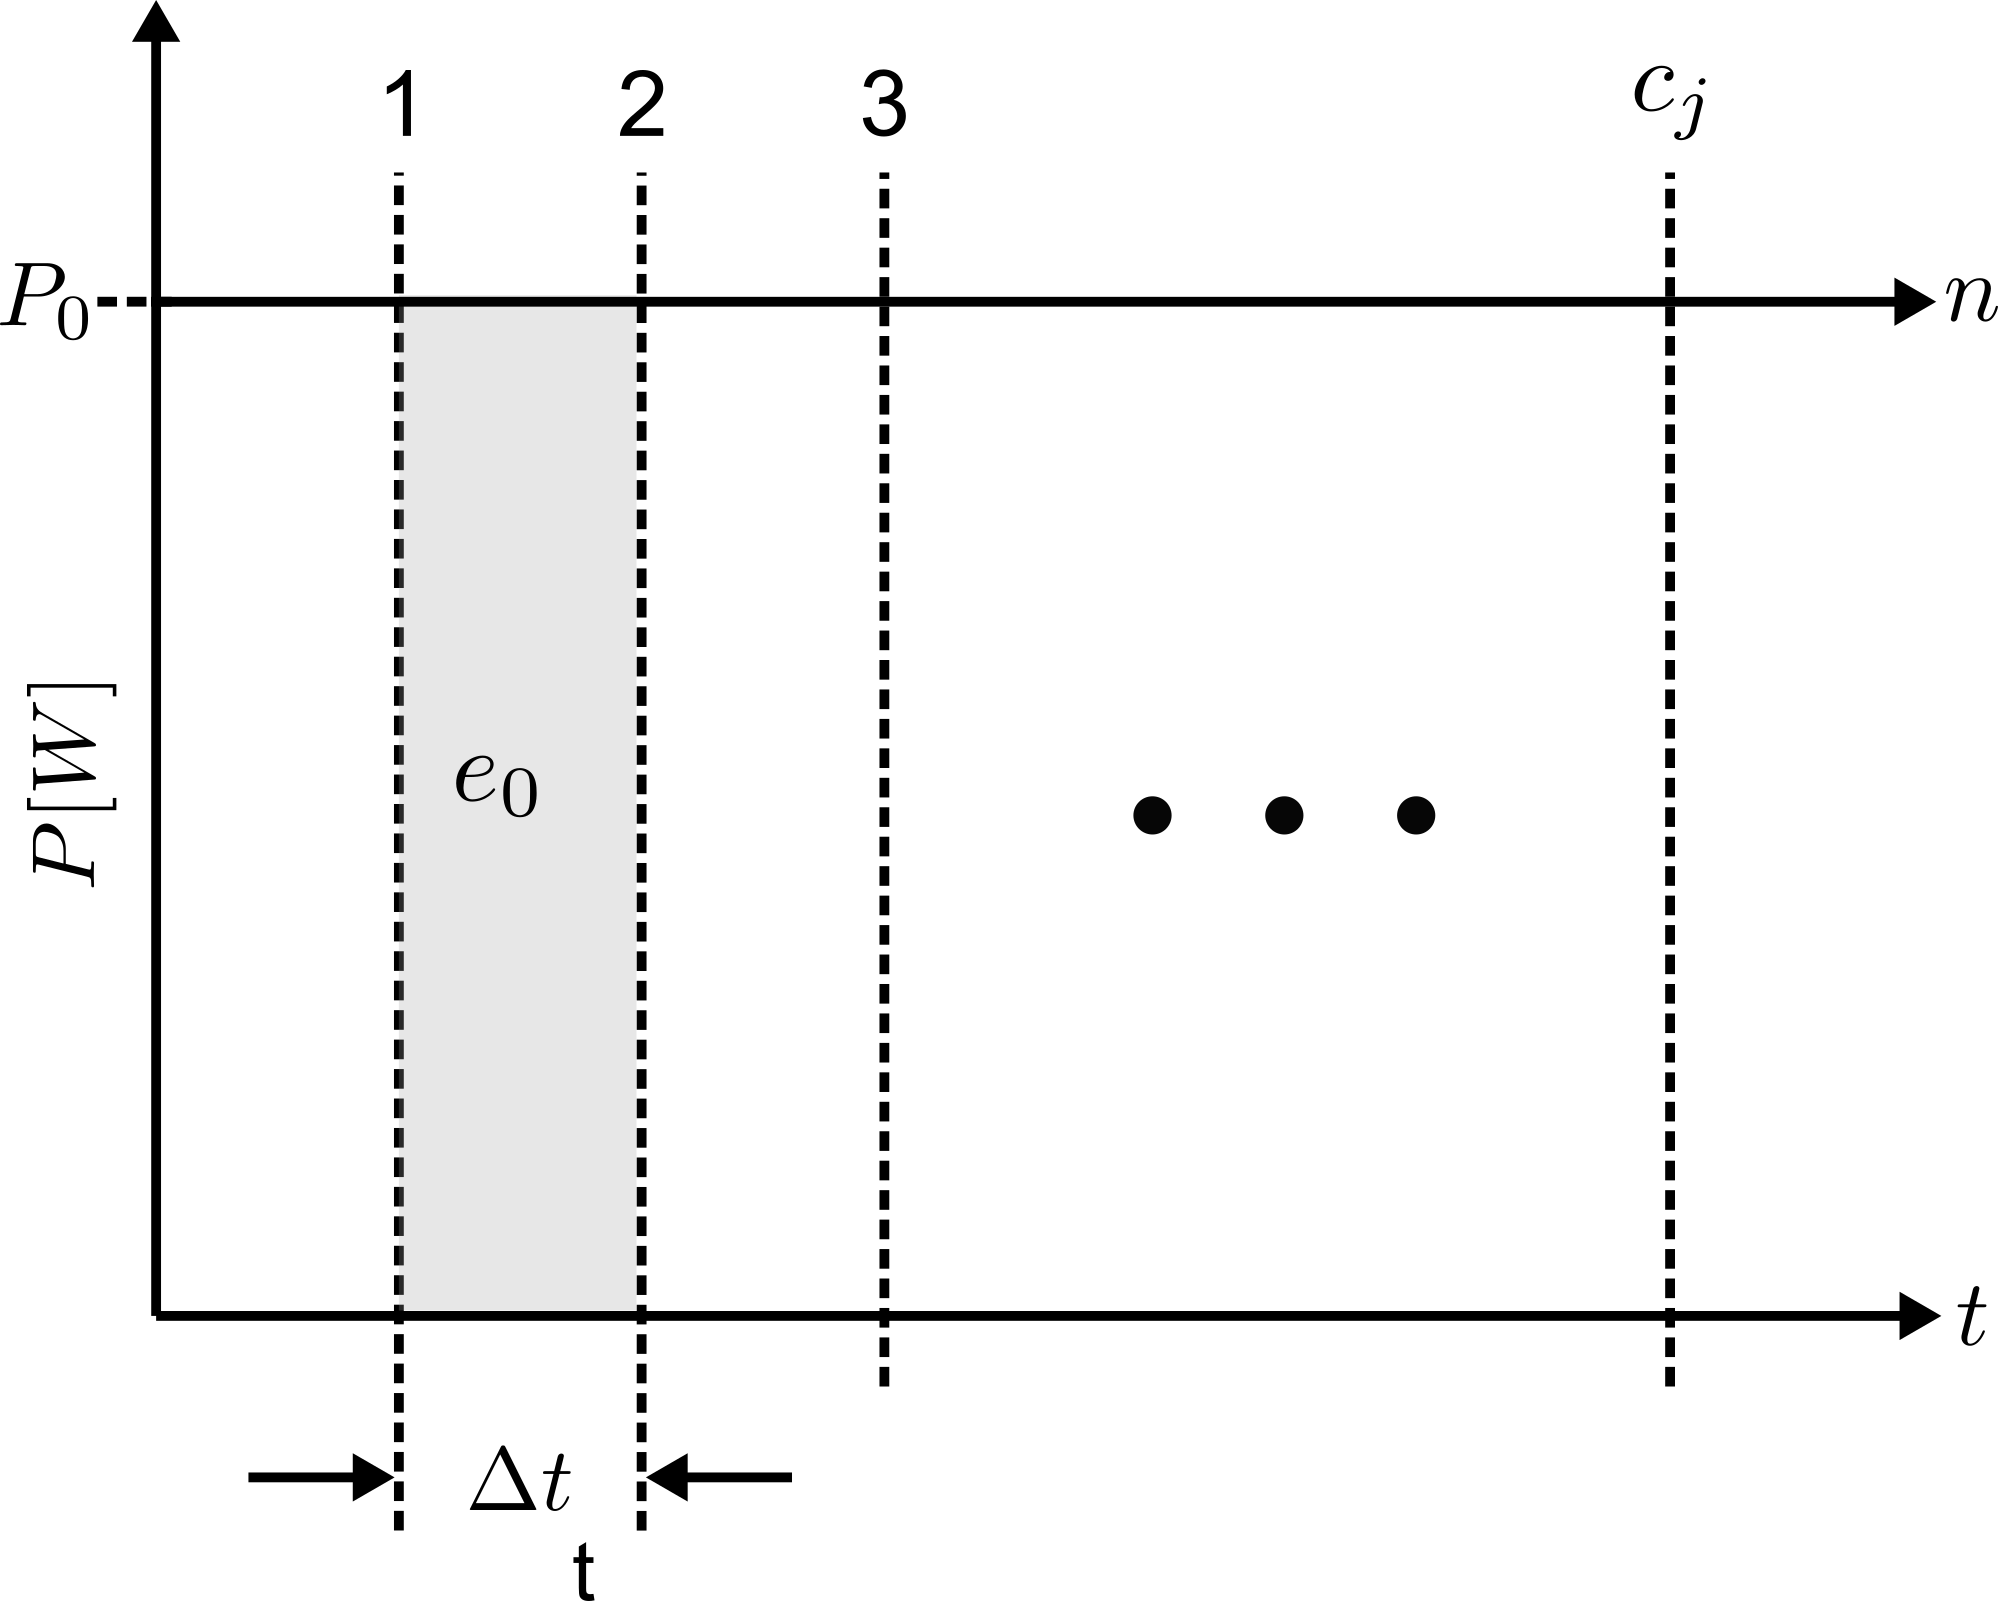
\includegraphics[width=0.45\textwidth]{fig/power_per_episode.png}
	\caption{Power consumption per episode.}
	\label{fig:power_per_episode}
\end{figure}
% ---
\paragraph{Energy requirements.}
Under Asm.~\ref{assumption:power_and_episode_time}, the energy consumption of the $n$-th episode $e_j(n)$ is the constant product
% ---
\begin{equation}\label{eq:energy_per_episode}
	e_j(n) = \underbrace{P_0 \Delta t}_{\text{constant}} = e_0.
\end{equation}
% ---
Consequently, the energy consumed by a robot learning a skill $ s_j $ is directly proportional to the skill complexity $c_j$; i.e.
% ---
\begin{equation}\label{eq:energy_per_skill}
	E_j =\sum_{n=1}^{c_j} e_j(n) = e_0c_j.
\end{equation}
% ---
The energy spent on learning $\mathcal{S}$ under the absence of knowledge transfer is
% ---
\begin{equation}\label{eq:total_energy}
	E_{\mathcal{S}} = \sum_{j=1}^{{N_{\mathcal{S}}}} E_j = e_0 \sum_{j=1}^{{N_{\mathcal{S}}}} c_j%N_{\mathcal{T}} \cdot e_0 \cdot c_j 
\end{equation}
% ---
% ---------------------------------------------------------------------------------------------------
\paragraph{Time requirement.} Similarly, the total learning time $T_{\mathcal{S}}$ for a simple agent is
% ---
\begin{equation}\label{eq:total_time}
	T_{\mathcal{S}} = \Delta t \sum_{j=1}^{{N_{\mathcal{S}}}} c_j.
\end{equation}
% ---

% ===================================================================================================
\subsection{The different learning paradigms}\label{sec:types_of_learning}

% ---------------------------------------------------------------------------------------------------
\paragraph{Isolated Learning (IsL)} A robot performs IsL when it learns each skill in $\mathcal{Z}_k$ one after another from the ground up, disregarding the accumulating knowledge from already learned skills. In such a case the rate of convergence and the initial remaining knowledge for all skills are given by
% ---		
\begin{subequations}\label{eq:fg_isolated}
	\begin{alignat}{2}
		f_{j,k}\left(\cdot \right) &=  -\alpha \\
		g_{j,k}\left(\cdot \right) &= 1,
	\end{alignat}
\end{subequations}
% ---
where $ \alpha>0$ models the rate at which a robot in isolation learns any given skill. Relying on Asm.~\ref{assumption:agent_similarity} we can assign a value to $\alpha$ by using the fundamental complexity $c_0$ as follows
% ---
\begin{equation}\label{eq:isolated_learning_rate}
	\alpha = -\frac{1}{c_0}\text{log}(\epsilon).
\end{equation}
% ---
Since in isolated learning $c^{(IsL)}_{j,k} = c_0$, the trial episodes required by one single robot to learn the skills in the cluster $\mathcal{Z}_k$ is given by
% ---
\begin{equation}
	%	\begin{split}
		%		C^{(IsL)}_{k} &= \sum_{j=1}^{N_{\mathcal{Z}}} c^{(IsL)}_{j,k}= N_{\mathcal{Z}}  \cancelto{c_{0}}{c^{(IsL)}_{j,k}} = N_{\mathcal{Z}} c_0
		%	\end{split}
	C^{(IsL)}_{k} = \sum_{j=1}^{N_{\mathcal{Z}}} c^{(IsL)}_{j,k}= N_{\mathcal{Z}}  c^{(IsL)}_{j,k} = N_{\mathcal{Z}} c_0.
\end{equation}
%-- 
Similarly, the total trial episodes to learn the universe of skills is simply
% ---
\begin{equation}
	C^{(IsL)}_{\mathcal{S}} = N_\mathcal{K} N_{\mathcal{Z}} c_0.
\end{equation}
% ---

\textbf{Multi agent case.} Suppose that a batch of $m$ robots is used to learn the same number of skills in parallel in a given cluster $\mathcal{Z}_k$. Such a strategy only distributes equally the total number of episodes by the number of available robots; i.e.
% ---
\begin{equation}
	^{\lvert \lvert}C^{(IsL)}_k=  \overbrace{\frac{1}{m}C^{(IsL)}_k}^{\text{episodes per robot}}.
\end{equation}
% ---

% ---------------------------------------------------------------------------------------------------
\paragraph{\textbf{Incremental Learning (IL)}}
It corresponds to the continuous aggregation and exchange of knowledge from \emph{intra-cluster} skills. Referring back to Asm.~\ref{assumption:skill_clustering}, the knowledge from skills belonging to a cluster ${\mathcal{Z}_k}$ can be be leveraged by an agent in virtue of their significant similarity. As depicted in Fig.~\ref{fig:intra_skill_learning}, a robot ($r_1$ in this case) learns every skill in $\mathcal{Z}_1$ with a rate $\alpha$ ---the self loops--- but also retains and uses the acquired knowledge to learn subsequent skills. The effect of incremental learning on the knowledge collection rate can be modeled to be directly proportional to the number of learned skills as
% ---
\begin{equation}\label{eq:f_function_incremental}
	f_{j,k}\left(N_{\zeta_k}\right) = -\alpha\left(\eta N_{\zeta_k} + 1 \right), 
\end{equation}
% ---
where $\eta>0$ represents the efficiency of knowledge exchange from $\zeta_k$ to $s_{j,k}$. Different potential models might be used to model the depletion of the initial remaining knowledge represented by $g_{j,k}\left(N_{\zeta_k}\right)$, e.g. a linear decay rate, our expectation is that, under the assumption that a learning strategy involving the ordering of skills according to similarity and their balanced distribution in the different clusters, $g_{j,k}\left(N_{\zeta_k}\right)$ might naturally resemble an exponential decay that is strongly dependent on $N_{\zeta_k}$. Such considerations motivate our choice of the following function
% ---
\begin{equation}\label{eq:g_function_incremental}
	g_{j,k}\left(N_{\zeta_k}\right) = e^{-\delta N_{\zeta_k}},
\end{equation}
%---
again with a factor $\delta>0$ controlling the rate at which the exponential converges. Similar to $\alpha$, using Asm.~\ref{assumption:cluster_size} $\delta$ can be defined as 
% ---
\begin{equation}\label{eq:delta}
	\delta = -\frac{1}{N_\mathcal{Z}}\text{log}(\epsilon).
\end{equation}
% ---
Essentially, such choice of $\delta$ implies that the remaining knowledge in a cluster after seeing all its skills is negligible. Via the exchange factors $(\eta,\delta)$, in incremental learning the knowledge about every new skill gets gradually increased by leveraging previous knowledge, resulting in
% ---
\begin{equation*}\label{eq:remaining_knowledge__IL}
	\bar{\sigma}^{(IL)}_{i,j}(n) = e^{-\alpha  \left(\eta N_{\zeta_k}+1\right) n} e^{-\delta N_{\zeta_k}}.
\end{equation*}
% ---
As the complexity $c_{j,k}$ of a skill can also be interpreted as the number of trial episodes required for the remaining knowledge to go below a threshold $\epsilon$; i.e.
% ---
\begin{equation*}
	\bar{\sigma}^{(IL)}_{i,j}(n) \Big \rvert_{n \ge c^{(IL)}_{j,k}} \leq \epsilon.
\end{equation*}
% ---
Then, under this scheme the complexity $c^{(IL)}_{j,k}$ to learn a new is skill in the cluster results in
% ---
\begin{equation}\label{eq:complexity_IL}
	c^{(IL)}_{j,k} = -\frac{\text{log}(\epsilon) - \text{log}\left(\bar{\sigma}^{(IL)}_{j,k}(0)\right)}{\alpha (\eta N_{\zeta_k}+ 1)} = -\frac{\text{log}(\epsilon) + \delta N_{\zeta_k}}{\alpha (\eta N_{\zeta_k}+ 1)}  .
\end{equation}
% ---
The total number of trial episodes $ C_k $ that an agent following an incremental learning strategy needs to learn the $N_{\mathcal{Z}_k}$ skills in a cluster $ \mathcal{Z}_k $ is given by
% ---
\begin{align}\label{eq:total_episodes_incremental}
	\begin{split}
		C^{(IL)}_k &= \sum^{N_{\mathcal{Z}}}_{j=1} c^{(IL)}_{j,k}.
	\end{split}
\end{align}
% ---

\textbf{Multi-agent case.} If $m$ robots are used in parallel to divide the load of learning the tasks then
% ---
\begin{align}
	\begin{split}
		{}^{\lvert \rvert}C^{(IL)}_k &= \sum^{\frac{N_{\mathcal{Z}}}{m}}_{j=1} c^{(IL)}_{j,k}.
	\end{split}
\end{align}
% --
In essence, using $m$ robots without exchanging knowledge only subdivides the learning in every cluster into $m$ smaller problems \emph{without adding any additional benefit to the rate at which knowledge is acquired}. 

% ---------------------------------------------------------------------------------------------------
\paragraph{\textbf{Transfer + Incremental Learning (TIL)}}
Transfer learning (TL) alone refers to the one-time \emph{inter-cluster} exchange of knowledge. Considering $\mathcal{K} = \{ \mathcal{Z}_k \}^{N_\mathcal{K}}_{k=1}$ to be the set of all available skill clusters, TL represents the exchange of knowledge from the skills learned in different \emph{origin} clusters $\mathcal{O} = \{ \mathcal{Z}_1,\mathcal{Z}_2,\ldots,\mathcal{Z}_{k-1} \}$ to the skills that will be learned in a \emph{destination} cluster $\mathcal{Z}_k$ (see Fig.~\ref{fig:cluster_to_cluster_knowledge_transfer_parallel}). Concretely, the effect that TL has on the skills of the destination cluster is the reduction of the initial remaining knowledge and the increase of the initial learning rate for all the skills in the $k$-th cluster via the parameter $\beta_k$; i.e.
% ---
\begin{equation}\label{eq:f_function_transfer}
	f_{j,k}\left(N_{\zeta_k}\right) = -\alpha \left( \frac{\eta N_{\zeta_k} + 1}{1 - \beta_k} \right),
\end{equation}
% ---
and
% ---
\begin{equation}\label{eq:g_function_transfer}
	g_{j,k}\left(N_{\zeta_k}\right) = (1-\beta_k) e^{-\delta N_{\zeta_k}}.
\end{equation}
%---
In essence, $\beta_k$ is the head start granted by knowledge transfer from other clusters to the skills in $\mathcal{Z}_k$. We argue that  $0<\beta_{k} < 1$ since it represents the \emph{aggregated} knowledge exchange factor from the different origin clusters $\mathcal{Z}_{c}$ to the target cluster $\mathcal{Z}_{k}$. Let $0<\beta_{c} < 1$ be the transfer contribution factor of a single origin cluster $\mathcal{Z}_c$. Additionally, consider that
% ---
\begin{equation}
	\sum\limits_{c=1}^{N_\mathcal{K}}\beta_{c} \leq 1,
\end{equation}
% --
as $1$ represents all the knowledge in $\mathcal{S}$. Asm.~\ref{assumption:cluster_transferability} implies that $\beta_c$ is equal for all the clusters. In this work we select $\beta_c = 1/N_\mathcal{K}$ for simplicity. The aggregated transfer factor $\beta_k$ is the sum of the individual factors from the already-visited clusters; i.e.
% ---
\begin{equation}\label{eq:beta_k_transfer}
	\beta_{k}= \left(k-1\right)\beta_c = \left(k-1\right)\frac{1}{N_\mathcal{K}}.
\end{equation}
% ---

Consequently, the remaining knowledge when transfer and incremental learning are used in conjunction is
% ---
\begin{equation}\label{eq:remaining_knowledge__ITL}
	\bar{\sigma}^{(TIL)}_{j,k}(n) = \left(1- \beta_k\right) e^{-\alpha  \left(\frac{ \eta N_{\zeta_k}+1}{1 - \beta_k}\right) n} e^{-\delta N_{\zeta_k}}.
\end{equation}
% ---
Similar to incremental learning, the complexity to learn a skill in transfer learning is
\begin{equation}\label{eq:skill_complexity_TL}
	c^{(TIL)}_{j,k} = -\frac{1 - \beta_{k}}{\alpha (\eta N_{\zeta_k}+ 1)}\left[\text{log}(\epsilon) + \delta N_{\zeta_k} - \text{log}(1 - \beta_{k})\right]
\end{equation}
% ---
and the total number of episodes  $ C_k $ that an agent requires to learn the $N_{\mathcal{Z}_k}$ skills is merely their sum
% ---
\begin{align}\label{eq:total_episodes_transfer}
	\begin{split}
		C^{(TIL)}_k &= \sum^{N_{\mathcal{Z}}}_{j=1} c^{(TIL)}_{j,k}.
	\end{split}
\end{align}
% --- 

\textbf{Multi-agent case.} If $m$ robots are used in parallel to divide the load of learning the tasks then, the transfer of knowledge from cluster to cluster is also divided by the number of robots, this implies that \eqref{eq:beta_k_transfer} changes to
% ---
\begin{equation}\label{eq:beta_k_transfer_parallel}
	{}^{\lvert \rvert}\beta_{k}= \frac{1}{m}\beta_{k}.
\end{equation}
% ---
Correspondingly, when using transfer learning in parallel $\beta_k$ is replaced by ${}^{\lvert \rvert}\beta_{k}$ in \eqref{eq:skill_complexity_TL}. Then, similar to IL, the total number of episodes to learn the skills in a cluster is
% ---
\begin{align}
	\begin{split}
		{}^{\lvert \rvert}C^{(TIL)}_k &= \sum^{\frac{N_{\mathcal{Z}}}{m}}_{j=1} c^{(TIL)}_{j,k}.
	\end{split}
\end{align}
% ---
This case is depicted on Fig.~\ref{fig:cluster_to_cluster_knowledge_transfer_parallel}, where two robots $ r_1$ and $r_2$ learn skills in four different clusters. The shaded areas are the subclusters of skills learned by each robot. Since they do not share knowledge between them, each robot has access only to the knowledge it has collected and cannot benefit from one another. 

% ---------------------------------------------------------------------------------------------------
%\subsection*{\textbf{Collective learning (CL)}}
%As mentioned in Sec.~\ref{sec:intro}, EAI agents will be a core element of industrial, healthcare, and domestic ecosystems with advanced communication and remote processing capabilities. Given the anticipated legions of EAI agents executing and learning several different skills at any given time in those environments, it is immediately evident that the previous learning paradigms are not meant to exploit these large number of agents together with the advanced communication and processing infrastructure to take full advantage of the potential for concurrent knowledge exchange among the agents. Therefore, the use of isolated, incremental, and transfer learning by these many agents 
%would directly aggravate computational demand (see challenge C1). As discussed in \cite{Kaelbling2020foundationefficientrobot} an leaning algorithm that would allow an agent to learn new tasks on-the-fly would need to be sample-efficient, generalizable, compositional, and (truly) incremental. Collective learning is the natural paradigm that meets this requirements exploiting the full communication potential of the networked EAI agents to leverage the real-time synergistic exchange and aggregation of collected knowledge to make the learning of tasks energy- and time-efficient.
%
%To formalize this idea, let $ \left\lbrace \rho_i \right\rbrace_{i=1}^{m} $ be a set of robotic agents that defines a community of robots. In collective learning, the different robotic agents $ \rho_i $ develop and accumulate dynamically a common mind (body of knowledge) via networked interactions where individual experience, knowledge and skills are disseminated to all the other elements in the collective. Information flows vertically as previous knowledge is passed on, as well as horizontally by sharing concurrent experience between agents. Via these mechanisms, knowledge can be replicated, complimented and further developed. We take from \cite{Garavan2012CollectiveLearning} two notions central in collective learning that are applicable to the embodied AI agents:
%% ---
%\begin{enumerate}
%	\item Capability to restructure and meet changing conditions
%	\item Aggregation of skills, knowledge, and behaviors
%\end{enumerate}
%% ---
%Collective learning contrasts with the previously discussed incremental learning in that a single agent $ r_i $ can aggregate only so much knowledge via trial and error and is limited by a sequential learning structure. Learning collectively, on the other hand, enforces parallelization of knowledge acquisition via the concurrent learning and sharing of all agents as they acquire new skills, knowledge. Moreover, collective learning involves not only the information acquisition, but also how this information is brought to use to form and develop knowledge. 
%
%CL is not only a promising research direction but, in our opinion, has the potential to be a unifying solution to the grand challenges posed by embodied AI. Furthermore, by incorporating new mechanical designs as elements of the learning pipeline it is possible to iteratively evaluate the energy efficiency of proposed solutions and select the best ones as reference designs for future manufacturing processes with underlying learning, therefore, promoting a cyclical optimization towards a semi-optimal general design.
%
%Unlike isolated and transfer learning, in this paradigm a batch of robots $\left \lbrace r_i \right \rbrace^m_{1}$ not only learn different skills concurrently but also exchange the acquired knowledge between each other and are actually able to leverage it. To enable CL, it is assumed that
%\begin{itemize}
%	\item an inter-agent communication protocol/infrastructure is in place that
%	\item enables agents to concurrently exchange and integrate the self-acquired and received knowledge to
%	\item incrementally speed up the learning of all the agents as a whole.
%\end{itemize}
%% ---
%As a result, the intra- and inter-cluster knowledge transfer is possible. Naturally, the CL paradigm involves a complex scheduling problem to determine the optimal skill distribution and inter-agent knowledge sharing strategy. Since we have not tackled this problem yet, we ground the subsequent discussion on Assumptions~\ref{assumption:average_behavior}, \ref{assumption:agent_similarity},~\ref{assumption:cluster_size}, and~\ref{assumption:cluster_transferability} that suggest an average behavior given a suitable scheduling.
%
%Fig.~\ref{fig:cl_example_figure} illustrates the CL concept, where the self loop represents the dynamics of a single robot learning (at a rate $\alpha$). The exchange of knowledge across agents is represented via the cross-couplings weighted by a parameter $\gamma$ that models how efficient is the bidirectional pairwise knowledge exchange. Similar to transfer learning, if two robots exchange knowledge about skills with low similarity (i.e. skills in different clusters), then $\gamma$ is scaled by the inter-cluster transferability parameter $\beta$. In CL \eqref{eq:simple_knowledge_dynamics} is extended to 
%% ---
%\begin{subequations}\label{eq:collective_knowledge_dynamics}
%	\begin{empheq}[left=\empheqlbrace]{align}
%		\dot{\bar{\bm{\sigma}}}^{(CL)}_{j,k}\left(n\right) &= \left[  f_{j,k}\left(N_{\zeta_k},r\right) \bm{I} + \gamma \bm{A} \odot \bm{B}  \right] \bar{\bm{\sigma}}^{(CL)}_{j,k}\left(n\right)\\
%		\bar{\bm{\sigma}}^{(CL)}_{j,k}(0) &= g_{j,k}\left( N_{\zeta_k}, r\right) \bm{I},
%	\end{empheq}
%\end{subequations}
%% ---
%where $r=m$ is the number of robots that exchange knowledge among them. This implies that now $\bar{\bm{\sigma}}^{}_{j,k} \in \mathbb{R}^r$ is a vector that represents the dynamics of the remaining knowledge of all the $m$ skills being concurrently learned. $\bm{A} \in \mathbb{R}^{r \times r}$ is a zero-diagonal symmetric adjacency matrix whose entry $(\bm{A})_{i,j} = 1$ if robot $i$ exchanges knowledge with robot $j$ and $(\bm{A})_{i,j} = 0$ if it does not. The term $\gamma \in \mathbb{R}_+ $ weighs the knowledge exchange strength among robots. Furthermore, since there may be robots learning skills in different clusters at the same time, the matrix $\bm{B}$, whose entries are $\left(\bm{B}\right)_{i,j} \in \left \lbrace 1, \beta_{k} \right \rbrace$, with
%% ---
%\begin{equation}
%	%\beta_{k} = 1/N_\mathcal{K}, 
%	\beta_{k} = r\frac{ N_{\zeta_k}}{N_\mathcal{S}}, 
%\end{equation}
%% ---
%scales down the knowledge contributions between robots from different clusters. Finally, the operator $\odot$ represents the Hadamard product of matrices. The functions $ f(\cdot)$ and $g(\cdot)$ are now also dependent on the number of robots that exchange knowledge, which directly impacts the number of skills that enter $\zeta_k$ after a learning cycle; i.e.
%% ---
%\begin{equation}\label{eq:f_function_collective}
%	f_{j,k}\left(N_{\zeta_k},r\right) = -\alpha \left( \frac{\eta r N_{\zeta_k} + 1}{1 - \beta_k} \right),
%\end{equation}
%% ---
%and
%% ---
%\begin{equation}\label{eq:g_function_collective}
%	g_{j,k}\left(N_{\zeta_k},r\right) = (1-\beta_k) e^{-\delta r N_{\zeta_k}}.
%\end{equation}
%%---
%Some considerations need to be taken when selecting the value of $\gamma$ given that the dynamics matrix of the collective system
%% ---
%\begin{equation}
%	\bar{\bm{A}}\left(N_{\zeta_k}\right) = f\left(N_{\zeta_k},r\right) \bm{I} + \gamma \bm{A} \odot \bm{B} 
%\end{equation} 
%% ---
%exhibits a dependency on the number of seen skills $N_{\zeta_k}$, which is directly influenced by the number of robots $r$ in the collective. Yet, it can be proven that there is a coupling strength $\gamma$ for a given connectivity $\bm{A}$ that ensures that the remaining knowledge for all skills converges asymptotically to zero.


% ===================================================================================================
%                                                 |                                                 |
%                                                 |                                                 |
% -------------------------------------------- SECTION ---------------------------------------------|
%                                                 |                                                 |
%                                                 |                                                 |
% ===================================================================================================
\newpage
\section{Results}\label{sec:use_case_results}
Fig.~\ref{fig:collective_learning} shows the results of applying isolated learning, incremental learning, transfer and incremental learning, and collective learning to the learning scenario defined by the tuple
% ---
\begin{equation*}
	\phi_{SF} = \left(N_\mathcal{S}= 512, N_\mathcal{K}=4, m=32, \left[\alpha =  0.0461, \delta =  0.0360, \eta= 0.1\right]\right).
\end{equation*}
% ---
In this scenario all $m$ agents are always concurrently learning skills from the same cluster $Z_i$.
% ---
\begin{figure}[!h]
	\centering
	\hspace*{\fill}
	\subfloat[]{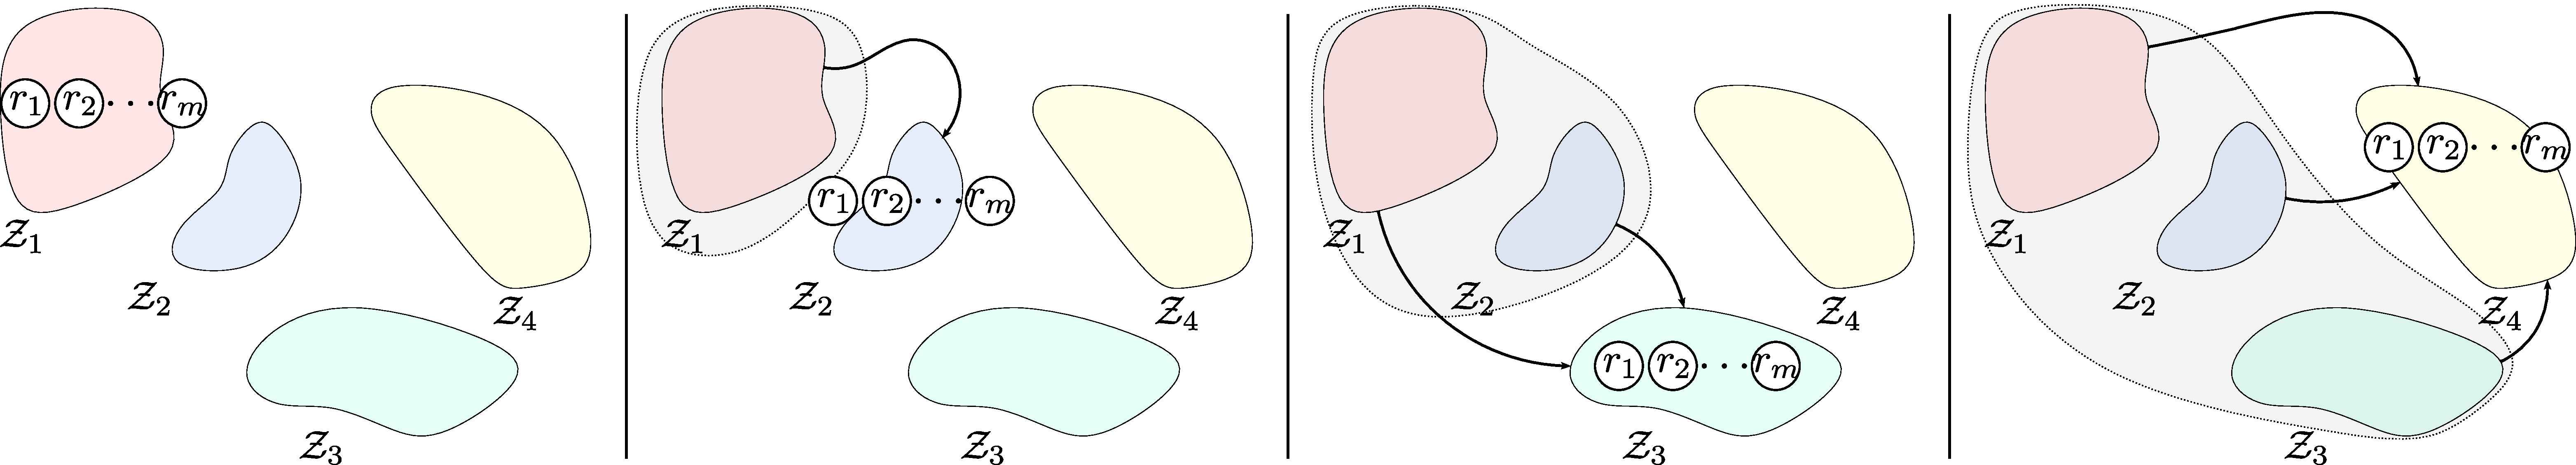
\includegraphics[width= 0.7\textwidth]{fig/cluster_learning_sequence.png} \label{fig:cluster_learning_sequence}}
	\hspace*{\fill}
	\\	
	\hspace*{\fill}
	\subfloat[]{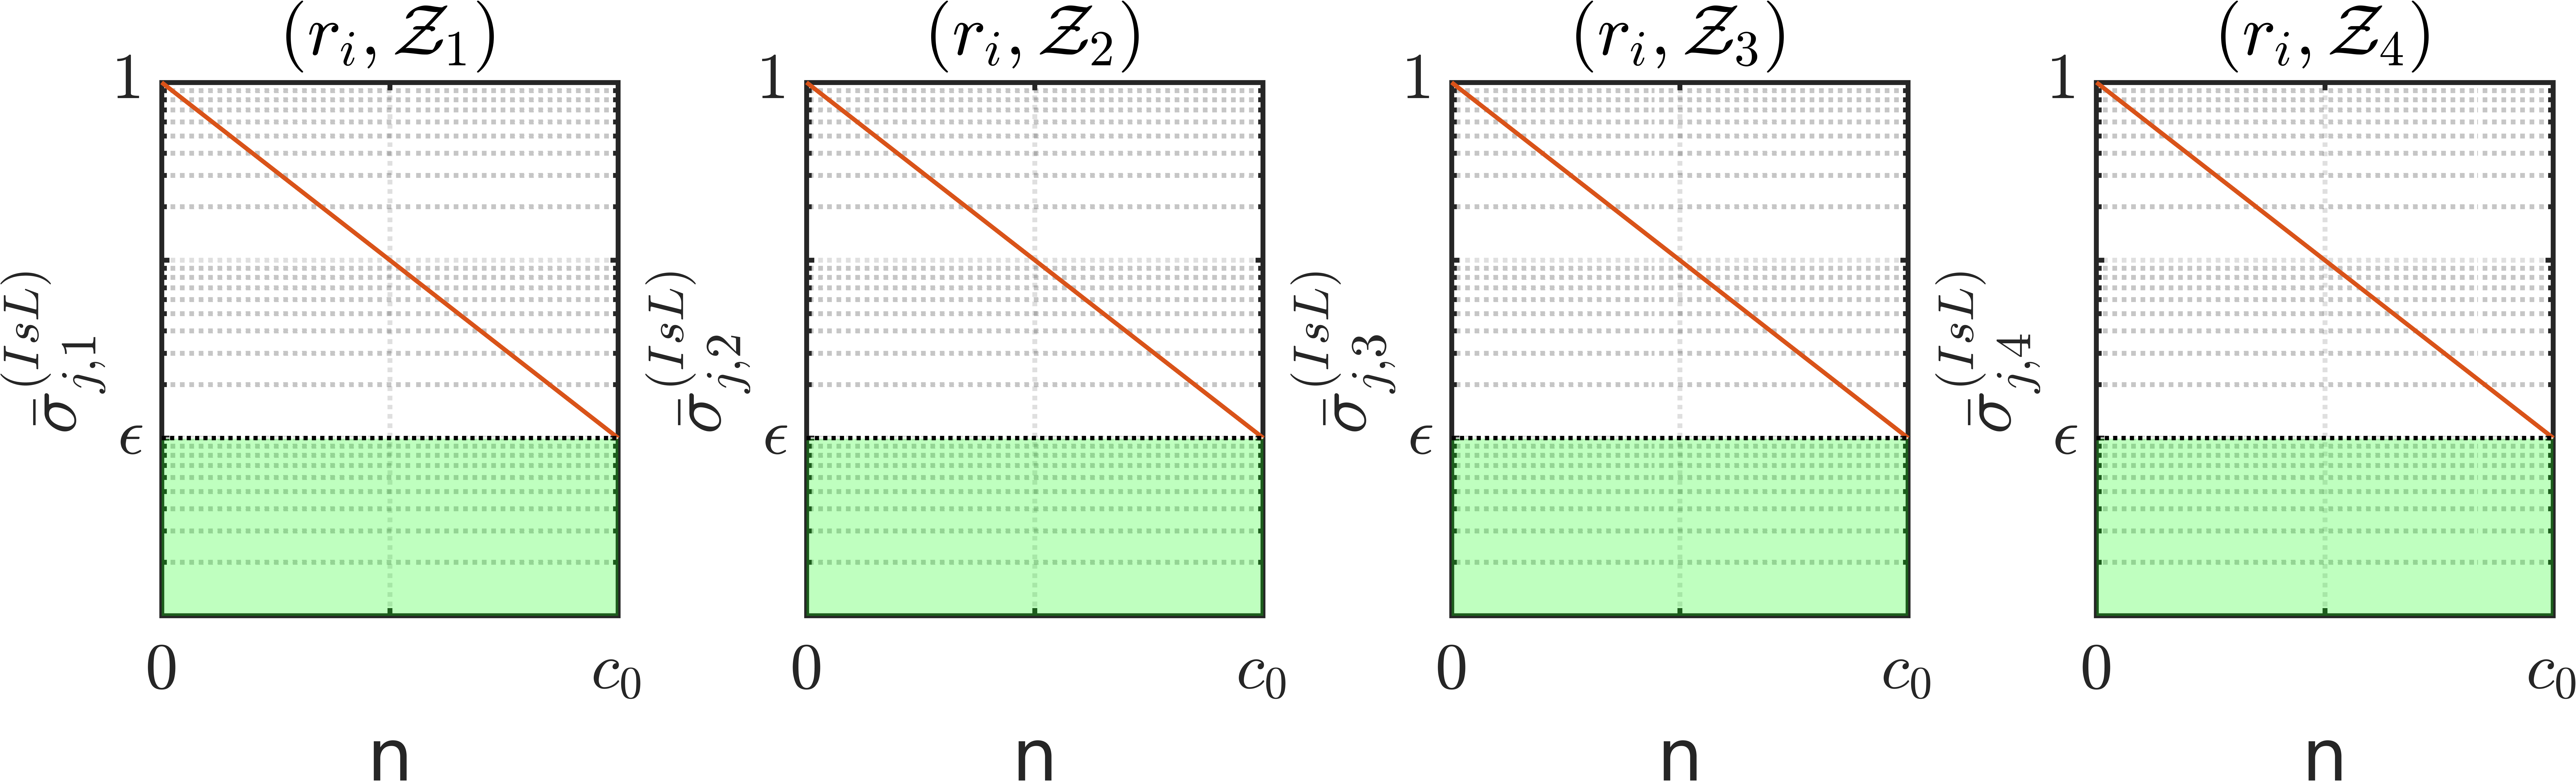
\includegraphics[width= 0.7\textwidth]{fig/dynamics_isolated_learning.png} \label{fig:dynamics_isolated_learning}}  
	\hspace*{\fill}
	\\	
	\hspace*{\fill}
	\subfloat[]{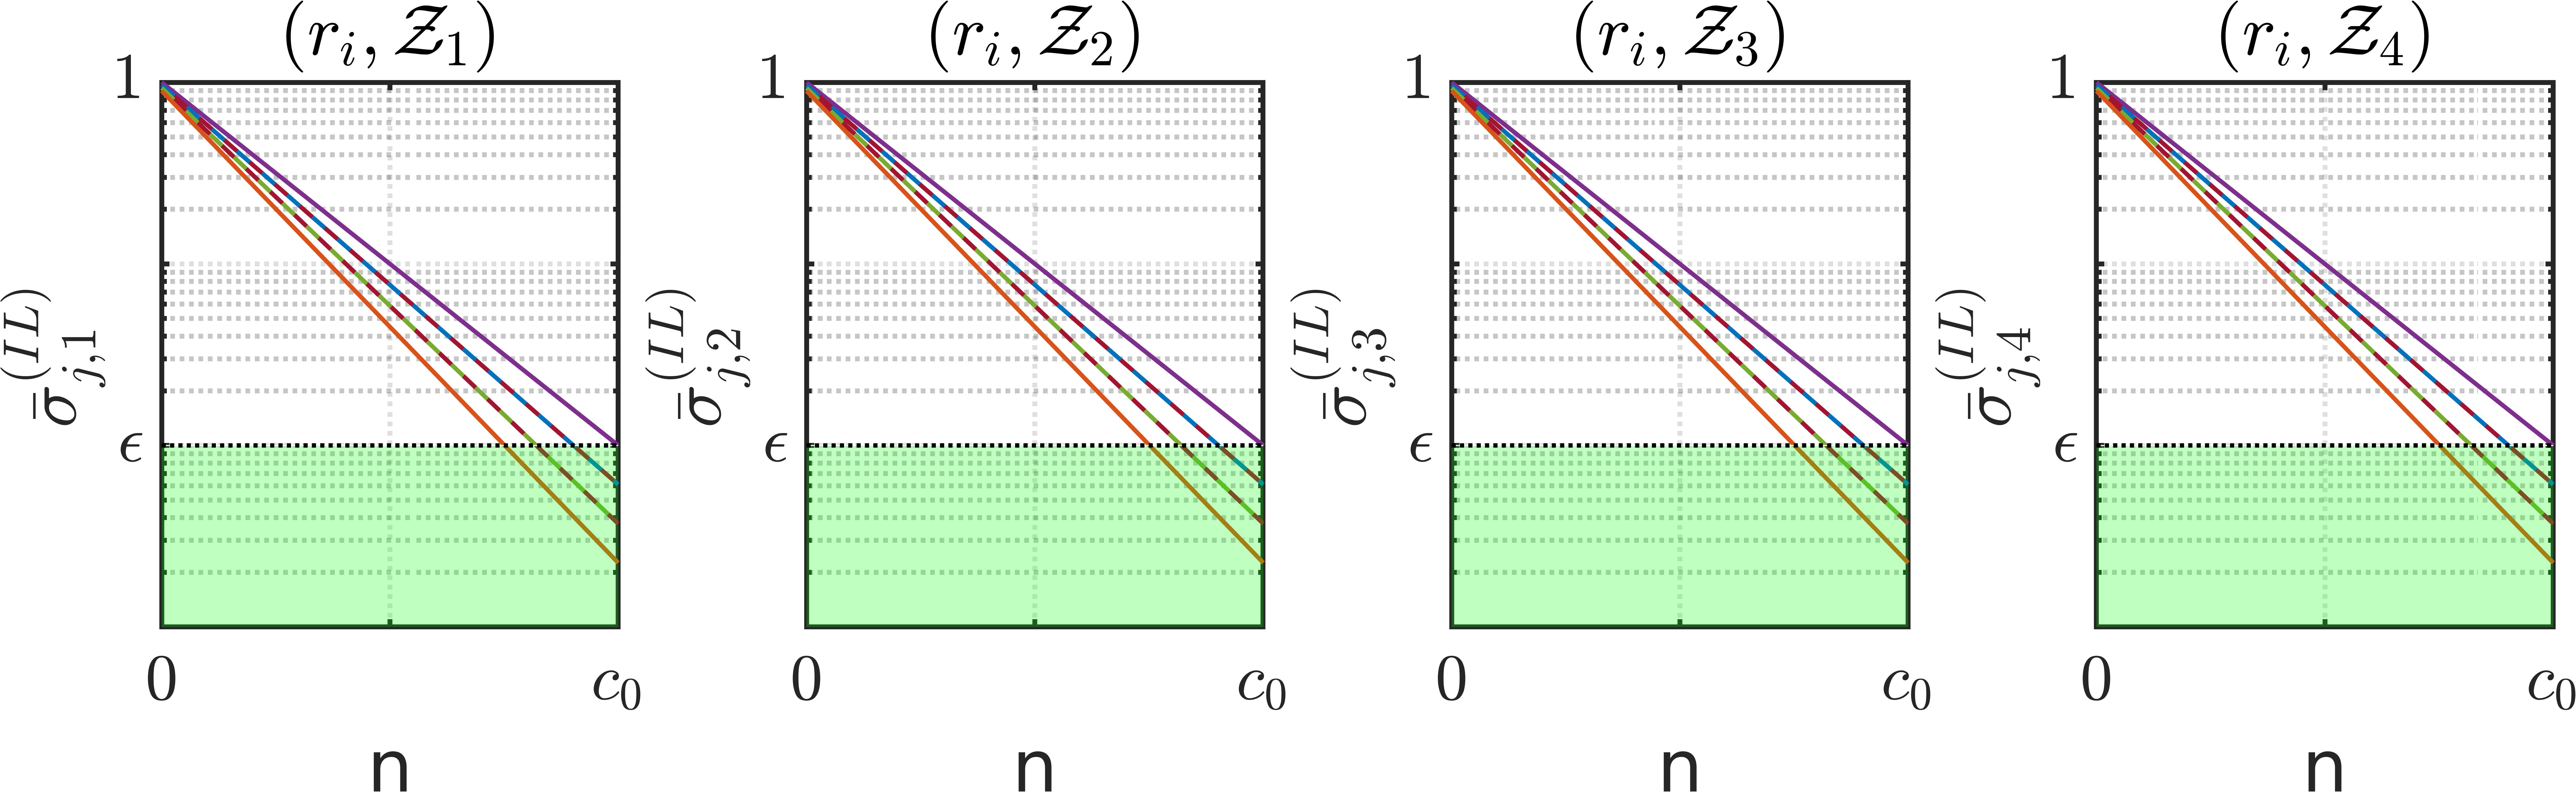
\includegraphics[width= 0.7\textwidth]{fig/dynamics_incremental_learning.png} \label{fig:dynamics_incremental_learning}}  
	\hspace*{\fill}	
	\\
	\hspace*{\fill}
	\subfloat[]{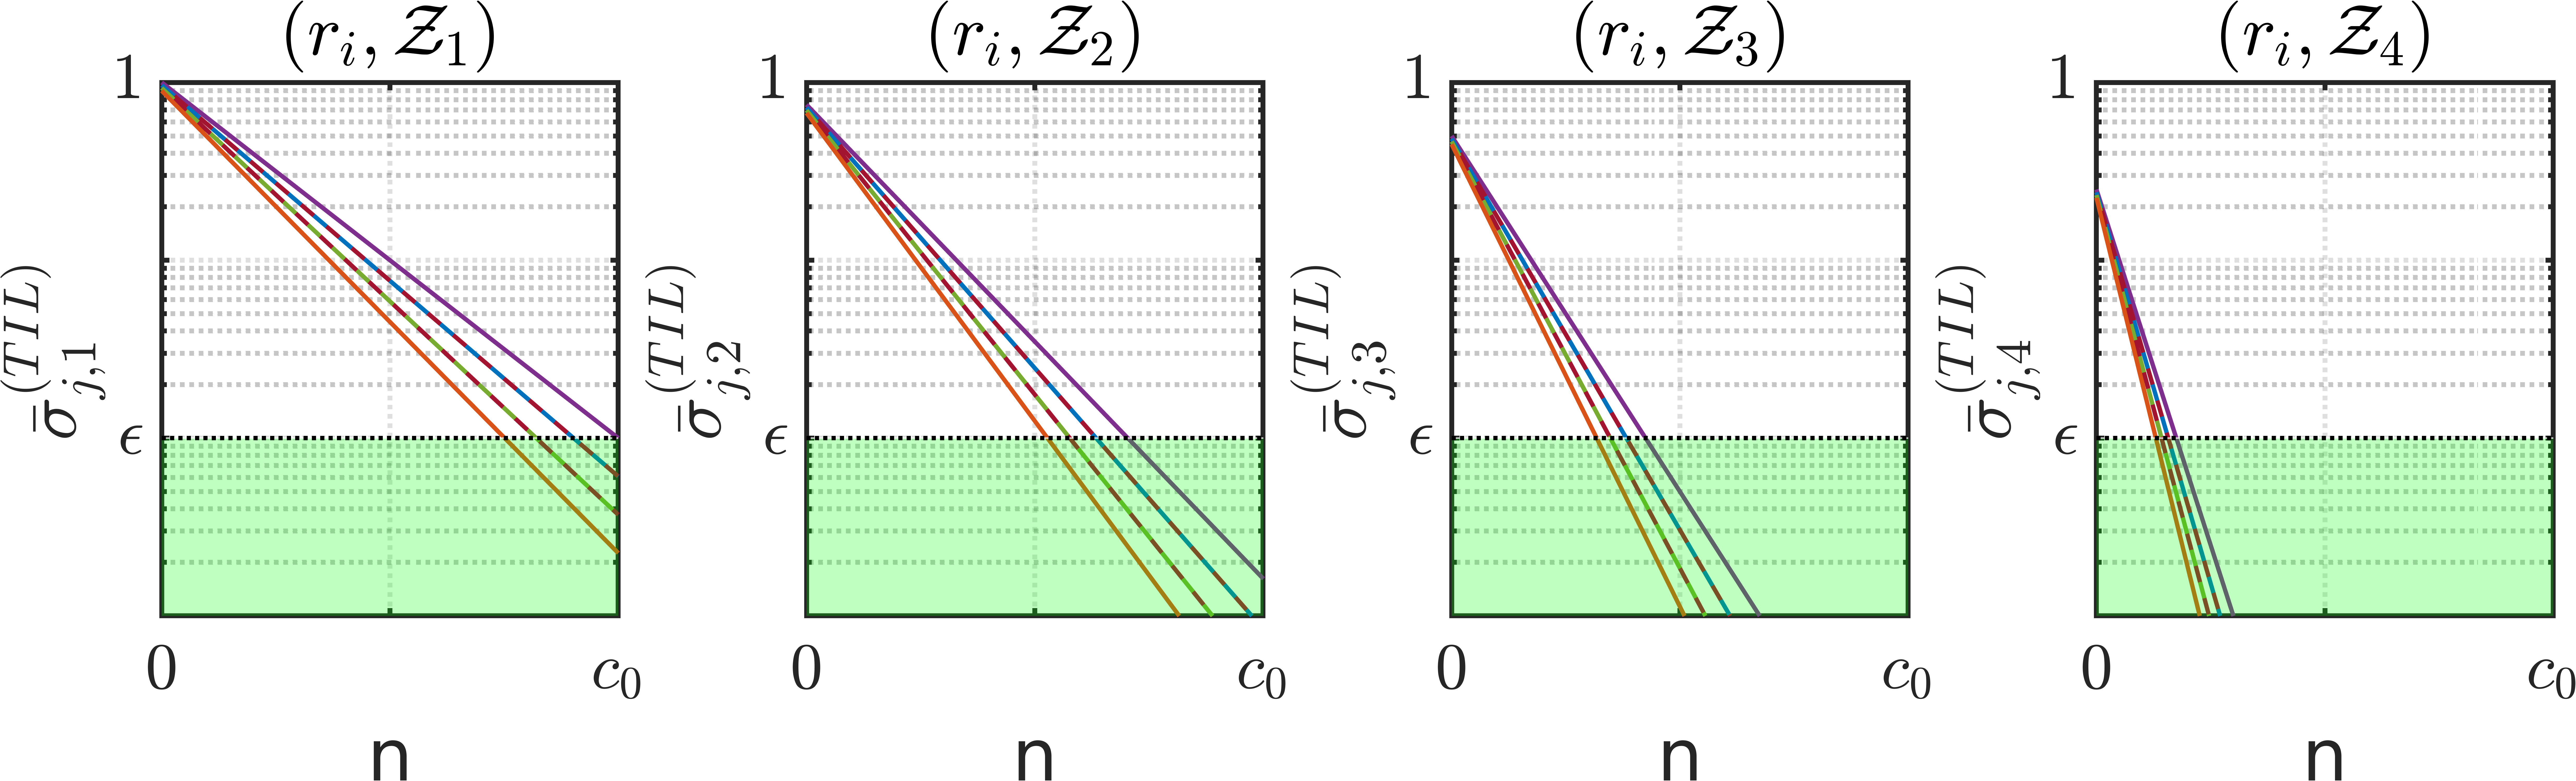
\includegraphics[width= 0.7\textwidth]{fig/dynamics_incremental_transfer_learning.png} \label{fig:dynamics_incremental_transfer_learning}}  
	\hspace*{\fill}
	\\
	\hspace*{\fill}
	\subfloat[]{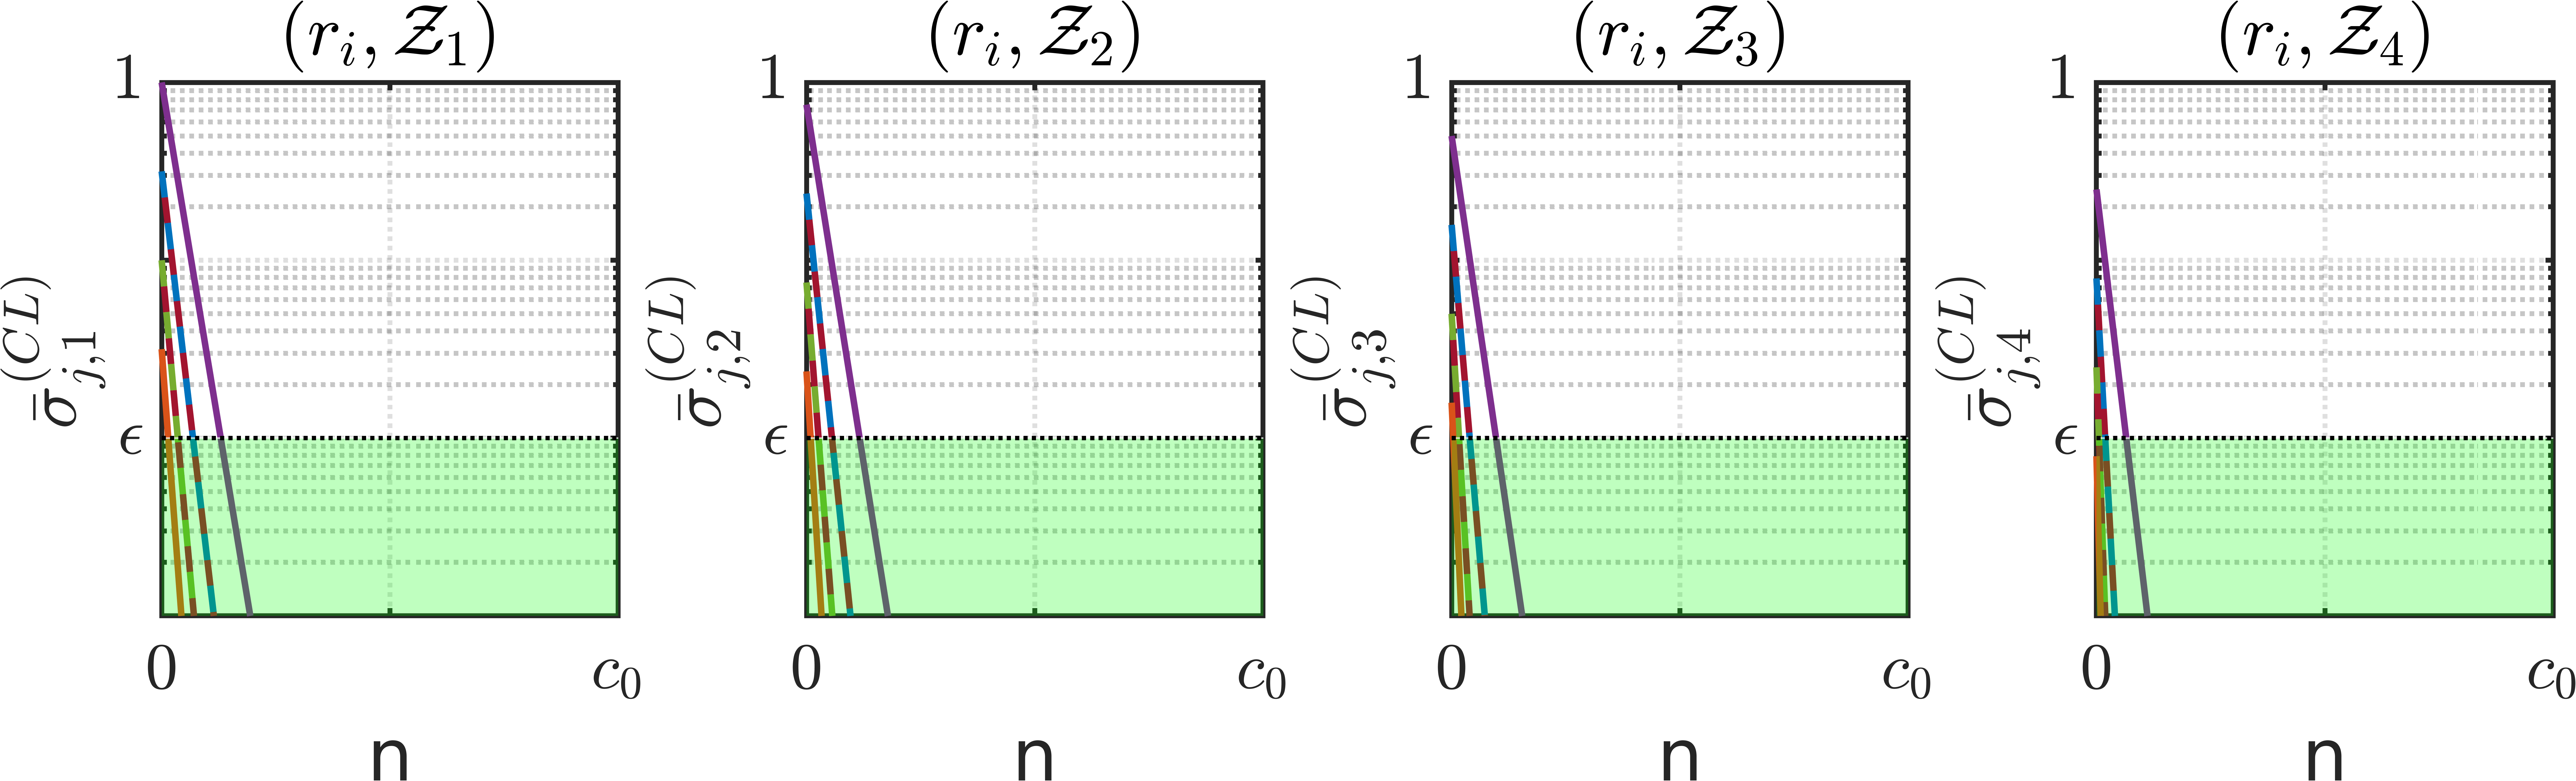
\includegraphics[width= 0.7\textwidth]{fig/dynamics_collective_learning.png} \label{fig:dynamics_collective_learning}}
	\hspace*{\fill}
	\caption[] {\label{fig:collective_learning} Scenario 1: \subref{fig:cluster_learning_sequence} the skills of each cluster are learned by the $ m$ robots in succession, \subref{fig:dynamics_isolated_learning} isolated learning, \subref{fig:dynamics_incremental_learning} incremental learning,  \subref{fig:dynamics_incremental_transfer_learning} incremental + transfer learning, \subref{fig:dynamics_collective_learning} collective learning.}
\end{figure}
% ---


% ===================================================================================================
%                                                 |                                                 |
%                                                 |                                                 |
% -------------------------------------------- SECTION ---------------------------------------------|
%                                                 |                                                 |
%                                                 |                                                 |
% ===================================================================================================
\newpage
\section{Supporting statistics}
% ===================================================================================================
\subsection{Industrial and cobot statistics}\label{sec:robot_statistics}
According to the International Federation of Robotics (IFR) the unit sales of collaborative robots in relation to conventional industrial robots has been constantly increasing in the past years \cite{statista_ir_cobot_share}. Recent data, see Fig.~\ref{fig:industrial_cobot_share}, shows that cobots now make almost 15 \% of the sales.
%---
\begin{figure}[!h]
	\centering
	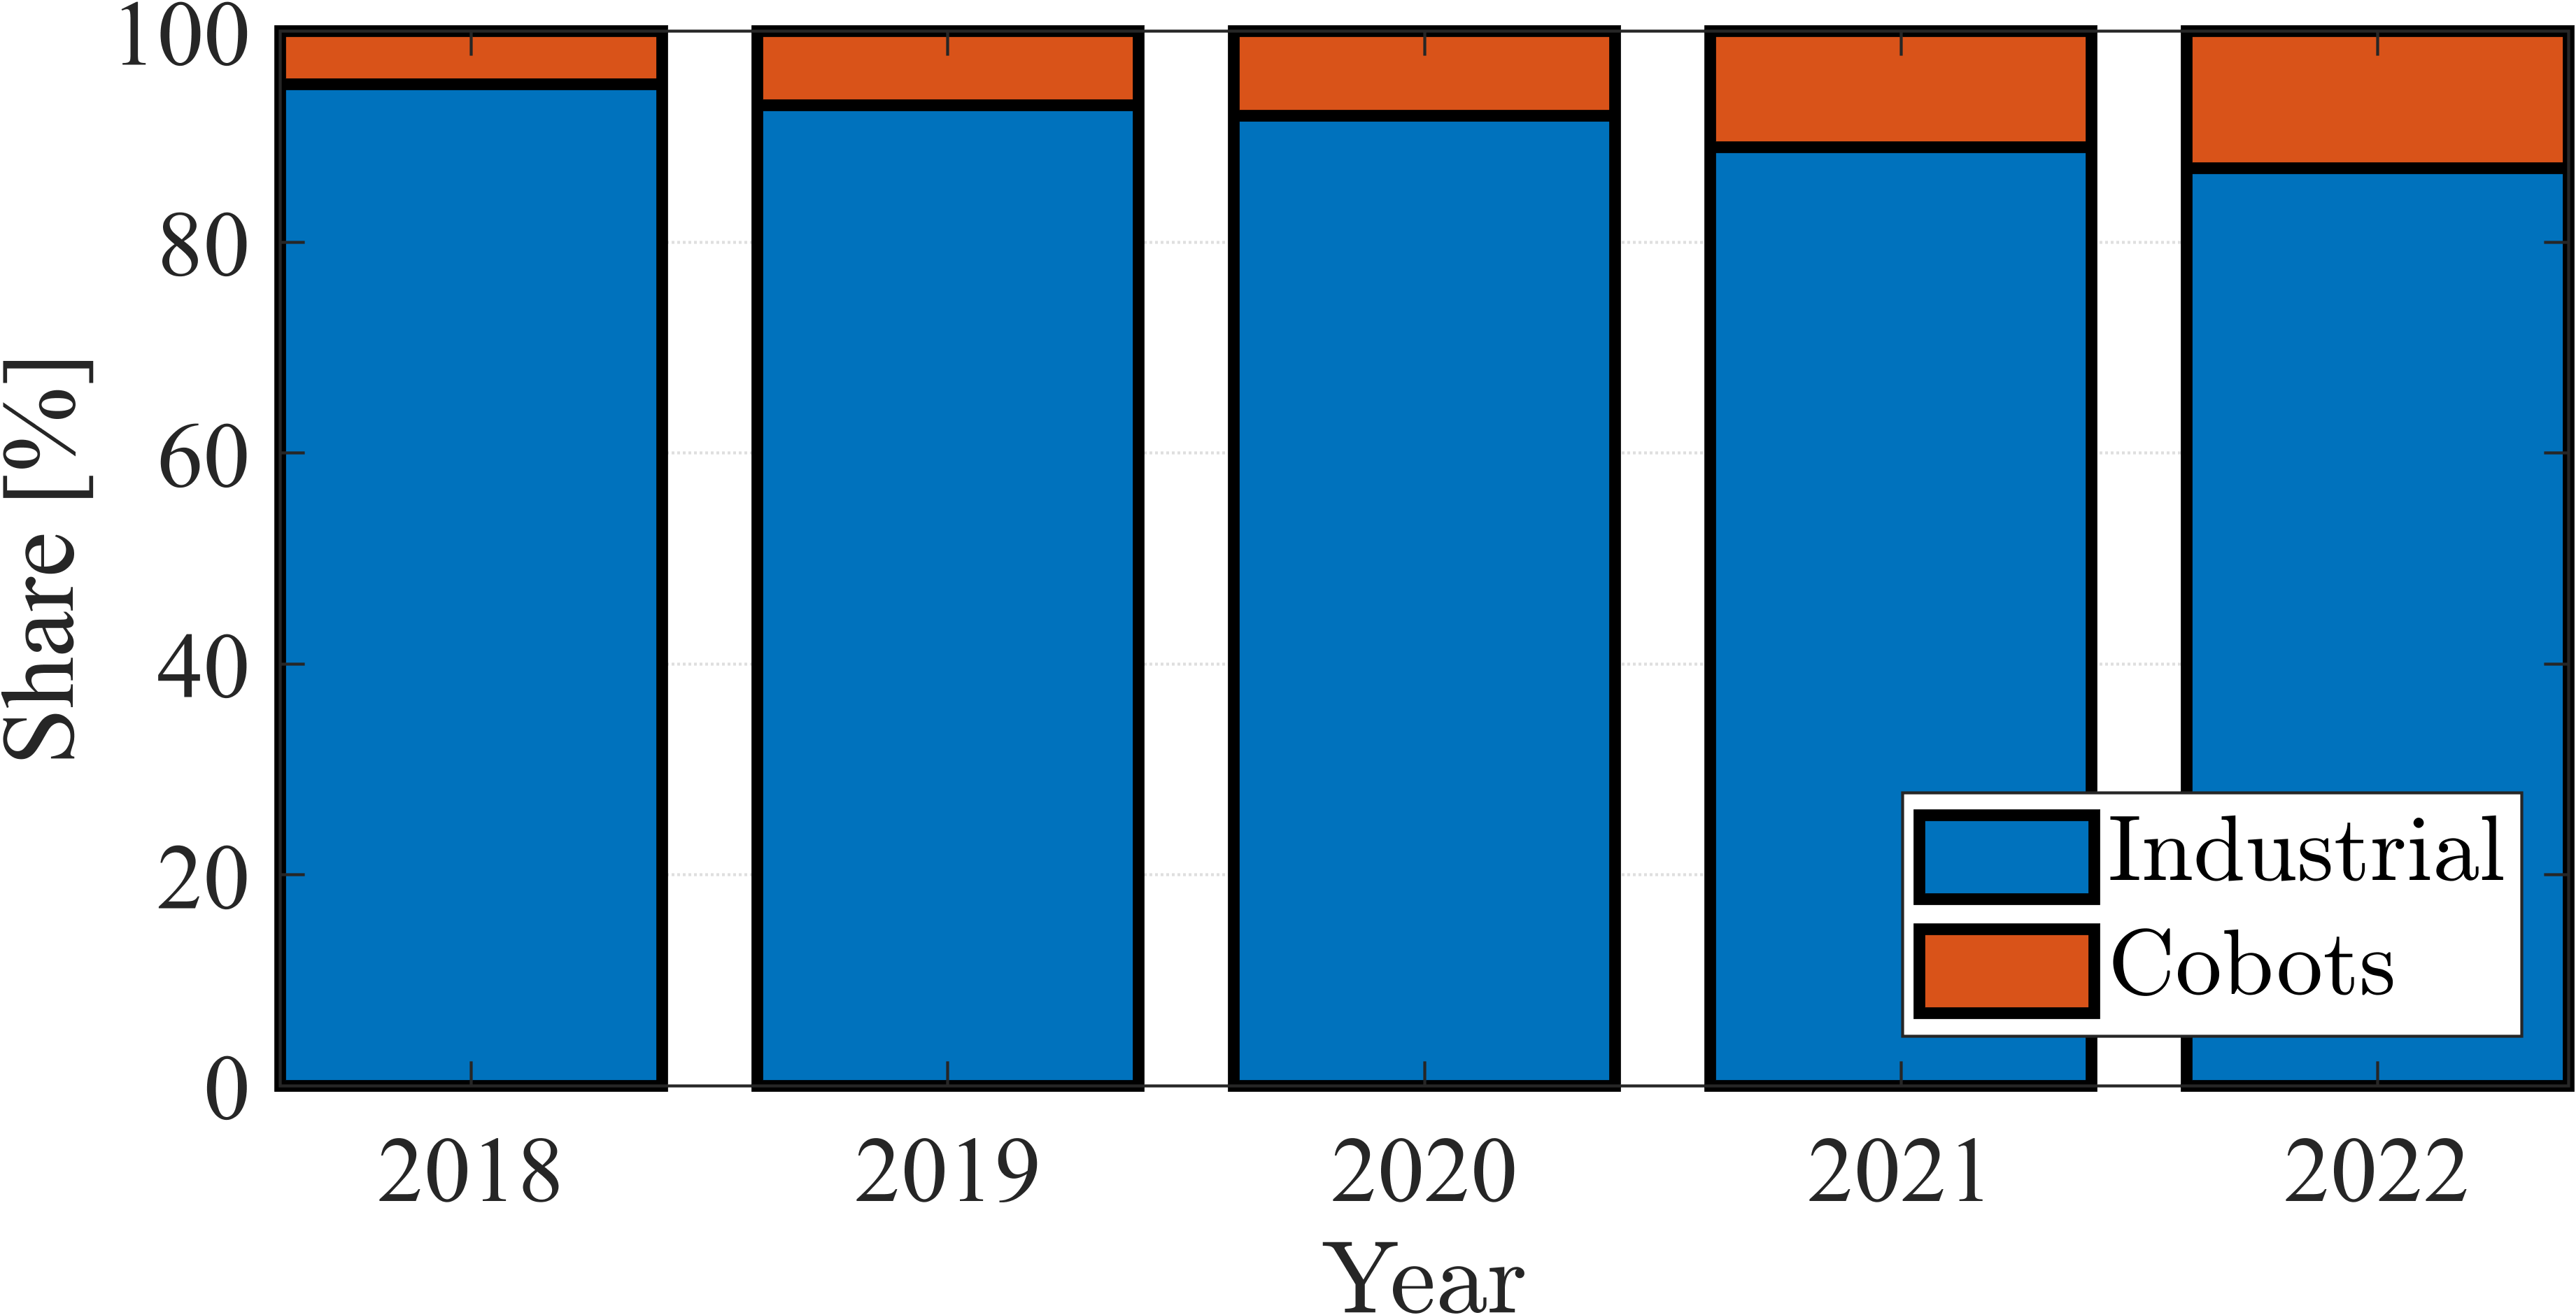
\includegraphics[width= 0.45\textwidth]{fig/share_industrial_and_cobots.png} 
	\caption{Unit sales share industrial robots to cobots }
	\label{fig:industrial_cobot_share}
\end{figure}
% ---

The unit sales are congruent with the the estimated operational stock of industrial (Fig.~\ref{fig:ir_stock}) robots and cobots (\ref{fig:cobot_stock}).
% ---
\begin{figure*}[!h]
	\centering
	\hspace*{\fill}
	\begin{subfigure}[t]{0.45\textwidth}
		\subcaption{}
		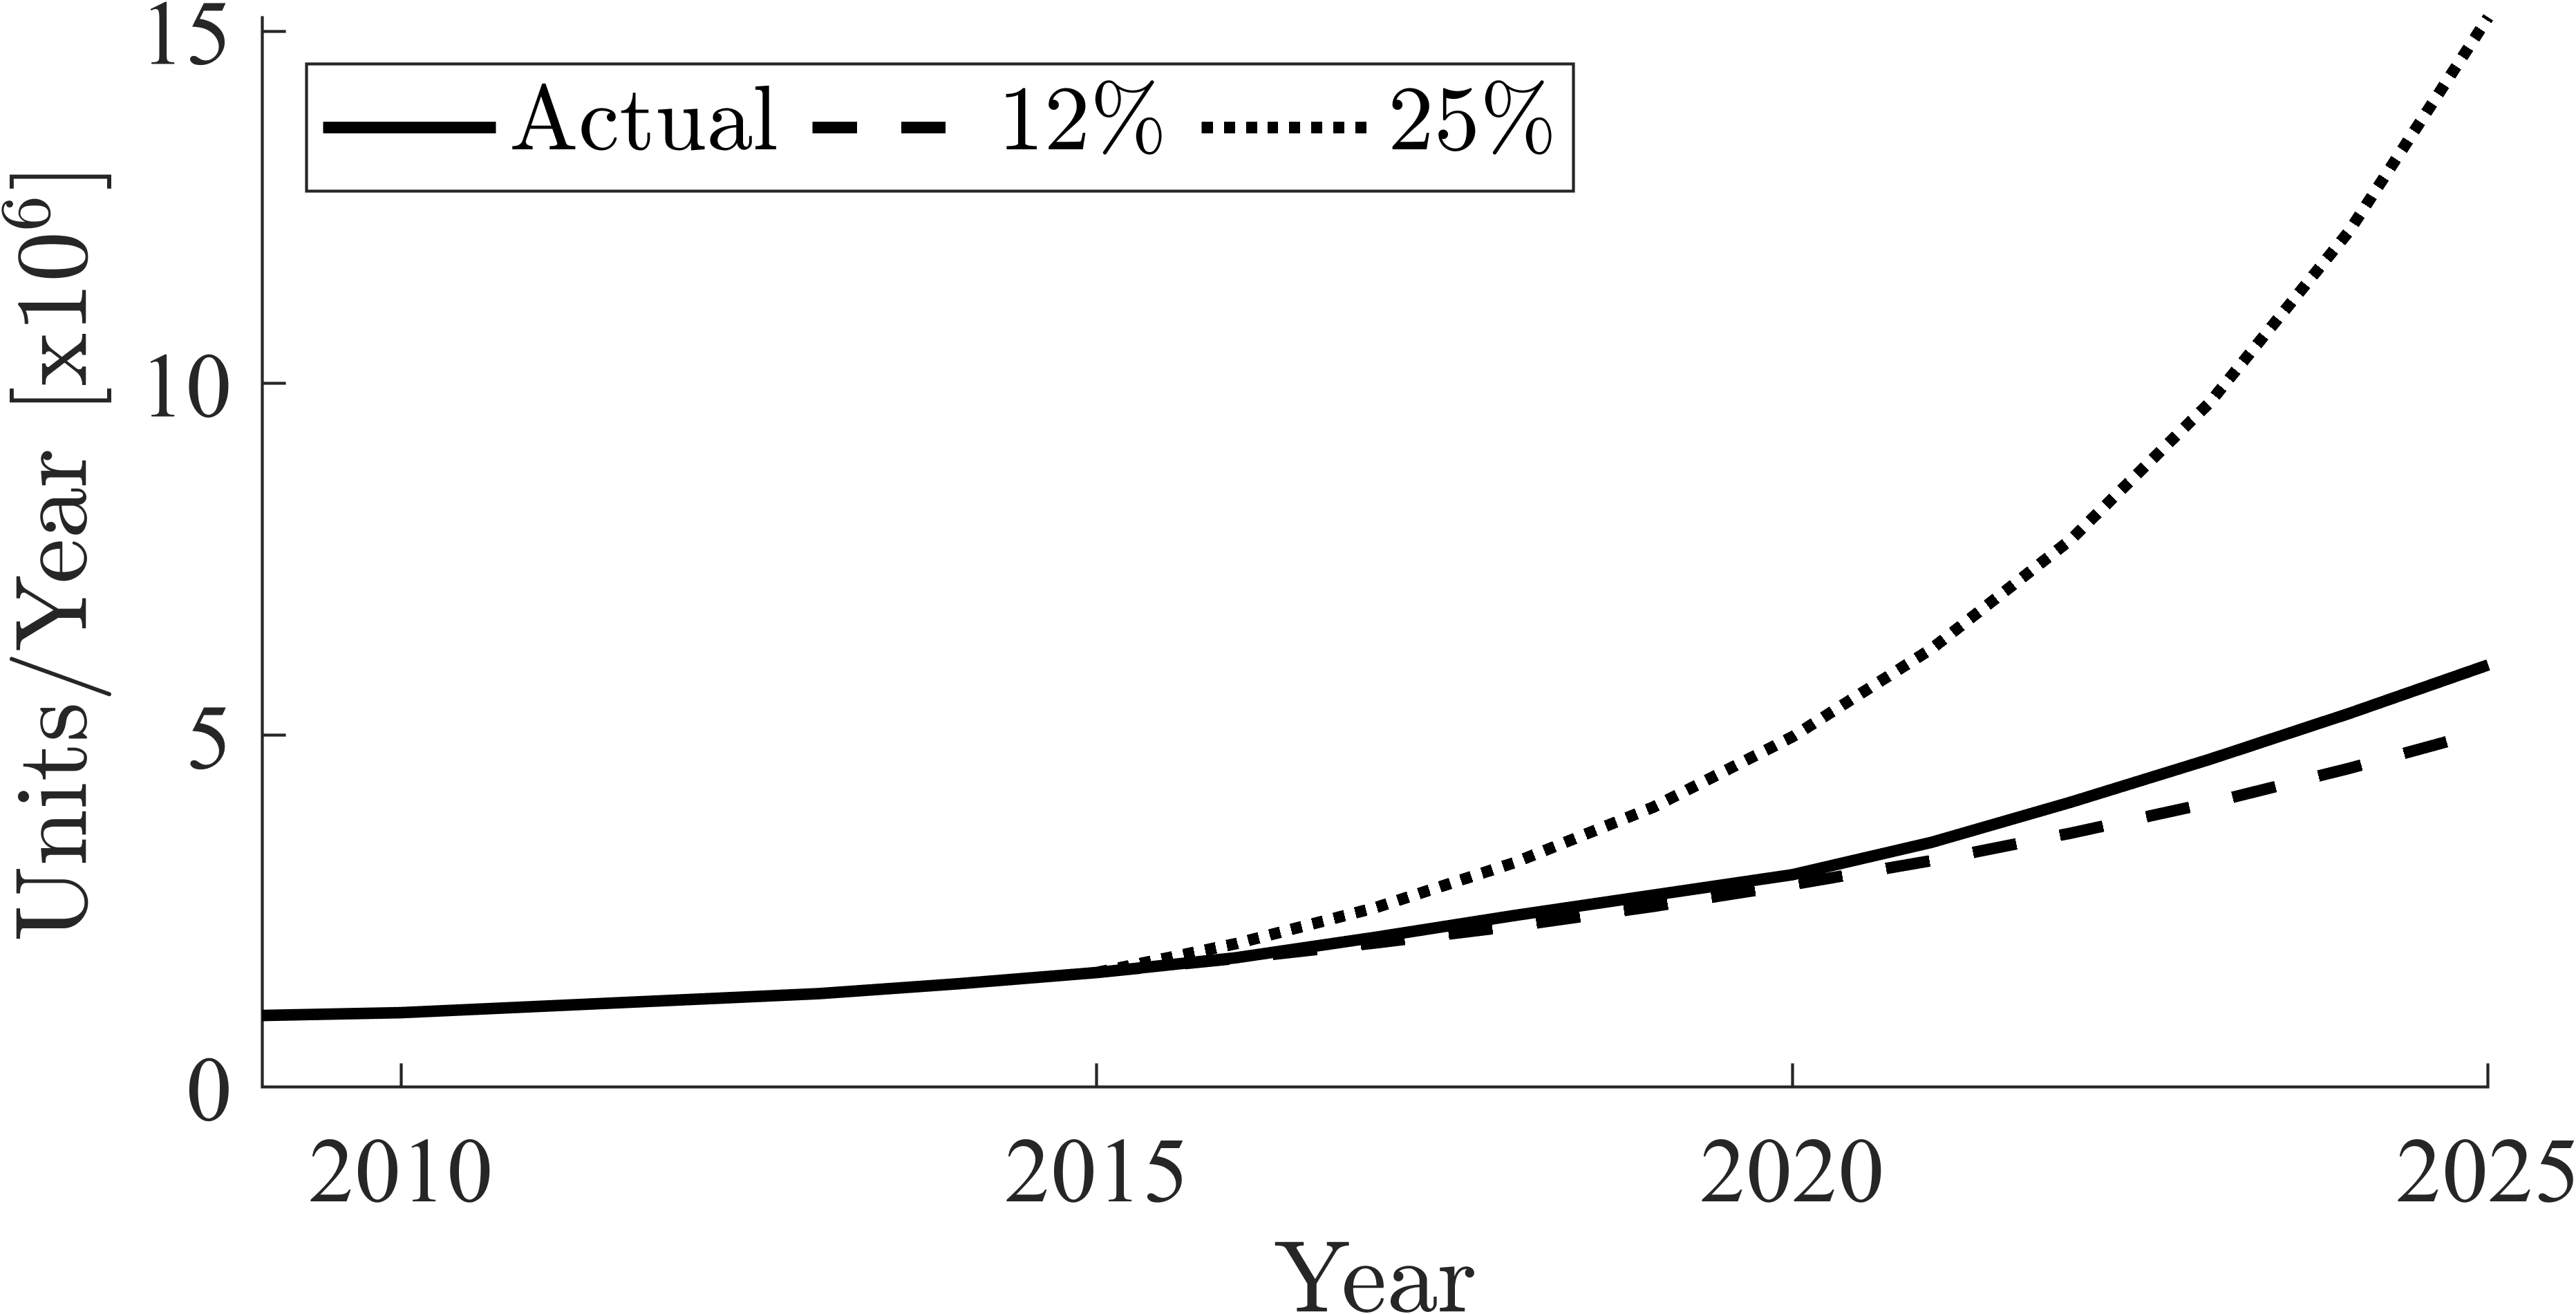
\includegraphics[width= \textwidth]{ir_units_projections.png}
		\label{fig:ir_stock}
	\end{subfigure}
	\hfill
	\begin{subfigure}[t]{0.45\textwidth}
		\subcaption{}
		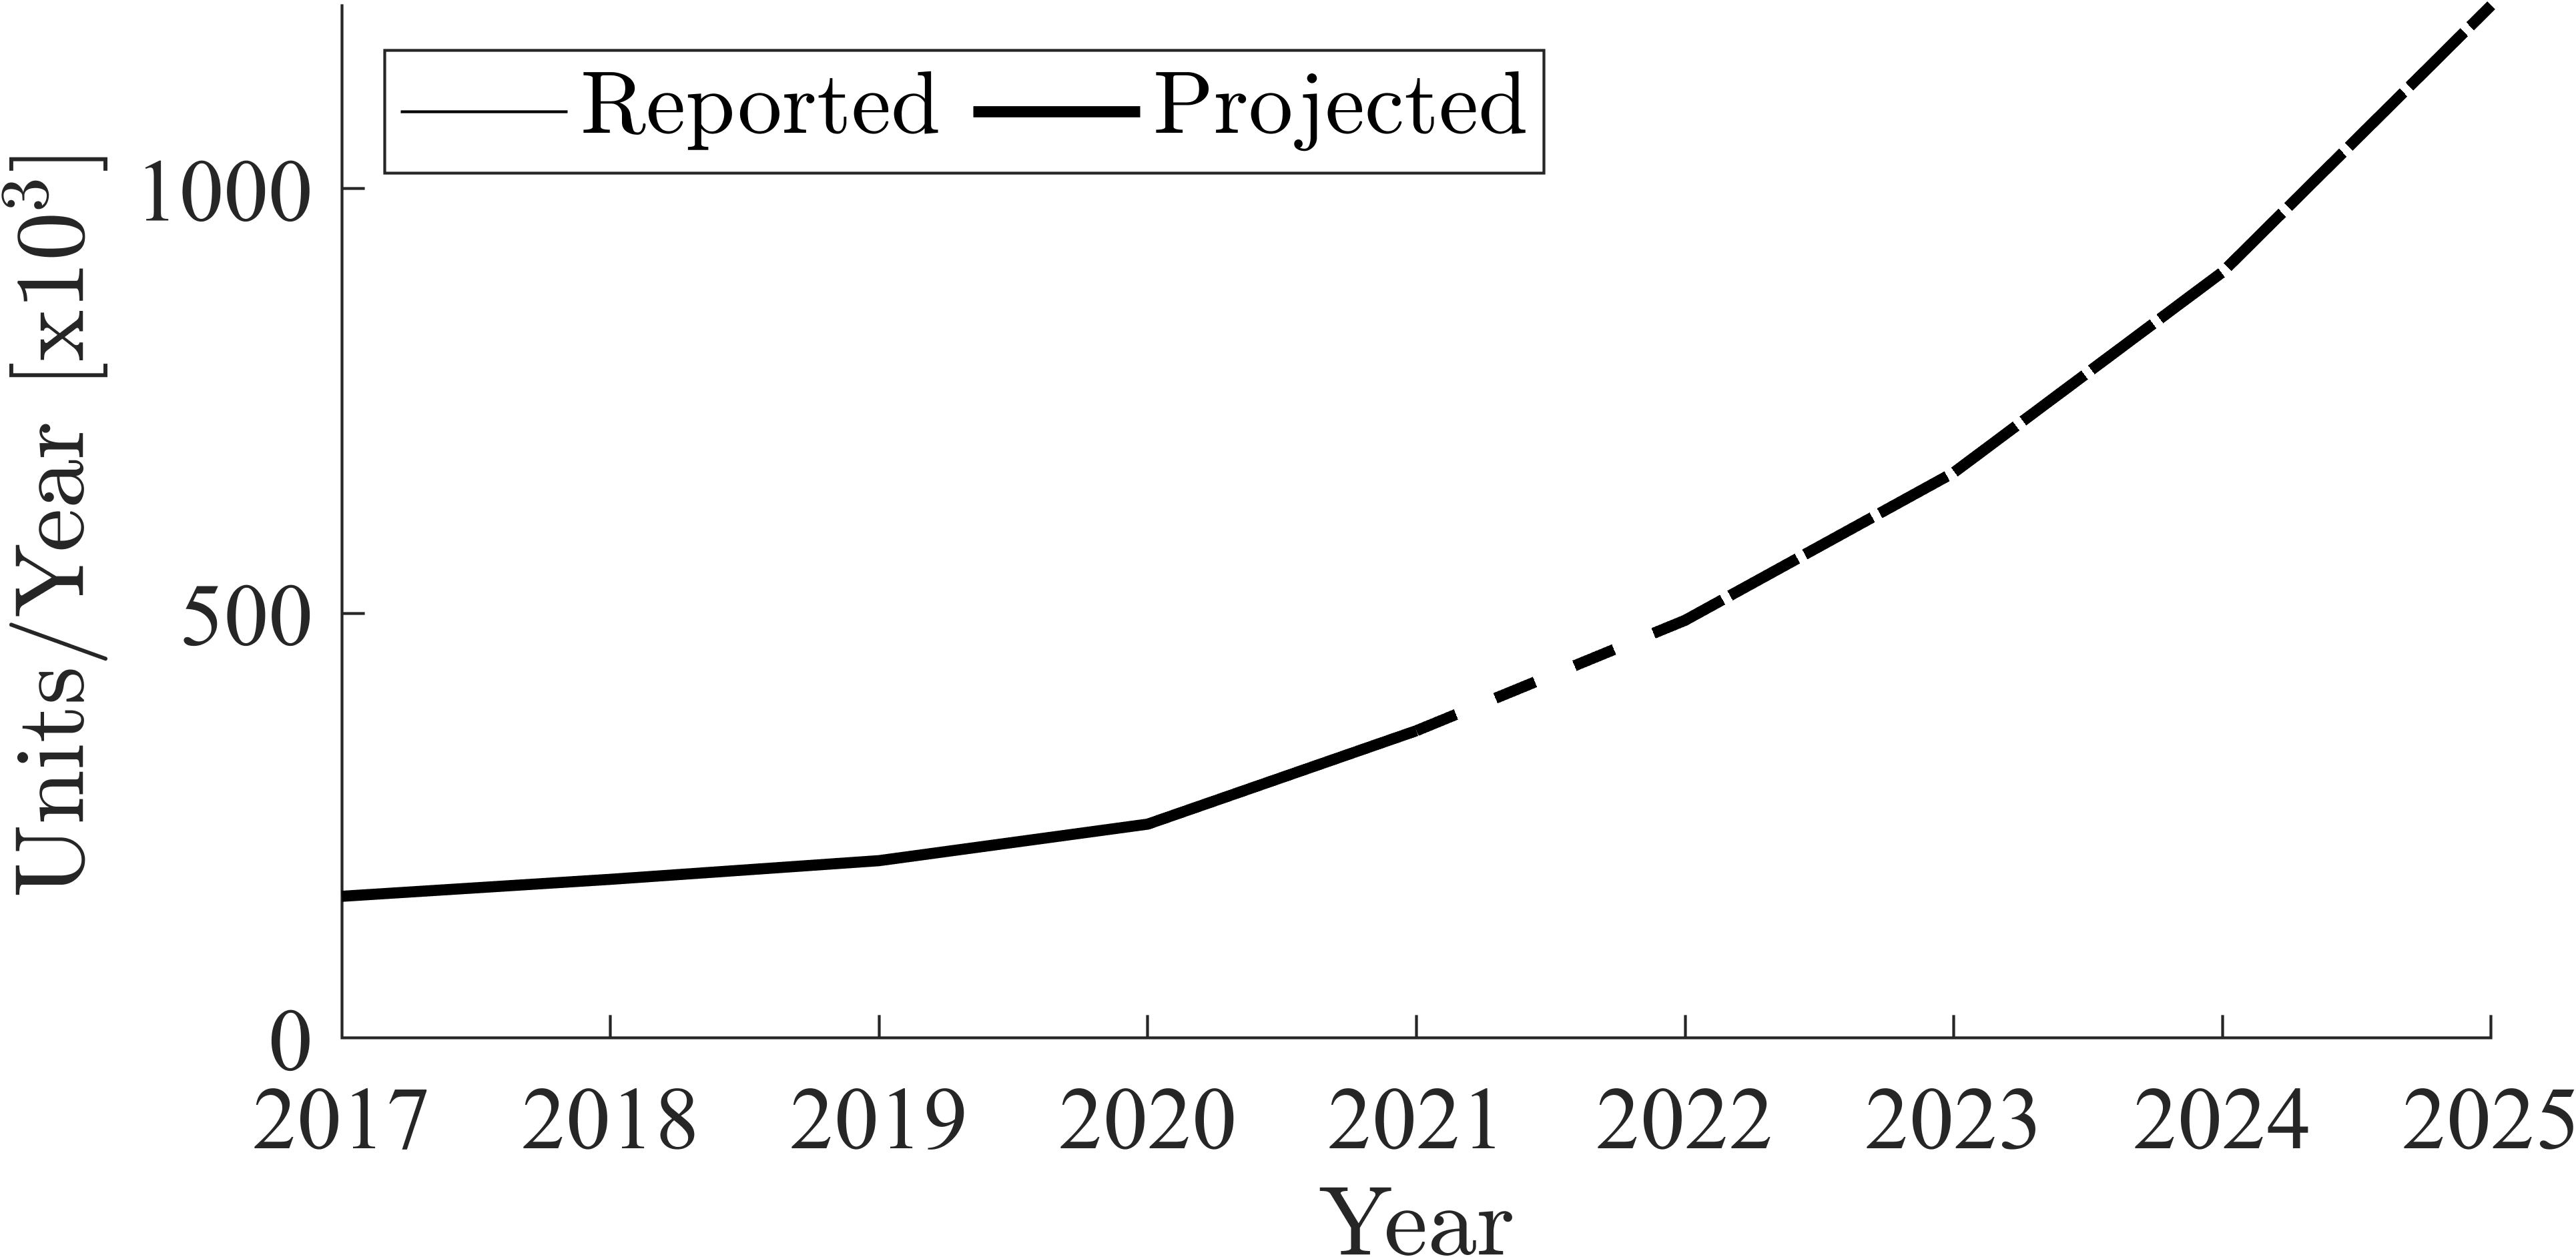
\includegraphics[width= \textwidth]{cb_units_projections.png}
		\label{fig:cobot_stock}
	\end{subfigure}
	\hspace*{\fill}	
	\caption[] {\label{fig:robot_forecasts} Forecasts for robot operational stock. \subref{fig:ir_stock} industrial robots install base forecast and \subref{fig:cobot_stock} cobots install base forecast.}	
\end{figure*}
% ===================================================================================================
%                                                 |                                                 |
%                                                 |                                                 |
% -------------------------------------------- SECTION ---------------------------------------------|
%                                                 |                                                 |
%                                                 |                                                 |
% ===================================================================================================
\newpage
\section{Industrial robot energy consumption support data}\label{sec:app_robot_ener_consumption}
To provide estimates of the worldwide energy consumption of industrial and collaborative robots we surveyed various sources including reports from consulting agencies and non-profit organizations, news articles and manufacturer press releases and data-sheets to determine essential data such as the operational stock and power consumption per type of robot.

\subsection{Industrial robots}
According to \cite{montaqim2015} and available press releases of different robotic companies \cite{fanuc2015, yaskawa2014, ABB2015}, the approximate distribution of the industrial robot install base per manufacturer is shown in Fig.~\ref{fig:manufacturers_pie}.
% ---
\begin{figure*}[!h]
	\centering
	\hspace*{\fill}
	\begin{subfigure}[t]{0.45\textwidth}
		\subcaption{}
		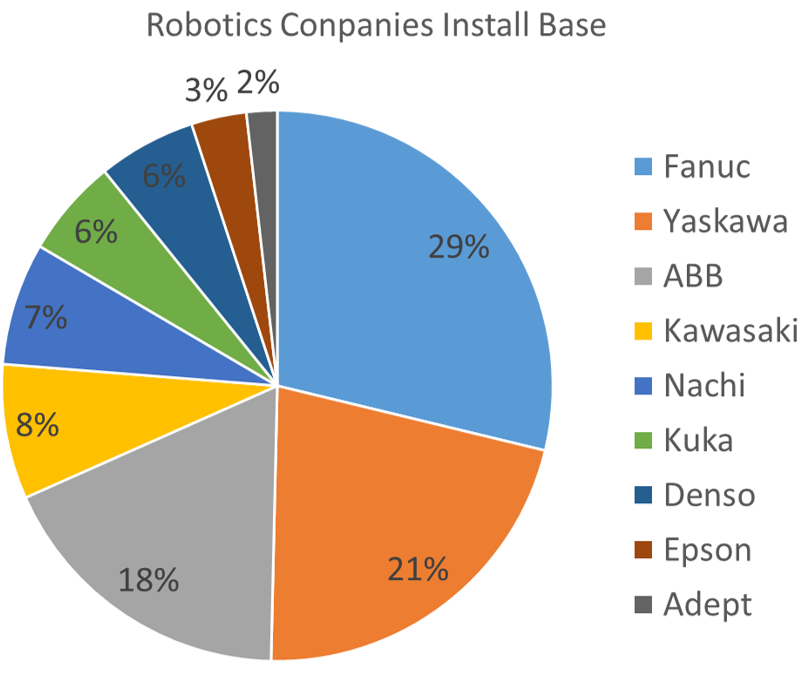
\includegraphics[width= \textwidth]{manufacturers}
		\label{fig:manufacturers_pie}
	\end{subfigure}
	\hfill
	\begin{subfigure}[t]{0.45\textwidth}
		\subcaption{}
		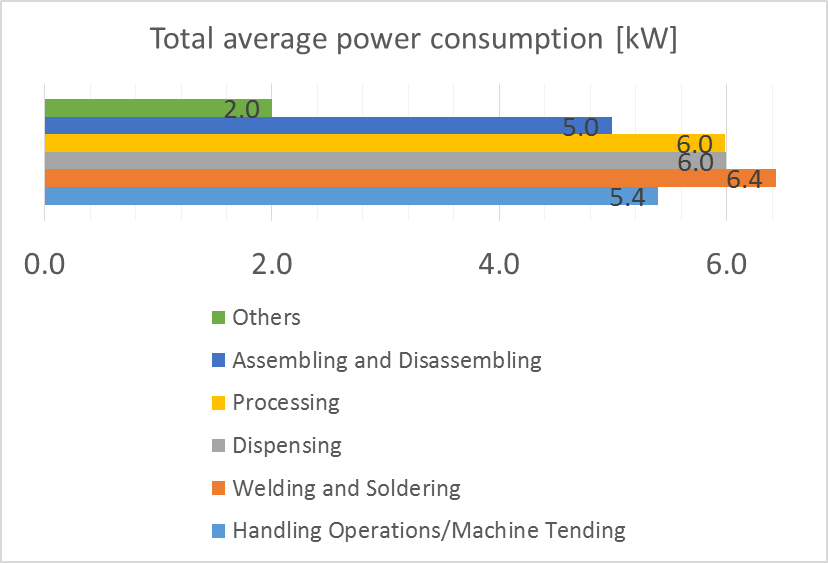
\includegraphics[width=\textwidth]{industrial_robots_average_power_per_category} \label{fig:ir_average_power}
	\end{subfigure}
	\hspace*{\fill}
	\caption[] {\label{fig:ir_statistics} Industrial robots statistics. \subref{fig:manufacturers_pie} Percentage of installed industrial robots per manufacturer and \subref{fig:ir_average_power} average power consumption of industrial robots per category.}
\end{figure*}
% ---

Since Fanuc, Yaskawa, and ABB make for two-thirds of the total install base of industrial robots, we took the power consumption of the robots from those manufacturers to estimate the total power consumption. After surveying the data-sheets for the different robot types in their portfolio, the average power consumption for each model was estimated. Additionally, every manufacturer classifies their robots according to one or more possible applications, which can be grouped into the application categories defined by the IFR. The average power consumption was calculated for every application using the values reported in the robot data-sheets. Finally, the power consumption for each category was computed as a weighted average based on the companies' market share percentage (assuming that 68 \% is the total number of robots)\footnote[1]{These numbers should be used with discretion since there is no available information on which are the most common installed robot models. This information may change the estimation.}. The estimated power consumption per robot application is shown in Fig.~\ref{fig:ir_average_power}. Using these numbers and the estimated operational stock of industrial robots reported in \cite{statista_ir_operational_stock} and by the International Federation of Robotics (see Fig.~\ref{fig:ir_stock}), the estimated worldwide industrial robot energy consumption was computed and shown in Fig.~\ref{fig:ir_energy}.

% ===================================================================================================
\subsection{Collaborative robots}\label{sec:app_cobot_ener_consumption}
%---
\begin{figure}[!h]
	\centering
	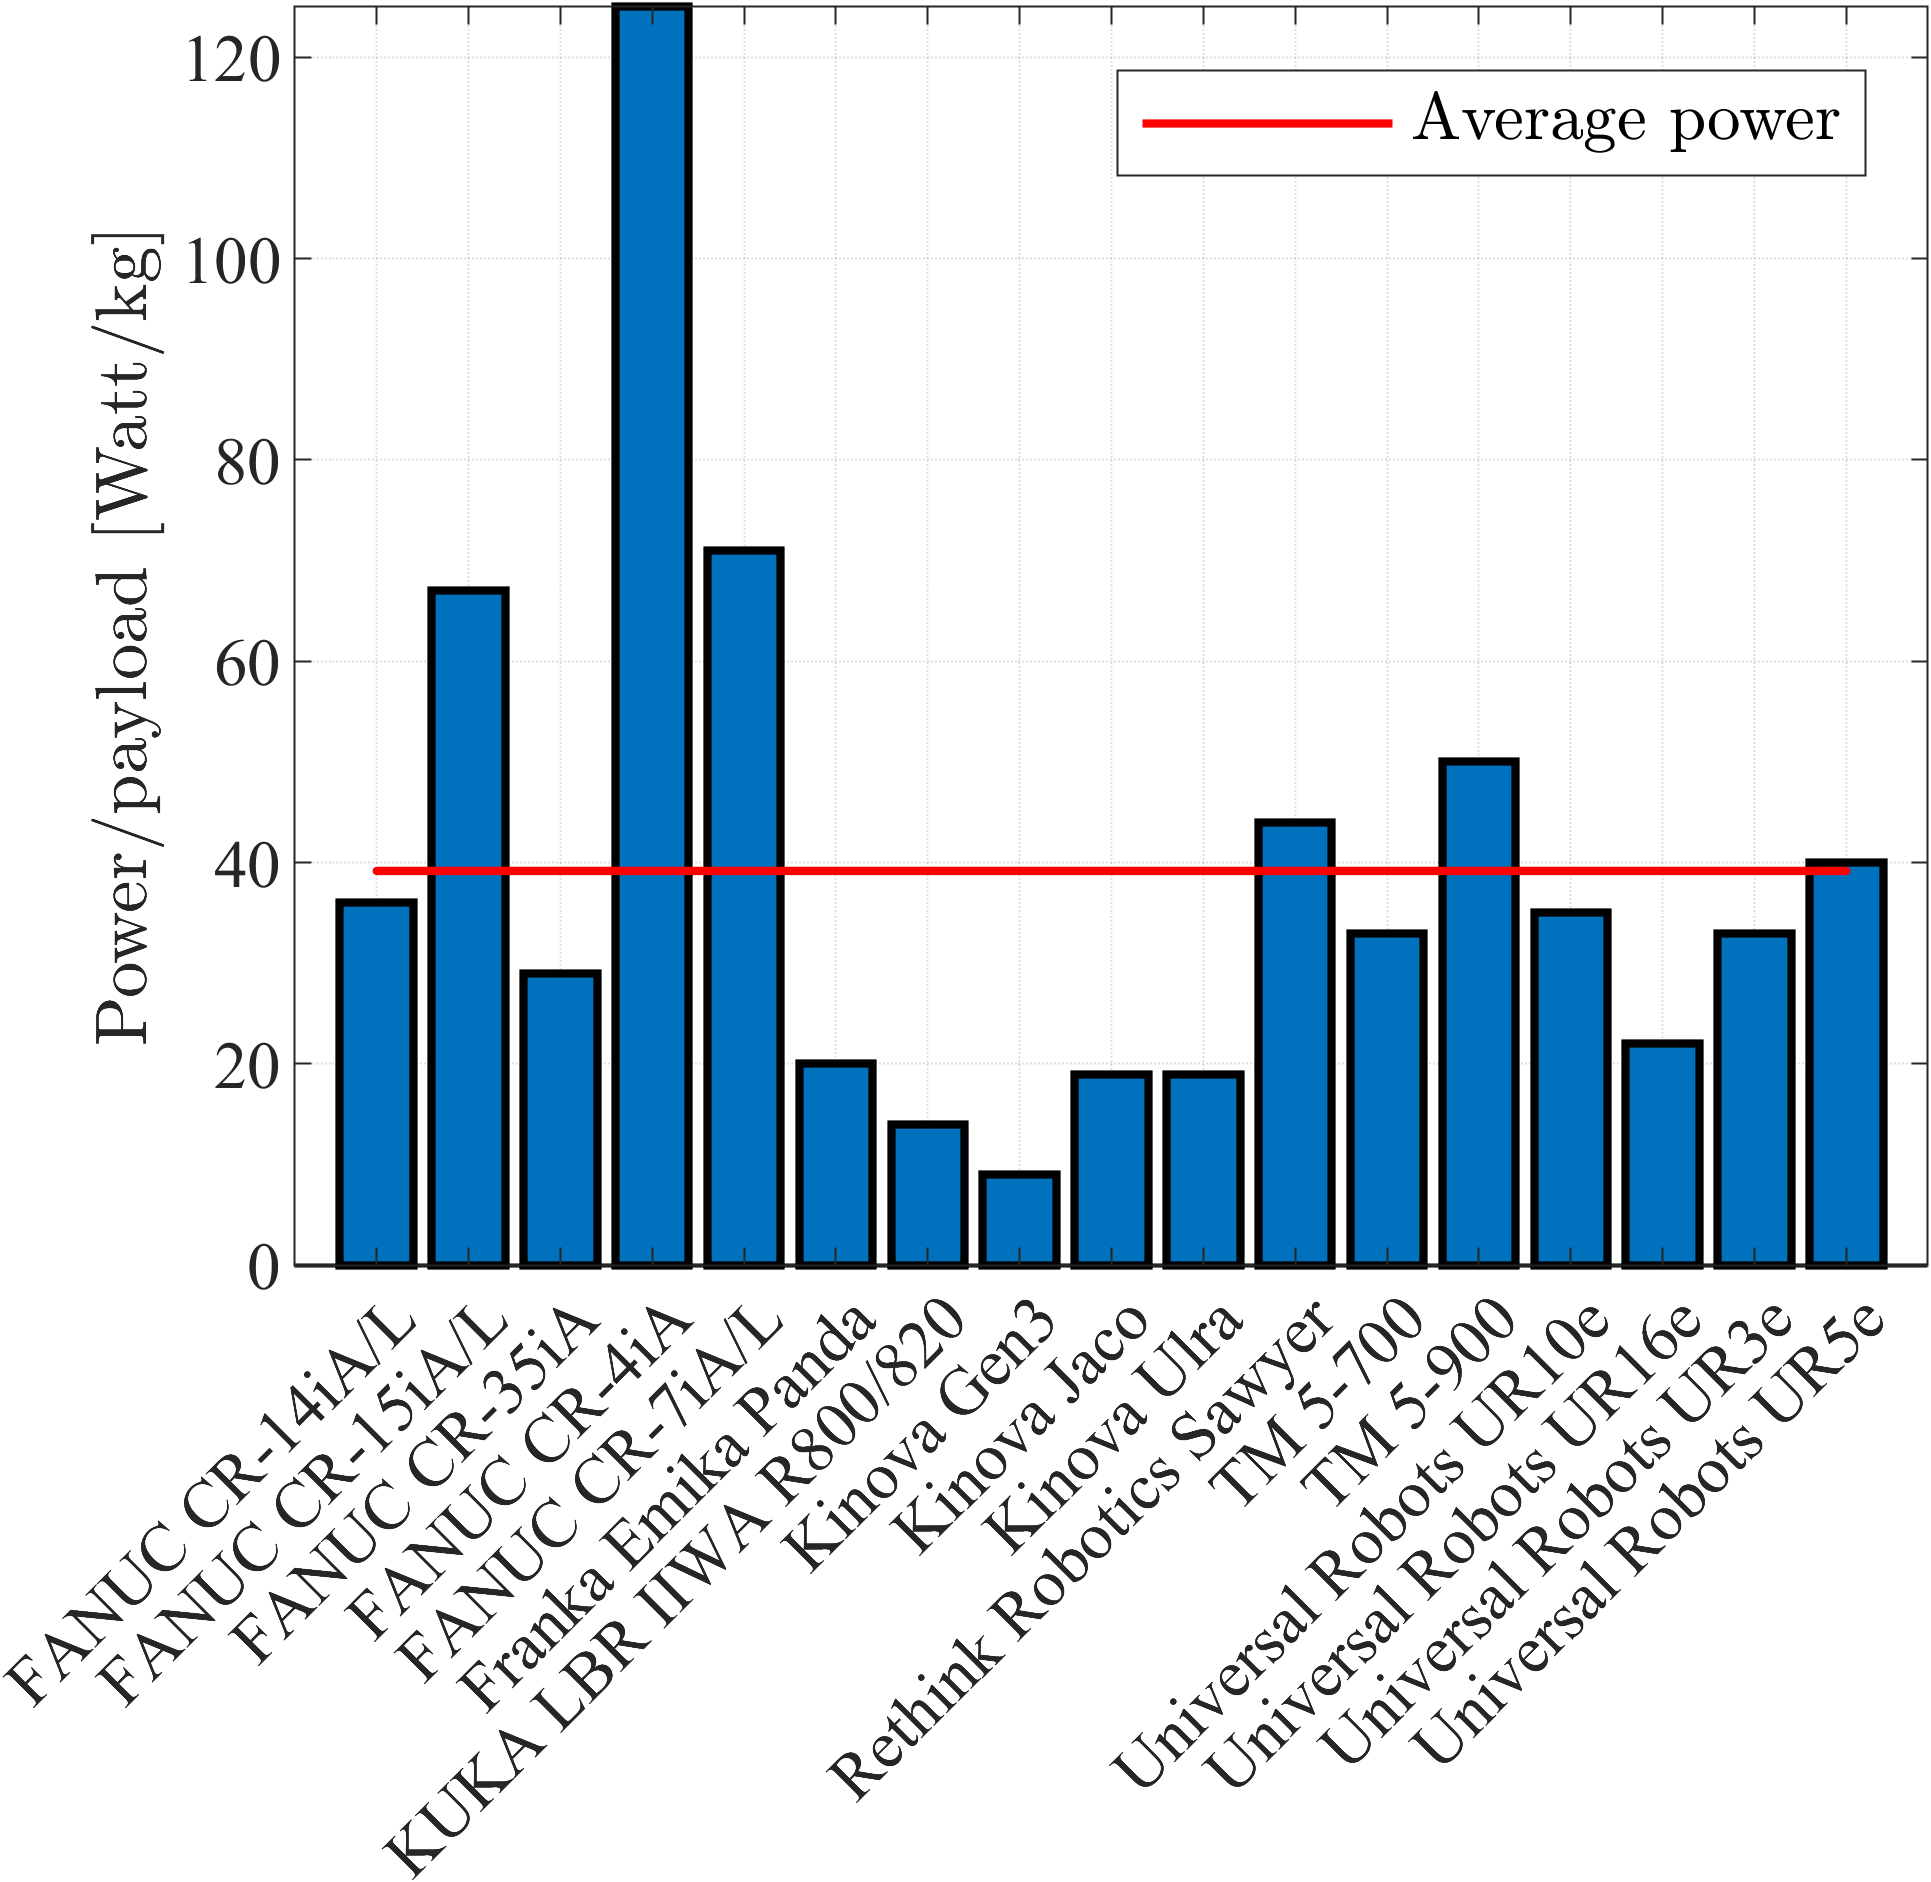
\includegraphics[width=0.45\textwidth]{cobot_watt_per_kg.png}
	\caption{Power consumption per payload for different cobots.}
	\label{fig:cobot_watt_per_kg}
\end{figure}
%---
To approximate the energy consumption of cobots we looked at the power consumption per payload of various manufacturers, see Fig.~\ref{fig:cobot_watt_per_kg} resulting in an average power consumption of approximately 40 W. Together with a typical power consumption of the robot controller of 60 W \cite{Heredia2023BreakingEnergyConsumption}, we consider a total of 100 W power demand. Similar to the industrial robots, the worldwide energy consumption was calculated assuming a 24/7 operation.





\renewcommand\refname{References and Notes}
\bibliography{bib/References.bib}
\bibliographystyle{Science}

\end{document}